\documentclass[11pt]{article}
\usepackage{graphicx,epic,html,makeidx}
\renewcommand{\hyperrefref}[4]{{\em #2}{$^{\mbox{\scriptsize\em \pageref{#4}}}$}}
%%% displayed synchronous programs
\makeatletter
\def\BEP{\begin{trivlist}\item[]
  \if@minipage\else\vskip\parskip\fi
  \leftskip\@totalleftmargin \advance\leftskip by 1\parindent
  \rightskip\z@ \parindent\z@ \parfillskip\@flushglue \parskip\z@
  \@tempswafalse \def\par{\if@tempswa\hbox{}\fi\@tempswatrue\@@par}
  \obeylines \tt \small \catcode``=13 \@noligs\frenchspacing\@vobeyspaces}
\def\EEP{\end{trivlist}}
\makeatother

\def\pp#1{\texttt{\small{#1}}}
\newcommand{\PP}[1]{\noindent{\textit{\textbf{#1}}}}

\def\X#1{$x_{#1}$}
\def\B#1{\texttt{#1}}

\def\se{\textit{syn{\small ERJY}}}
\def\sec{\textit{syn{\small ERJYcharts}}}
\def\sef{\textit{syn{\scriptsize ERJY}}}
\def\argos{\textsc{Argos}}
\def\lustre{\textsc{Lustre}}
\def\signal{\textsc{Signal}}
\def\esterel{\textsc{Esterel}}
\def\statecharts{\textsc{Statecharts}}
\def\synccharts{\textsc{SyncCharts}}
\def\java{\textsc{Java}$^{\mbox{\tiny TM}}$}
\def\matlab{\textsc{MATLAB}$^{\mbox{\tiny TM}}$}

\newcommand{\GO}[0]{{\small GO}}
\newcommand{\GOs}[0]{{\small GO}s}
\newcommand{\spc}[0]{\vspace{0.2cm}}

\newcommand{\vs}[0]{\vspace{1pt}}
\newcommand{\NTI}[1]{\textit{#1}}
\newcommand{\NTD}[1]{{\em #1}\label{#1}}
\newcommand{\NT}[1]{\index{#1@{\em #1}}\hyperref{#1}{#1}{}{#1}}
\newcommand{\NTZ}[2]{\index{#1@{\em #1}}\hyperref{#1}{#1#2}{}{#1}}
\newcommand{\KWI}[1]{{\index{#1@{\tt #1}}\tt #1}}
\newcommand{\T}[1]{{\tt #1}}
\newcommand{\is}[0]{$\Rightarrow$\vs}
\newcommand{\mto}[0]{$\mapsto$}
\newcommand{\Bopt}[0]{{\bf (}}
\newcommand{\optE}[0]{{\bf )\opt}}
\newcommand{\opt}[0]{$_{\textit{\scriptsize opt~}}$}
\newcommand{\Balt}[0]{{\bf (}}
\newcommand{\alt}[0]{\,$|$}
\newcommand{\altE}[0]{{\bf )$_\mbox{\em alt~}$}}
\renewcommand{\altE}[0]{{\bf )~}}
\newcommand{\lst}[0]{{...~~}}
\newcommand{\lsep}[1]{...\fbox{\scriptsize #1}...~~}
\newcommand{\rr}[0]{\vs\makebox[7mm]{}}

\newtheorem{example}{\bf Example}[section]
\newenvironment{BNF}{}{}

\def\codeinput#1{\IfFileExists{../tex_input/se.#1}{\input ../tex_input/se.#1}{\begin{center}chpt\_\thechapter\_#1.se\end{center}} {\footnotesize(cf. \texttt{chpt\_\thechapter\_#1.se})}}

\def\codefragment#1{\IfFileExists{../tex_input/se.#1}{\input ../tex_input/se.#1}{\begin{center}chpt\_\thechapter\_#1.se\end{center}}}

\def\codeinputref#1{\IfFileExists{../tex_input/se.#1}{\input ../tex_input/se.#1}{\begin{center}ref\_#1.se\end{center}} {\footnotesize(cf. \texttt{ref\_#1.se})}}

\def\codeinputuser#1{\IfFileExists{../tex_input/se.#1}{\input ../tex_input/se.#1}{\begin{center}user\_#1.se\end{center}} {\footnotesize(cf. \texttt{user\_#1.se})}}

\def\A{\mbox{${\cal A}$}}
\def\C{\mbox{${\cal C}$}}
\def\D{\mbox{${\cal D}$}}
\def\E{\mbox{${\cal E}$}}
\def\F{\mbox{${\cal F}$}}
\def\H{\mbox{${\cal H}$}}
\def\I{\mbox{${\cal I}$}}
\def\L{\mbox{${\cal L}$}}
\def\M{\mbox{${\cal M}$}}
\def\P{\mbox{${\cal P}$}}
\def\Q{\mbox{${\cal Q}$}}
\def\R{\mbox{${\cal R}$}}
\def\S{\mbox{${\cal S}$}}
\def\V{\mbox{${\cal V}$}}

\def\ARROW#1#2{\mbox{\def\arraystretch{0.1}\begin{tabular}{c}
$\ \scriptstyle #1\ $\\
\rightarrowfill\\
$\ \scriptstyle #2\ $\end{tabular}}}

\def\mkTitle#1{
\title{
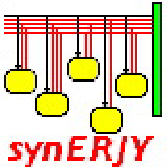
\includegraphics[height=50pt]{../pdf/se-logo}\hspace{0.5cm}
{\Huge \textit{\textbf{synERJY} 5.3}} \\ \vspace{1cm}\
       \textbf{#1}}

\author{\textit{Reinhard Budde}\\
\textit{Axel Poign\'e}\\
\textit{Karl-Heinz Sylla}\\
\ \\
\textbf{Fraunhofer Institut}\\\ \\ 
\textbf{Autonome intelligente Systeme}\\\ \\
\textbf{Fraunhofer AiS}\\\ \\\ \\
\\\ \\\ 
\\\  \\\ \\\ \\\ \\\ \\\textbf{\Large }
}

\date{\today}
}


\makeindex

\mkTitle{Language Reference Manual}

\begin{document}

\maketitle


\section*{Preface}

\se\footnote{\sef\ may be read as \textbf{syn}chronous
\textbf{e}mbedded \textbf{r}eactive \textbf{J}ava with a \textbf{y}
for the sound.} is a programming language and a design environment for
embedded reactive systems that combines two paradigms:
\begin{itemize}
    \item \emph{Object-oriented modelling} for a robust and flexible
    design.
      
    \item \emph{Synchronous execution} for precise modelling of
    reactive behaviour.
\end{itemize}
Highlights are that
\begin{itemize}
\item \se\ provides a deep embedding of the reactive behaviour into
      the object-oriented data model.
\item \se\ offers fine-grained integration of synchronous formalisms
      such as \esterel~\cite{esterel}, \lustre~\cite{lustre}, and
      \statecharts~\cite{statecharts}.\footnote{We recommend Halbwachs' book
      \emph{Synchronous Programming of Reactive Systems}~\cite{halbwachs} as 	an excellent introduction.}
\end{itemize}

The programming environment supports compilation, configuration,
simulation, and testing, as well as verification by model checking. 
Behavioural descriptions may be edited in graphical or in textual
form.  Code generators for efficient and compact code in C and several
hardware formats are available.

The \se\ language and its programming environment are developed
at the Fraunhofer Institut Autonome Intelligente Systeme.\footnote{The
development of \sef\ has been partially supported by the ESPRIT LTR
SYRF, ``Synchronous formalisms'', and the ESPRIT IIM Project CRISYS,
``Critical Systems and Instrumentation''.}  The programming
environment is freely available with a public domain license.
\newline

\noindent Contact:  
{\tt\small \{reinhard.budde,poigne,sylla\}@ais.fraunhofer.de}.



\newpage

\tableofcontents

\newpage

\section{Introduction}\label{Intro}

\se\ is a strongly typed object-oriented synchronous language for the
design of dependable embedded real-time software.  It is based on and
designed for maximal compatibility with \java.  The application area
of embedded systems demands for some restrictions, though:
\begin{itemize}
    \item Neither dynamic loading of packages

    \item nor threads are not supported, 
    
    \item arrays are two-dimensional at most, and
    
    \item primitive types are machine dependent.
\end{itemize}
The restrictions should be acceptable in that dynamic loading may
impair the predictability of behaviour, in particular with regard to
timing constraints. Arrays are one- or two-dimensional for supporting
a better memory layout. Two-dimensional arrays are ``square'' in that
the length of all rows and columns are equal.

On the other hand, the language has been
extended to accommodate synchronous programming of reactive behaviour. 
Particularly, \se\ features
\begin{itemize}
    \item signal based broadcast communication combined with

    \item parallel execution of and within objects,

    \item a compile-time schedule of activities (such as, e.g., method
    calls), and
    
    \item support for controller design and digital signal processing
    (by combining the imperative, state machine, and data-flow style of
     synchronous programming).
     
     \item support for vectors and matrices (i.e. arrays of fixed size)
     for signal processing.
         
    \item generation of efficient target code (ANSI-C and
    hardware formats).
\end{itemize}

The main concepts of the language are discussed at length in the 
complimentary {\em Introduction to \se}~\cite{language-introduction} 
that is recommended as a first reading. 


\subsection{The Reactive Execution Model}\label{reactive-execution}    

\paragraph{The synchrony hypothesis.}
Synchronous programming is a way of specifying discrete-time
(control) systems.  Many formalisms do the same. However, synchrony
as a paradigm avoids ad-hoc solutions and offers a mathematically
precise and, as we do believe, also a simple programming model. 

Synchronous behaviour is modelled as a machine that, on actuation,
reads the input sensors and is then \emph{decoupled from the
environment} to compute the subsequent \textit{state}\index{state} and
the value of the output signals, dispatches the output signals to the
environment, and waits for the next actuation.  Such an execution step
is called an \emph{instant}\index{instant}.

Execution, of course, takes time.  The delay does not cause harm as
long as it is sufficiently small in that an instant always terminates
before the next actuation takes place.  Then we may use the hypothesis
that input is sampled and output is generated ''at the same time''. 
The reaction appears to be ``instantaneous'' with regard to the
observable time scale in terms of activations.  Berry~\cite{esterel}
speaks of the \emph{synchrony hypothesis}\index{synchrony hypothesis}. 
Since time cannot be measured ``in between'' activations one sometimes
speaks of a ``zero time model''.

Sensors and signals are broadcast\index{broadcast} in synchronous
programming, i.e. at every instant there is a system-wide consistent
view of all sensors and signals.  In particular
\begin{itemize}
   \item the value of a signal is never updated at an instant after
   the value has been read once (\emph{write-before-read}
   strategy)\index{write-before-read}.
\end{itemize}
The subsequent state and the output signals must be uniquely
determined by the input sensors and the present state.

Synchronous languages nevertheless support concurrency.  Possible
non-determinism is resolved by the compiler.  If no deterministic
scheduling can be found, either due to a \emph{time race}\index{time
race} or due to a \emph{causality cycle}\index{causality cycle}, an
error message is issued and the program is rejected.

\paragraph{Synchronous formalisms.} Roughly, synchronous formalisms
may be distinguished according to whether they are based on control
flow or data flow.

The formalisms based on control flow (like
Esterel~\cite{esterel}\index{Esterel} or
Statecharts~\cite{statecharts})\index{Statemate} share the idea that
signals contribute to the control flow.  At an instant, a signal may
be emitted to be \emph{present}\index{signal!present}\index{present}. 
Otherwise it is \emph{absent}\index{signal!absent}\index{absent}.  One
may check for the presence of a signal.

Consider, for example, the following two simple automatons that are
supposed to run in parallel
\begin{center}
 {\tt\scriptsize
   \thinlines
   \setlength{\unitlength}{1pt}
   \begin{picture}(290,60)
   \put(0,0){
      \begin{picture}(130,60)
         \put(55,28){\normalsize $A_1$}
         \put(10,30){\circle{20}}
         \put(5,28){$st_1$}         
         \put(17,52){when (?a) \{ emit b;\}}
         \put(17,37){\bezier{200}(0,0)(41,20)(82,0)}
         \put(35,2){when (?a) \{ \}}
         \put(17,23){\bezier{200}(0,0)(41,-20)(82,0)}
         \put(95,39){\vector(2,-1){5}}
         \put(21,21){\vector(-2,1){4}}
         \put(107,30){\circle{20}}
         \put(102,28){$st_2$}    
      \end{picture}
   }
   \put(160,0){
      \begin{picture}(130,60)
         \put(55,28){\normalsize $A_2$}
         \put(10,30){\circle{20}}
         \put(5,28){$st_1'$}         
         \put(17,52){when (?b) \{ emit c;\}}
         \put(17,37){\bezier{200}(0,0)(41,20)(82,0)}
         \put(17,2){when (?b) \{ emit d;\}}
         \put(17,23){\bezier{200}(0,0)(41,-20)(82,0)}
         \put(95,39){\vector(2,-1){5}}
         \put(21,21){\vector(-2,1){4}}
         \put(107,30){\circle{20}}
         \put(102,28){$st_2'$}    
      \end{picture}
   }
   \end{picture}
 }
\end{center}
The expression \pp{?a} asks whether the signal \pp{a} is present. 
Hence, if the automatons are in state $st_1$ and state $st_1'$ and if
the signal \pp{a} is present the automaton $A_1$ moves from state
$st_1$ to state $st_2$ emitting \pp{b}.  In parallel the automaton
$A_2$ checks for the presence of \pp{b} provided it is in state
$st_1'$.  Since \pp{b} is present the $A_2$ moves from state $st_1'$
to state $st_2'$ emitting \pp{c}.  In that the signal \pp{b} is part
of the control flow.

Synchronous languages based on data flow (such as \lustre\cite{lustre}
\index{Lustre} and \signal\cite{signal})\index{Signal} are inspired by 
difference equations\index{difference equation} such as
s
%
{\small
\begin{eqnarray*}
z(n) & = & 0.5*z(n-1) + 0.3*y(n) + 0.2*x1(n)\\
y(n) & = & 0.5*x1(n) + 0.5 * x2(n)
\end{eqnarray*}
}
%
Each of the equations is evaluated at time $n$ to compute a new value
of the respective variable.  $x1$ and $x2$ are assumed to be inputs.

For difference equations, the order of evaluation is determined by the
variables only: at an instant, the value of a variable must be
computed before it is used in some equation.

It is a minor shift to rewrite the difference equations as \emph{data
flow equations}\index{data flow}.  Consider each of the variables as
to refer to an indexed sequence of data, a \emph{data flow}, and we
assume that operations like addition and multiplication are defined
point-wise.
%
{
\small
\begin{eqnarray*}
y & = & 0.5*x1 + 0.5 * x2\\
z & = & 0.5*pre(z) + 0.3*y + 0.2*x1
\end{eqnarray*}
}
%
For the second equation, we need what is called a \emph{time shift
operator} \pp{pre} such that $\pp{pre}(z)(n) = z(n-1)$.

\subsection{Programming in \se}

\se smoothly integrates the control flow and data flow flavours of
synchronous programming with object-oriented structuring principles. 
We superficially discuss two, somewhat artificial, examples to
illustrate the integration.\footnote{At this stage, one should not
expect fully to grasp the meaning of the programs.  We recommend
\cite{language-introduction} as a first reading for a deeper
understanding of the language.}

\paragraph{Synchrony and object-orientation.}

The basic structure of \se\ compares to that of \java. An application is 
specified in terms of classes.  A class with a method \texttt{main} is 
a \emph{configuration class}\index{configuration class} from which an 
application may be generated.

Classes in \se\ may be reactive, i.e. exhibit some reactive 
behaviour. Here is a simple example.
%
\codeinputref{basic}
%
There is sensor \texttt{button}, and 
there is a signal \texttt{red\_led} that may be emitted. The reactive 
code is embedded using the \texttt{active} statement. It just says 
that the program waits for the presence of the sensor 
\texttt{button} (The notation \texttt{?button} states that one asks 
for the presence of a sensor or signal), and then immediately emits
the signal \texttt{red\_led}. Then it pauses till the next instant 
to wait again for the presence of the sensor \texttt{button}.

Sensor and signal types\index{signal type}\index{type!signal} behave
like reference types.  They are created using a constructor.  Here the
constructors have objects of type
\texttt{SimInput}\index{SimInput@\texttt{SimInput}} and
\texttt{SimOutput}\index{SimOutput@\texttt{SimOutput}} as arguments. 
These specify the interaction with the simulator of the \se\ tool set. 
In general, ``input'' and ``output'' objects as parameters of a sensor
and signal constructor specify the interface of a sensor or signal to
the environment.  Sensors have parameters of type ``input'', signals
have parameters of type ``output''.

If several reactive objects are generated in an application, the 
objects executes in parallel but, since they may share sensors and
signals, some scheduling restrictions are imposed.

The method \texttt{main} is an infinite loop that calls the system
method \texttt{instant}\index{instant@\texttt{instant}}.  This method
executes one step of the reactive machine.  It returns an exception
code as value.  The value $0$ states that no exception is thrown.

\paragraph{Integration of synchronous formalism.}
We demonstrate the integration of two styles -- the automatons style and 
the data flow style -- again by a simple example.
%
\codeinputref{up-and-down-counter-ref}
%
If started the signal \texttt{count} is emitted with value $0$, and
then the automaton immediately enters state \texttt{up}.  During being
in state \texttt{up} the data flow equation \texttt{count :=
pre(count) + 1;} is evaluated.  The flow term on the right hand side
states that its value at an instant is computed by increasing the
value of the signal \texttt{count} at the previous instant by $1$. 
When the counter has value $10$ state changes from \texttt{up} to
\texttt{down} (the notation \texttt{\$count} states that the value of
a signal is accessed).  During being in state \texttt{down} the other
flow equation is evaluated decreasing the counter.

Note that signals can be emitted as well as constrained by a flow
equation.  This unification of signals as known of \esterel\ and flow
variables as known of \lustre\ is one of the particular highlights of
\se.  In general, we say that a signal is \emph{updated} either when
it is emitted or constrained by a flow equation.

\subsection{Presentation}

This reference manual focuses on the synchronous extensions, though it
aims for completeness.  The style of presentation follows that of the
\java\ language specification in \cite{java}.  which we strongly
recommend as complimentary reading.  We stress the differences between
\se\ and \java.

\subsection{Compilation and Programming Environment}

\se\ is compiled to a simple sub-language of ANSI-C as intermediate
code for cross-compiling to different target architectures.  The
generated code is fairly efficient in that it may run even on small
micro controllers.  Restricted compilation schemes additionally
generate several hardware formats for pure control applications.

\se\ provides a programming environment including a graphic editor for
state machine and a simulator for tracing the values of sensors, 
signals, and fields.
These are documented in complimentary user manual~\cite{user-manual}.

\newpage
\section{Grammars}

We assume the reader to be familiar with context-free
grammars\index{grammar!context-free} which are crucial for syntactic
representation.\footnote{A short overview may be found in
\cite{java}.} The notation for context-free grammars follows that of
the \java\ reference manual.  Terminal
symbols\index{symbol!terminal}\index{terminal} are shown in
\texttt{fixed width} font, nonterminals\index{symbol!non-
terminal}\index{non-terminal} in \textit{italic}.  A syntactic
definition\index{rule!context-free}\index{context-free} is of the form
\begin{quote}
   {\it Arguments}\textit{:}\\*
    \rr\ {\it Argument}\\*
    \rr\ {\it Argument}\ \ {\it Arguments}
\end{quote}
The nonterminal being defined is in the first line followed by a
colon, the alternatives listed in the following lines.  Long
definitions may be extended to a second line using indentation. 
Optional constructs are indicated by the subscript ~\ldots~\opt.

In the HTML-version of this document, a nonterminal is linked to its
definition.  In the \TeX-version, superscripts of nonterminals specify
the page number of its definition.

The lexical grammar has the non-terminal \NT{Input} as start symbol. 
It specifies the translation of streams of ASCII input characters into
input token.

The syntactic grammar specifies the sequences of input tokens that
form a syntactically correct program.  Its starting symbol is
\NT{CompilationUnit}.

\newpage
\section{Lexical structure}

\subsection{Lexical Translations}
The lexical translation transforms a sequence of ASCII characters into
a sequence of tokens that are the terminal symbols of the syntactic
grammar (\se\ does not support Unicode). 

\subsection{Line Terminators}
Lines are terminated by the ASCII characters CR, or LF, or CR LF. The
latter is counted as one line terminator.
\begin{quote}
    \NTD{LineTerminator}\textit{:}\\*
     \rr\ the ASCII LF character, also known as "newline"\\*
     \rr\ the ASCII CR character, also known as "return"\\*
     \rr\ the ASCII CR character followed by the ASCII LF character\\*
    \NTD{InputCharacter}\textit{:}\\*
     \rr\ ASCII Characters but not CR or LF
\end{quote}

\subsection{Input Elements and Tokens}
Input elements that are not whitespace or comments are tokens.  Tokens
are the terminals of the syntactic grammar.
\begin{quote}
    \NTD{Input}\textit{:}\\*
    \rr\ \NT{InputElements}\opt\\*
    \NTD{InputElements}\textit{:}\\*
    \rr\ \NT{InputElement}\\*
    \rr\ \NT{InputElements} \NT{InputElement}\\*
    \NTD{InputElement}\textit{:}\\*
    \rr\ \NT{WhiteSpace}\\*
    \rr\ \NT{Comment}\\*    
    \rr\ \NT{Token}\\*
    \NTD{Token}\textit{:}\\*
    \rr\ \NT{Identifier}\\*
    \rr\ \NT{Keyword}\\*
    \rr\ \NT{Literal}\\*
    \rr\ \NT{Separator}\\*
    \rr\ \NT{Operator}\\*
%     \NTD{Sub}\textit{:}\\*
%     \rr\ the ASCII SUB character, also known as "control-Z"
\end{quote}

\subsection{Whitespace}
White space is defined as the ASCII space, horizontal tab, and form
feed characters, as well as line terminators
\begin{quote}
    \NTD{WhiteSpace}\textit{:}\\*
    \rr\ the ASCII SP character, also known as "space"\\*
    \rr\ the ASCII HT character, also known as "horizontal tab"\\*
    \rr\ the ASCII FF character, also known as "form feed"\\*
    \rr\ \NT{LineTerminator}
\end{quote}

\subsection{Comment}\index{comment}
There are two kinds of comments: an in-line comment of the form
``$\texttt{/*}\ \ \textit{comment}\ \ \texttt{*/}$'', and an end of
line comment of the form ``$\texttt{//}\ \ \textit{comment}$''.  The
grammar rules are:
\begin{quote}
    \NTD{Comment}\textit{:}\\*
    \rr\ \NT{TraditionalComment}\\*
    \rr\ \NT{EndOfLineComment}\\*
% 
    \NTD{TraditionalComment}\textit{:}\\*
    \rr\ \T{/}\ \T{*}\ \NT{NotStar}\ \NT{CommentTail}\\*
% 
    \NTD{EndOfLineComment}\textit{:}\\*
    \rr\ \T{/}\T{/}\ \NT{CharactersInLine}\opt\ 
\NT{LineTerminator}\\*
% 
    \NTD{CommentTail}\textit{:}\\*
    \rr\ \T{*}\ \NT{CommentTailStar}\\*
    \rr\ \NT{NotStar}\ \NT{CommentTail}\\*
% 
    \NTD{CommentTailStar}\textit{:}\\*
    \rr\ \T{/}\\*
    \rr\ \T{*}\ \NT{CommentTailStar}\\*
    \rr\ \NT{NotStarNotSlash}\ \NT{CommentTail}\\*
% 
    \NTD{NotStar}\textit{:}\\*
    \rr\ \NT{InputCharacter} but not \texttt{*}\\*
    \rr\ \NT{LineTerminator}\\*
% 
    \NTD{NotStarNotSlash}\textit{:}\\*
    \rr\ \NT{InputCharacter} but not \texttt{*} or \texttt{/}\\*
    \rr\ \NT{LineTerminator}\\*
% 
    \NTD{CharactersInLine}\textit{:}\\*
    \rr\ \NT{InputCharacter}\\*
    \rr\ \NT{CharactersInLine}\ \NT{InputCharacter}
\end{quote}

\subsection{Identifiers}\index{identifier}
An identifier is an unlimited-length sequence of ASCII letters and
ASCII digits, the first of which must be a letter or \T{\_}.  An 
identifier cannot be a keyword, a boolean literal, or the null literal. It is 
not allowed to contain two consecutive \T{\_}.
\begin{quote}
    \NTD{Identifier}\textit{:}\\*
    \rr\ \NT{IdentifierChars}\\*
    \rr\  \ \mbox{but not a \NT{Keyword} or \NT{BooleanLiteral} or 
    \NT{NullLiteral}}\\*
    \NTD{IdentifierChars}\textit{:}\\*
    \rr\ \NT{ASCIILetter}\\*
    \rr\ \NT{IdentifierChars} \NT{ASCIILetterOrDigit}\\*
    \NTD{ASCIILetter}\textit{:}\\*
    \rr\ {\it any ASCII character}\\*
    \NTD{ASCIILetterOrDigit}\textit{:}\\*
    \rr\ {\it any ASCII character that is a ASCII letter-or-digit}
\end{quote}
Two identifiers are equal if they consist of the same sequence of
ASCII letters.

\subsection{Labels}\label{labels}
Labels are used to mark a position within a program.  Labels\index{label}
are identifiers followed by two colons (no blanks in between).

\begin{quote}
    \NTD{Label}\textit{:}\\*
    \rr\ \NT{Identifier}\KWI{::}
\end{quote}

\subsection{Keywords}\index{keyword} The following words are reserved as 
keywords:

\begin{quote}
   \NTD{Keyword}\textit{:}\\*
   \rr \NT{UsedKeyword}\\*
   \rr \NT{ReservedKeyword}\\* 
\NTD{UsedKeyword}\textit{: one of}\\*
{\small
\begin{tabular}{lllll}

    \quad 
    \texttt{abstract}&
    \texttt{do}&
    \texttt{implements}&
    \texttt{parameter}&
    \texttt{sustain}\\

    \quad 
    \texttt{activate}&
    \texttt{dt}&
    \texttt{import}& 
    \texttt{post}&
    \texttt{switch}\\

    \quad 
    \texttt{active}&
    \texttt{during}&
    \texttt{import\_from\_C}& 
    \texttt{pre}&
    \texttt{then}\\

    \quad 
    \texttt{assert}&
    \texttt{else}&
    \texttt{init }& 
    \texttt{precedence}&
    \texttt{this}\\

    \quad 
    \texttt{automaton}&
    \texttt{emit}&
    \texttt{instanceof}& 
    \texttt{private}&
    \texttt{throw}\\

    \quad 
    \texttt{await}&
    \texttt{entry}&
    \texttt{instant}& 
    \texttt{ptl}&
    \texttt{transient}\\

    \quad 
    \texttt{blacboard}&
    \texttt{exit}&
    \texttt{interface}& 
    \texttt{protected}&
    \texttt{until}\\

    \quad 
    \texttt{break}&
    \texttt{export\_to\_C}&
    \texttt{interrupt}&
    \texttt{public}&
    \texttt{void}\\

    \quad 
    \texttt{cancel}&
    \texttt{extends}&
    \texttt{invariant}& 
    \texttt{reactive}&
    \texttt{volatile}\\

    \quad 
    \texttt{case}&
    \texttt{fairness}&
    \texttt{loop}& 
    \texttt{return}&
    \texttt{when}\\

    \quad 
    \texttt{class}&
    \texttt{final}&
    \texttt{ltl}& 
    \texttt{schedule}&
    \texttt{while}\\

    \quad 
    \texttt{const}&
    \texttt{for}&
    \texttt{native}& 
    \texttt{state}&
    \texttt{}\\

    \quad
    \texttt{continue}&
    \texttt{formula}&
    \texttt{new}&
    \texttt{static}&
    \texttt{}\\

    \quad 
    \texttt{ctl}&
    \texttt{goto}&
    \texttt{next}& 
    \texttt{strictfp}&
    \texttt{}\\

    \quad 
    \texttt{current}&
    \texttt{halt}&
    \texttt{node}& 
    \texttt{strongly}&
    \texttt{}\\
    
    \quad 
    \texttt{default}&
    \texttt{if}&
    \texttt{nothing}& 
    \texttt{super}&
    \texttt{}\\
\end{tabular}    
} 
   
{\small
    \NTD{ReservedKeyword}\textit{: one of}\\*
     \begin{tabular}{lllll}
    
    \quad 
    \texttt{catch}&
    \texttt{finally}&
    \texttt{simple}&
    \texttt{}&
    \texttt{}\\

    \quad 
    \texttt{equal}&
    \texttt{not\_equal}&
    \texttt{synchronized}& 
    \texttt{}&
    \texttt{}\\
\end{tabular}    
}    
\end{quote}

\subsection{Literals}

A \emph{literal}\index{literal} present a value of primitive type, of 
\texttt{String} type, or of \texttt{null} type.

\begin{quote}
    \NTD{Literal}\textit{:}\\*
    \rr\ \NT{IntegerLiteral}\\*
    \rr\ \NT{FloatingPointLiteral}\\*
    \rr\ \NT{BooleanLiteral}\\*
    \rr\ \NT{CharacterLiteral}\\*
    \rr\ \NT{StringLiteral}\\*
    \rr\ \NT{NullLiteral}\\*
    \rr\ \NT{TimeLiteral}
\end{quote}

\paragraph{Integer literals.}\index{literal!integer} 

An integer literal may be a decimal literal (base 10) or a 
hexadecimal literal (base 16). Octal literals are not supported.
\begin{quote}
    \NTD{IntegerLiteral}\textit{:}\\*
    \rr\ \NT{DecimalNumeral}\\*
    \rr\ \NT{HexNumeral}\\*
%     
    \NTD{DecimalNumeral}\textit{:}\\*
    \rr\ \T{0}\\*
    \rr\ \NT{NonZeroDigit}\ \NT{Digits}\opt\\*
%     
    \NTD{Digits}\textit{:}\\*
    \rr\ \NT{Digit}\\*
    \rr\ \NT{Digits}\ \NT{Digit}\\*
%     
    \NTD{Digit}\textit{:}\\*
    \rr\ \T{0}\\*
    \rr\ \NT{NonZeroDigit}\\*
% 
    \NTD{NonZeroDigit}\textit{: one of}\\* 
    \rr\ \T{1}\ \T{2}\
    \T{3}\ \T{4}\ \T{5}\ \T{6}\ \T{7}\ \T{8}\ \T{9}\\*
% 
    \NTD{HexNumeral}\textit{:}\\*
    \rr\ \T{0 x}\ \NT{HexDigits}\\*
    \rr\ \T{0 X}\ \NT{HexDigits}\\*
% 
    \NTD{HexDigits}\textit{:}\\*
    \rr\ \NT{HexDigit}\\*
    \rr\ \NT{HexDigit}\ \NT{HexDigits}\\*
    
% 
    \NTD{HexDigit}\textit{: one of}\\* \rr\ \T{0}\ \T{1}\ \T{2}\
    \T{3}\ \T{4}\ \T{5}\ \T{6}\ \T{7}\ \T{8}\ \T{a}\ \T{b}\
    \T{c}\ \T{d}\ \T{e}\ \T{f}\ \T{A}\ \T{B}\ \T{C}\ \T{D}\
    \T{D}\ \T{F}
\end{quote}
An integer literal is of an integral type (cf. 
Section~\ref{primitivetypes}).  The type is determined automatically
by choosing the most appropriate type according to the context.  If
the context does the type the least possible type is chosen according
to the type hierarchy of integral types (cf. 
Section~\ref{primitivetypes}).  For instance, the literal \T{15} is
of type \KWI{byte} (and, hence of all the super types of \T{byte}). 
Applying a cast may change the type, e.g. \T{(int)15} is of type
\KWI{int}.

\paragraph{Floating-Point literals.}\index{literal!floating point}
The elements of the types \KWI{float} and \KWI{double} conform with the
IEEE 754 32-bit single-precision and 64-bit double-precision binary
floating-point formats.
\begin{quote}
    \NTD{FloatingPointLiteral}\textit{:}\\*
    \rr\ \NT{Digits}\ \T{.}\ \NT{Digits}\opt \NT{ExponentPart}\opt  
    \NT{FloatTypeSuffix}\\*
    \rr\ \T{.}\opt \NT{Digits}\ \NT{ExponentPart}\opt  
    \NT{FloatTypeSuffix}\\*
    \rr\ \NT{Digits}\ \NT{ExponentPart}\ \NT{FloatTypeSuffix}\\*
    \rr\ \NT{Digits}\ \NT{ExponentPart}\opt \NT{FloatTypeSuffix}\\*
% 
    \NTD{ExponentPart}\textit{:}\\*
    \rr\ \NT{ExponentIndicator}\ \NT{SignedInteger}\\*
% 
    \NTD{ExponentIndicator}\textit{: one of}\\*
    \rr\ \T{e}\ \T{E}\\*
% 
    \NTD{SignedInteger}\textit{:}\\*
    \rr\ \NT{Sign}\opt \NT{Digits}\\*
% 
    \NTD{Sign}\textit{: one of}\\*
    \rr\ \T{+}\quad \T{-}\\*
% 
     \NTD{FloatTypeSuffix}\textit{: one of}\\*
     \rr\ \T{f}\quad \T{F}\quad \T{d}\quad \T{D}\\*
\end{quote}
Floating point literals are of type \KWI{double} by default.

\paragraph{Boolean literals.}\index{literal!boolean}\index{true@\texttt{true}}
\index{false@\texttt{false}}
As usual, there are two Boolean values, true and false.
\begin{quote}
    \NTD{BooleanLiteral}\textit{: one of}\\*
    \rr\ \KWI{true}
    \rr\ \KWI{false}
\end{quote}

\paragraph{Character literals.}\index{literal!character}
In contrast to \java, character literal are pure ASCII.
\begin{quote}
    \NTD{CharacterLiteral}\textit{:}\\*
    \rr\ \T{'}\ \NT{SingleCharacter}\ \T{'}\\*
%      \rr\ \T{'}\ \NT{EscapeSequence}\ \T{'}\\*
% 
    \NTD{SingleCharacter}\textit{:}\\*
    \rr\ \NT{InputCharacter}\  \mbox{but not {\tt '} or {\tt \ }}
\end{quote}


\paragraph{String literals.}\index{literal!string}
A string literal consists of zero or more characters enclosed in 
double quotes. 
\begin{quote}

    \NTD{StringLiteral}\textit{:}\\*
     \rr\ \T{"}\ \NT{StringCharacters}\opt \T{"}\\*
% 
    \NTD{StringCharacters}\textit{:}\\*
    \rr\ \NT{StringCharacter}\\*
    \rr\ \NT{StringCharacters}\ \NT{StringCharacter}\\*
% 
    \NTD{StringCharacter}\textit{:}\\*
    \rr\ \NT{InputCharacter} \mbox{but not " or \texttt{\\}} \\*
%     \rr\ \NT{EscapeSequence}
\end{quote}

\paragraph{Null literal.}\index{literal!null@\texttt{null}}

There is only one value of null type, the null reference, which always
is of null type.

\begin{quote}
    \NTD{NullLiteral}\textit{:}\\*
    \rr\ \KWI{null}
\end{quote}

\paragraph{Time literals.}\index{literal!time}
A \emph{time literal} consists of a decimal numeral followed by one 
time suffixes \texttt{msec}, \texttt{usec}, \texttt{sec}, 
\texttt{min}, or \texttt{hour} with the obvious intended meaning. For 
notational convenience, a time literal may be of the format
\T{12.3456sec}.

\begin{quote}
    \NTD{TimeLiteral}\textit{:}\\*
    \rr\ \NT{DecimalNumeral}\ \NT{TimeUnitSuffix}\\*
    \rr\ \NT{DecimalNumeral}\ \T{.}\ \NT{DecimalNumeral}\ \KWI{sec}\\*
%     
    \NTD{TimeUnitSuffix}\textit{: one of}\\*
    \rr\ \KWI{msec}\ \KWI{usec}\ \KWI{sec}\ \KWI{min}\ \KWI{hour}    
\end{quote}


\subsection{Separators}\index{separators}

The following ASCII characters are the separators:

\begin{quote}
    \NTD{Separator}\textit{: one of}\\*
    \rr\ \T{(}\quad \T{)}\quad \T{\{}\quad \T{\}}\quad 
\T{[}\quad \T{]}
    \quad \T{<}\quad \T{>}\quad \T{;}\quad \T{,}\quad \T{.}\quad 
\T{:}
\end{quote}


\subsection{Operators}\index{operators}

The following ASCII characters are the separators:

\begin{quote}
    \NTD{Operator}\textit{: one of}\\*
{\tt
\rr\   \begin{tabular}{ccccccccccc}
       =  & \textless & \textgreater & ! & \textasciitilde & | & ? & 
: & & &  \\
       == & <= & >= & != & \&\& & || & ++ & -- & & &  \\
       + & - & * & / & \& & | & \textasciicircum & \% & << & >> & >>> 
\\
       += & -= & *= & /= & \&= & |= & \textasciicircum = & \%= & <<= &
       >>= & >>>= \\
   \end{tabular}
} 
\end{quote}


\newpage
\section{Types, Values, and Variables}

\subsection{Kinds of Types} 

Types are either \emph{primitive types}\index{type!primitive}\index{primitive 
type}, \emph{reference types}\index{type!reference}\index{reference type}, 
or signal types\index{type!signal}\index{signal type}. There is a special 
\emph{null type}\index{null type}\index{type!null}\index{null type}
with the only value being the null reference \texttt{null}.
\begin{quote}
    \NTD{Type}\textit{:}\\*
    \rr\ \NT{PrimitiveType}\\*
    \rr\ \NT{ReferenceType}\\*
    \rr\ \NT{SignalType}
\end{quote}

Every variable and every expression has a type that can be determined
at compile time.

\subsection{Primitive types}\label{primitivetypes}
\index{type!primitive}\index{primitive type}

Compared to \java, there are a couple of new primitive types.
\begin{itemize}
   \item the type \texttt{time}\index{time@\texttt{time}} (cf.  Section \ref{time})
   
   \item the integral types \texttt{uint8}\index{uint8@\texttt{uint8}}, 
         \texttt{uint16}\index{uint16@\texttt{uint16}},
         \texttt{uint32}\index{uint32@\texttt{uint32}}, and 
         \texttt{uint64}\index{uint64@\texttt{uint64}} which enhance the 
         efficiency of compilation, in particular with regard to micro 
         controllers.
\end{itemize}

\begin{quote}
    \NTD{PrimitiveType}\textit{:}\\*
    \rr\ \NT{NumericType}\\*
    \rr\ \KWI{boolean}\\*
    \rr\ \KWI{bool}\ \textit{as shorthand}\\*
    \rr\ \KWI{time}\\*
% 
    \NTD{NumericType}\textit{:}\\*
    \rr\ \NT{IntegralType}\\*
    \rr\ \NT{FloatingPointType}\\*
% 
    \NTD{IntegralType}\textit{: one of}\\*
    \rr\ \KWI{char}\\*
    \rr\ \KWI{byte}\ \ \ \KWI{unit8}\\*
    \rr\ \KWI{short}\ \ \KWI{uint16}\\*     
    \rr\ \KWI{int}\ \ \ \ \KWI{uint32}\\*         
    \rr\ \KWI{long}\ \ \ \KWI{uint64}\\*
% 
    \NTD{FloatingPointType}\textit{: one of}\\*
    \rr\ \KWI{float}\quad \KWI{double}
\end{quote}

The values of numerical type depend on the target machine that can 
range up to small target machines. Hence the value scopes specified 
below are ``typical'' for a variety of machines.

The value of a variable of primitive type can be changed only by
assignment.


\paragraph{Integral types and values.}\index{type!integral}\index{integral type}

The values of integral types have the following format and ranges:
\begin{itemize}
    \item  type \texttt{byte}\index{byte@\texttt{byte}}: signed 8 bit\\
    (\emph{synonym}: \texttt{int8})

    \item  type \texttt{char}\index{char@\texttt{char}}: unsigned 8 bit\\ 
    (\emph{synonyms}: 
    \texttt{uint8}, \texttt{unsigned int8}, \texttt{unsigned byte})

    \item  type \texttt{short}\index{short@\texttt{short}}: signed 16 bit\\ 
    (\emph{synonym}: \texttt{int16})

    \item  type \texttt{uint16}: unsigned 16 bit\\ (\emph{synonyms}: 
    \texttt{uint16}, \texttt{unsigned int16}, \texttt{unsigned int})

    \item  type \texttt{int}\index{int@\texttt{int}}: signed 32 bit\\ 
    (\emph{synonym}: \texttt{int32})

    \item type \texttt{uint32}: unsigned 32\\ (\emph{synonyms}:
    \texttt{uint32}, \texttt{unsigned int32}, \texttt{unsigned int})

    \item type \texttt{long}\index{long@\texttt{long}}: signed 64 bit\\ 
    (\emph{synonym}: \texttt{int64})

    \item type \texttt{uint64}: unsigned 64 bit\\ (\emph{synonyms}:
    \texttt{uint64}, \texttt{unsigned int64}, \texttt{unsigned long})
\end{itemize}
%
An integer literal is ``polymorphic'' in that it may be of any type
such that its value is a value of that type, e.g. \texttt{1} is of any
of the integral types, \texttt{-1} is of any of the signed types. 
Each literal has a most specific type that is the type that comprises
its value, and that is the smallest such type.  Most specific types
are, e.g.
\begin{itemize}
\item \texttt{1} is of type \texttt{char},
\item \texttt{-1} is of type \texttt{byte},
\item \texttt{256} is of type \texttt{uint16},
\item \texttt{-128} is of type \texttt{short}, etc.
\end{itemize}
The type of an integral literal will resolved by the context it is used in
(cf. Section \ref{conversion}). 


\noindent The operations related to integral types are:
\begin{itemize}
    \item relational operators \texttt{==} and \texttt{!=} 
(\emph{equal}
    and \emph{not equal}).

    \item comparison operators \texttt{<}, \texttt{<=}, \texttt{>},
    and \texttt{>=} (\emph{less than}, \emph{less than or equal},
    \emph{greater than}, and \emph{greater than or equal}).

    \item unary numerical operators \texttt{+} and \texttt{-}
    (\emph{plus} and \emph{minus})

    \item binary numerical operators \texttt{+}, \texttt{-},
    \texttt{*}, and \texttt{/} (\emph{plus}, \emph{minus},
    \emph{multiplication}, and \emph{division}).

    \item unary numerical operators \texttt{++} and \texttt{--}
    (\emph{increment} and \emph{decrement} both prefix and postfix)

    \item unary logical operator \texttt{$\sim$} (\emph{complement})
    
    \item binary logical operators \texttt{\&}, \texttt{|},
    \texttt{\&\&}, and \texttt{||} (\emph{and}, \emph{or},
    \emph{conditional and}, and \emph{conditional or})

    \item shift operators \texttt{<<}, \texttt{>>}, and \texttt{>>>}
    (\emph{left shift}, \emph{right shift}, and \emph{arithmetic right
    shift})

\end{itemize}

\paragraph{Floating-points type and values.}\index{type!floating
point}\index{floating point type}
The values of inegral types have the following format and ranges:
\begin{itemize}
    \item  type \texttt{float}\index{float@\texttt{float}}: 32 bit floating 
    point 
    
     \item  type \texttt{double}\index{double@\texttt{double}}: 64 bit 
     floating point
\end{itemize}
%
\noindent The operations related to floating-point types are:
\begin{itemize}
    \item relational operators \texttt{==} and \texttt{!=} 
(\emph{equal}
    and \emph{not equal}).

    \item comparison operators \texttt{<}, \texttt{<=}, \texttt{>},
    and \texttt{>=} (\emph{less than}, \emph{less than or equal},
    \emph{greater than}, and \emph{greater than or equal}).

    \item unary numerical operators \texttt{+} and \texttt{-}
    (\emph{plus} and \emph{minus})

    \item binary numerical operators \texttt{+}, \texttt{-},
    \texttt{*}, and \texttt{/} (\emph{plus}, \emph{minus},
    \emph{multiplication}, and \emph{division}).

    \item unary numerical operators \texttt{++} and \texttt{--}
    (\emph{increment} and \emph{decrement} both prefix and postfix)
\end{itemize}


\paragraph{The Boolean type and
values.}\index{type!boolean@\texttt{boolean}}

The Boolean type has the usual two truth values:
\begin{itemize}
    \item  type \texttt{boolean}\index{boolean@\texttt{boolean}}: values 
    \texttt{true}, \texttt{false}
\end{itemize}
%
\noindent The operations related to type \texttt{boolean} are:
\begin{itemize}
    \item the relational operators \texttt{==} and \texttt{!=}
    (\emph{equality} and \emph{inequality}),

    \item the prefix operator \texttt{!} (\emph{not}), 

    \item the logical operators \texttt{\&}, \texttt{|}, 
\texttt{\&\&}, 
    \texttt{||}, \texttt{\^{}} (\emph{and}, \emph{or}, 
\emph{conditional and},
    \emph{conditional or}, and \emph{exclusive or}).
\end{itemize}

\paragraph{The time type and values.}\label{time}\index{type! time@\texttt{time}}

The values of type \texttt{time} are time measurements:
\begin{itemize}
    \item  type \texttt{time}\index{time@\texttt{time}}: target specific 
    length and resolution, e.g. in Linux 64 bit, unit is micro second.
\end{itemize}
%
\noindent The operations related to type \texttt{time} are:
\begin{itemize}
    \item  the relational operators \texttt{==} (\emph{equality}) and 
    \texttt{!=} (\emph{inequality}),

    \item comparison operators \texttt{<}, \texttt{<=}, \texttt{>},
    and \texttt{>=} (\emph{less than}, \emph{less than or equal},
    \emph{greater than}, and \emph{greater than or equal}).

    \item unary numerical operators \texttt{+} and \texttt{-}
    (\emph{minus} being symmetric because computation is on time
    intervals, e.g. \texttt{2sec - 3sec} equals \texttt{1sec}.)
\end{itemize}

\subsection{Reference
Types}\label{referencetypes}\index{type!reference}\index{reference
type}

Reference types are class or interface types, and array types.
\begin{quote}
    \NTD{ReferenceType}\textit{:}\\*
    \rr\ \NT{ClassOrInterfaceType}\\*
    \rr\ \NT{ArrayType}\\*
\end{quote}

Class and interface types may be parameterized by a list of 
types,\index{type!parameterised}\index{parameterised type}
the format being $$\texttt{TypeName<Type$_{1}$,\ldots,Type$_{n}$>}.$$  

\begin{quote}
    \NTD{ClassOrInterfaceType}\textit{:}\\*
    \rr\ \NT{ClassType}\\*
    \rr\ \NT{InterfaceType}\\*
% 
    \NTD{ClassType}\textit{:}\\*
    \rr\ \NT{TypeName}\ \NT{TypeParameterDeclaration}\opt\\*
% 
    \NTD{InterfaceType}\textit{:}\\*
    \rr\ \NT{TypeName}\ \NT{TypeParameterDeclaration}\opt\\*
% 
    \NTD{TypeParameterDeclaration}\textit{:}\\*
    \rr\ \T{<}\ \NT{TypeParameters} \T{>}\\*
% 
    \NTD{TypeParameters}\textit{:}\\*
    \rr\ \NT{TypeParameter}\\*
    \rr\ \NT{TypeParameter}\ \T{,}\ \NT{TypeParameters}\\*
% 
    \NTD{TypeParameter}\textit{:}\\*
    \rr\ \NT{ClassOrInterfaceType}\\*
    \rr\ \NT{ClassOrInterfaceType}\ \KWI{implements}\ \NT{TypeName}
\end{quote}
    
Arrays are one-dimensional or two-dimensional with columns and rows of the same length. Vector types are subtypes of one-dimensional array types, and matrix types are subtypes
 of two-dimensional array types. The difference is that vectors and matrices have a 
 specified size (e.g. \pp{int[5]}). Vector and matrix types support specific vector and matrix
  operations such as, for instance, scalar products.

\begin{quote}
    \NTD{ArrayType}\textit{:}\\*
    \rr\ \NT{OneDimensionalArrayType}\\*
    \rr\ \NT{VectorType}\\*
    \rr\ \NT{TwoDimensionalArrayType}\\*
    \rr\ \NT{MatrixType}\\*
%
    \NTD{OneDimensionalArrayType}\textit{:}\\*
    \rr\ \NT{PrimitiveType}\ \T{[}\ \T{]}\\*
    \rr\ \NT{ClassOrInterfaceType}\ \T{[}\ \T{]}\\*
%
    \NTD{TwoDimensionalArrayType}\textit{:}\\*
    \rr\ \NT{PrimitiveType}\ \T{[,]}\\*
    \rr\ \NT{ClassOrInterfaceType}\ \T{[,]}
%
    \NTD{VectorType}\textit{:}\\*
    \rr\ \NT{PrimitiveType}\ \T{[}\NT{ConstantExpression}\T{]}\\*
    \rr\ \NT{ClassOrInterfaceType}\ \T{[}\NT{ConstantExpression}\T{]}\\*
%
    \NTD{MatrixType}\textit{:}\\*
    \rr\ \NT{PrimitiveType}\ \T{[}\NT{ConstantExpression},\NT{ConstantExpression}\T{]}\\*
    \rr\ \NT{ClassOrInterfaceType}\ \T{[}\NT{ConstantExpression},\NT{ConstantExpression}\T{]}
\end{quote}

\paragraph{Values of reference type.}
The values of reference types are pointers to an object.  An object
may be a \emph{class instance}, an \emph{array}, 
or the special \emph{null} reference.

Objects are created by a class instance creation expression, an array creation expression, by invoking the method \texttt{newInstance}
of class \texttt{Class}, or -- in case of strings, and arrays 
-- may be implicitly created by operators.

\noindent The operations related to reference types are:
\begin{itemize}
    \item the relational operators \texttt{==} and \texttt{!=}
    (\emph{reference equality} and \emph{reference inequality})

    \item \emph{field access} using a qualified name or a field access 
    expression

    \item \emph{method invocation}

    \item the \emph{cast} operator

    \item the string concatenation operator \texttt{+}

    \item the operators related to signals (cf. Section~\ref{signal-types})
    
    \item the operators related to arrays, vectors and matrices
          (cf. Section~\ref{arrays})
\end{itemize}

\paragraph{The class \NTD{Object}.} The class
\texttt{Object}\index{Object@\texttt{Object}} is superclass of all
other classes.  A variable of type \texttt{Object} can reference any
object.

\noindent The \emph{methods} of class \texttt{Object} are:
\begin{itemize}
    \item The method \texttt{getClass}\index{getClass@\texttt{getClass}} 
    returns the class object related to an object.

%    \item The method \texttt{toString}\index{toString@\texttt{toString}} 
%    returns the \texttt{String} representation of an object.

    \item The method \texttt{equals}\index{equals@\texttt{equals}!objects} 
    returns \texttt{true} if objects
    are equal, and \texttt{false} otherwise.

    \item The void method \texttt{instant}\index{instant@\texttt{instant}} is 
    a compiler defined 
    method that triggers an execution step. At present, calls of 
    \texttt{instant} are restricted to methods \texttt{main} (of 
    ``configuration classes'').
\end{itemize}

\paragraph{The class \NTD{String}.}\index{String@\texttt{String}} Instances 
are strings of characters.  String literals reference instances of class string.

The string concatenation\index{string concatenation} operator
\texttt{+} implicitly creates a new instance of
class \texttt{String}.

\subsection{Signal Types}\label{signal-types}\index{type!signal}\index{signal type}
Signal types in many ways behave like reference types, but reference
is static, being determined at compile time.  We distinguish pure
signal types, valued signal types, and flow types.
\begin{quote} 
   \NTD{SignalType}\textit{:}\\*
    \rr\ \NT{PureSignalType}\\*
    \rr\ \NT{ValuedSignalType}\\*
    \rr\ \NT{FlowType}
\end{quote}

\paragraph{Pure and valued signal types.}
There are three kinds of signals: signals of kind
\texttt{Sensor}\index{Sensor@\texttt{Sensor}|textbf},
\texttt{Signal}\index{Signal@\texttt{Signal}|textbf}, or
\texttt{DelayedSignal}
\index{DelayedSignal@\texttt{DelayedSignal}|textbf}.
  In the first case we speak of sensors\index{sensor},
   in the latter two of signals
and delayed signals.  The gross difference is that sensors are
read-only within a program, while the (delayed) signals may be emitted
or be constrained by a flow equation.
\begin{quote} 
    \NTD{PureSignalType}\textit{:}\\*
    \rr\ \NT{SignalKind}\\*
%   
   \NTD{ValuedSignalType}\textit{:}\\*
   \rr\ \NT{SignalKind}\
   \NT{Clock}\opt\ 
   \NT{SignalTypeParameter}\\*
%
    \NTD{SignalKind}\textit{: one of}\\*
    \rr\ \KWI{Sensor}\quad\KWI{Signal}\quad\KWI{DelayedSignal}\quad\KWI{Delayed}\\*
%
   \NTD{Clock}\textit{:}\\*
   \rr\ \T{\{}\ \NT{Expression}\ \T{\}}
\end{quote}
\texttt{Delayed}\index{Delayed@\texttt{Delayed}} is a shorthand for
\texttt{DelayedSignal}.  The clock\index{clock} is optional for notational
convenience.  A signal type without clock is equivalent to one with
the clock \T{true}, hence, e.g., the types
\pp{Signal\{true\}<$T$>} and \pp{Signal<$T$>} are equivalent.

Pure signals\index{signal!pure}\index{pure signal} may be present or
absent only, while valued signals\index{signal!valued}\index{valued
signal} additionally have a value.


\emph{Operations} related to pure and valued signal types are
\begin{itemize}
\item the \emph{presence} operator
\pp{?}\index{?@\texttt{?}}\index{presence operator},

\item the \emph{(a)wait for signal} operator
\pp{@}\index{@@\texttt{@}}\index{wait for signal}\index{(a)wait for signal}, and

\item the \emph{value} operator \pp{\$}\index{value operator}.
\end{itemize}
The latter is only defined for valued signals.  The present operator
checks whether a signal is \emph{present}\index{present} at an
instant, or \emph{absent}\index{absent}.  The (a)wait for signal operator
yields the amount of time that has passed since the signal has not
been present.  The value operator accesses the value of a signal
after it has been present for last time.

Signals can be \emph{updated}\index{signal!update} to be present at an
instant (with a new value if valued), but only if its clock evaluates
to true.  Signals of kind \texttt{Signal} or \texttt{DelayedSignal}
are updated using the \texttt{emit}\index{emit@\texttt{emit}} statement
(\NT{EmitStatement}) or the constraint by a flow equation\index{flow
equation} (\NT{FlowEquation}).

Sensors are updated to be present by callbacks of an input interface 
(cf. Section~\ref{input}.

The distinction between signals of kind \texttt{Signal} and 
\texttt{DelayedSignal}\index{signal!delayed} is thus:
\begin{itemize}
   \item A signal of kind \texttt{Signal} is updated to be present 
   at the {\em same}  instant, with a new value if valued.
   
   \item A signal of kind \texttt{DelayedSignal} is updated to be present 
   at the {\em next}  instant, with a new value if valued.
\end{itemize}
%
Values of signal types are references to signals (cf. Section~\ref{flows}).
A signal is created by a signal declaration (\NT{SignalDeclaration}).  

\paragraph{Signal type parameters.}\index{signal type!parameter} The
type parameter of a sensor or signal type may either be a primitive
type or a restricted class type.
\begin{quote} 
    \NTD{SignalTypeParameter}\textit{:}\\*
    \rr\ \T{<}\ \NT{PrimitiveType} \T{>}\\*
    \rr\ \T{<}\ \NT{ClassType} \T{>}
\end{quote}

The following restrictions apply for class type parameters of 
sensor or signal types:
\begin{itemize}
    \item  all its fields are of \NT{PrimitiveType}

    \item  the class must be declared as \texttt{final}.

    \item  constructors have no parameters.
\end{itemize}


\paragraph{Flow types and values.}\index{flow type}
Flow types are only used for typing expressions. Flow  types are of the
form $$T\{C\}$$ with $T$ being a primitive or a class type, and $C$
being a Boolean flow expression, we refer to as a \emph{clock}. 
A \emph{flow expression} is an expression of flow type.

Formally flow types are specified by
\begin{quote}
    \NTD{FlowType}\textit{:}\\*
     \rr\ \NT {StandardType}\ \T{\{}\ \NT{Expression}\ \T{\}}\\*
%
    \NTD{StandardType}\textit{:}\\*
     \rr\ \NT {PrimitiveType}\\*
     \rr\ \NT {ClassType}
\end{quote}

The values of flow type are references to flows (cf. Section~\ref{flows}).
Flows are only implicitly generated by flow expressions. 


Flow types have private constructors only, hence no variables
of flow type can be defined. 

\paragraph{Flow contexts.}\index{flow context}

Expressions of flow type may only occur in a flow context of the form
$$\texttt{\{| \ldots |\}}$$
or in a clock expression. Vice versa, all literals and variables within a
flow context or clock expression are automatically converted to a 
corresponding flow type that is on base clock. For instance, 
\begin{itemize}
\item the literal
 \texttt{3} is of type \texttt{int} outside of a flow context, 
 and of type \texttt{int\{\}} within a flow context. 
\item the literal \texttt{``this is a string''} is of type \texttt{String}
outside of a flow context, and of type \texttt{String\{\}} within  a flow
context.
\item A variable of some primitive or class type $T$ is -- of course -- of
type $T$ outside of a flow context, but of type \texttt{$T$\{\}} within 
a flow context.
\end{itemize}

Flow context are used for the sustain statement (cf. 
Section~\ref{sustain}), the during clause of automata states (cf. 
Section~\ref{automaton-statement}), and the definition of nodes (cf. 
Section~\ref{methods}).


\paragraph{Operators on flows.}\index{operators!on flows}

All operators and methods on primitive types or class types lift to
operators and methods of the corresponding flow type on base clock
within a flow context, for instance:
\begin{itemize}
\item Given the flow expressions \texttt{true} and
\texttt{false} of type \texttt{boolean\{$C$\}}, flow expression 
\texttt{true \&\& false} is of type \texttt{boolean\{$C$\}}.
\item Given a data method with signature \texttt{int add(int x, int y)} 
of some fictitious class \texttt{Int}, and an object $x$ of type \texttt{Int},
then the expression \texttt{x.add(3,5)} is of type \texttt{int\{\}} 
within a flow context. Note that \texttt{x} is of type \texttt{Int\{\}}.
\end{itemize}


Particular operators related to flow types are
\begin{itemize}
\item The operator \texttt{pre}\index{pre@\texttt{pre}} that accesses the 
value a flow had the previous time it was present.

\item The operator \texttt{->} (\emph{arrow})\index{arrow} that distinguishes
between the first instant at which a flow context has started to be
evaluated, and later instants.

\item The down-sampling operator \texttt{when}\index{when@\texttt{when}}, and

\item the \emph{up-sampling operator} \texttt{current}\index{current@\texttt{current}}.
\end{itemize}

\paragraph{Inheritance.} Flow types are super types to valued sensor
types.  Sensor types are super types to signal and delayed signal
types, in particular
\begin{itemize}
\item {\tt Signal} is a subtype of {\tt Sensor}.
\item {\tt DelayedSignal} is a subtype of {\tt Sensor}.
\item {\tt Sensor\{$C$\}<$T$>} is a subtype of {\tt $T$\{$C$\}}.
\item {\tt Signal\{$C$\}<$T$>} is a subtype of {\tt Sensor\{$C$\}<$T$>}.
\item {\tt DelayedSignal\{$C$\}<$T$>} is a subtype of {\tt Sensor\{$C$\}<$T$>}.
\end{itemize}
 
\paragraph{About clocks.}\index{clock} A signal can only be updated 
to be present at an instant if its clock expression evaluates to true.

Within a flow context (cf.  Section~\ref{flow-context}), a signal can
only updated by a flow equation.  The constraint applies only if the
clock of the signal evaluates to true, \emph{and} if the flow context
is active.

Outside of any flow context, a signal be updated only by using the
\pp{emit} statement (cf.  \NT{EmitStatement}).  If a signal is updated
using an emit statement it must have the clock \pp{true} (i.e. have a
type \pp{Signal<$T$>} resp.  \pp{Signal\{true\}<$T$>}).



\subsection{Variables}\index{variable|textbf}

\paragraph{Kinds.} A variable stores a value of its associated type. 
The value is changed by assignment for instance.  A variable of
primitive types holds a value of the respective type, a variable of
reference type a reference, either a \KWI{null} reference, or a
reference to an object of appropriate type.

Kinds of variables are:
\begin{itemize}
    \item \emph{Class variables}\index{variable!class}: 
    \texttt{static} field in a class
    declaration initialised to a default value, or a field, implicitly
    public static, and final, in an interface declaration.

    \item \emph{Instance variables}\index{variable!instance}: 
    field in a class definition that
    is not \texttt{static}.  Initialised to a default value.

    \item \emph{Array components}\index{array!component}: 
    unnamed variable for a newly
    created array.  Initialised to a default value.

    \item \emph{Type parameters}\index{type!parameter}:
     created for each type call,
    initialised by the type parameter value.

    \item \emph{Method parameters}\index{method!parameter}: 
    created for each method call,
    initialised by the parameter value.

    \item \emph{Constructor parameters}\index{constructor!parameter}:
     created for each method call,
    initialised by the parameter value.

    \item \emph{Local variables}\index{variable!local}:
     declared and initialised to a
    default when entering the block where the variable is declared.
        
    \item \emph{Sensor or signal 
    variables}\index{variable!sensor}\index{variable! signal}:
     are (blank) final. They are initialised 
    either by a sensor or signal creation expression or the assignment of
    a constructor parameter of a reactive method.
\end{itemize}
There are no flow variables.

A variable can be declared \texttt{final}\index{final}. 
 A final variable may only
be assigned to once, either in its declaration or in the constructor. 
A blank final\index{blank final} is a final variable whose 
declaration lacks an initialiser.

A final variable always contains the same value once it has been
assigned.

\paragraph{Defaults Values.}\index{value!default}\index{default value} 
Every variable in a program must have a value before its value is
used.  Each variable is initialised with a default value when it is
created. Default values are.
\begin{itemize}
    \item  
    \begin{itemize}
        \item All integral types \T{0}. 

        \item All float types \T{0.0}.

        \item \texttt{boolean}: \texttt{false}.

        \item \textit{reference types}: \texttt{null}.

        \item \textit{sensor and signal types}: no default value. Sensors and 
        signals must be
         initialised explicitly.

    \end{itemize}

    \item  \emph{method parameter}: arguments when invoked.

    \item  \emph{constructor parameter}: arguments when invoked.

    \item  \emph{exception-handler parameter}: arguments when invoked.

    \item   \emph{local variable}: by initialisation or assignment 
    before it is used.
\end{itemize}


\newpage
\section{Conversions and Promotion}\label{conversion} 

There are no implicit type conversions\index{conversion}. 
The programmer has to indicate 
a type conversion explicitly using a cast.
 
The only promotion\index{promotion} rules apply to integral literals.
 A priori, the
type of an integral literal is its most specific type.  In context of
a binary arithmetic operator the literal may be promoted to a type of
the other operand if this is a possible integral type for that
literal.  For instance, if \texttt{x} is of type \texttt{int} then
\texttt{1} will be promoted to be of type \texttt{int} in \texttt{x +
1}.

The rule for promotion is that both operands of a binary arithmetic 
operator may be
promoted to the smallest type that is a possible type for each of them.
Promotion will cause a typing error if a unique such type
cannot be determined, e.g.:
\begin{itemize}
    \item[-] Let \texttt{x} be of type \texttt{int}.  Then \texttt{x +
    1} is of type \texttt{int}.

    \item[-] A type cannot be determined for \texttt{1 + 2} but

    \item[-] using a cast \texttt{(int)1 + 2} constrains the type of
    the expression to \texttt{int}.
\end{itemize}


\newpage
\section{Names}\label{names}\index{names|textbf}

\subsection{Declarations}\index{declaration|textbf}
Names refer to entities in a program. These may be class or interface 
types, fields, methods, parameters, or local variables.

A declaration binds some program entities to an identifier that may be 
used within to refer to the respective entity. Declared entities are:
\begin{itemize}
  \item  a class, declared in a class type 
  declaration\index{declaration!class type}
  (cf. Section~\ref{classes}),

  \item  an interface, declared in a interface type 
  declaration\index{declaration!interface type} (cf. 
  Section~\ref{interfaces}),

  \item  a field, declared in a class  type declaration (cf. 
  Section~\ref{classes}),\index{declaration!field} 
  or a constant field\index{declaration!constant field},
   declared in an interface type declaration (cf. 
  Section~\ref{interfaces})

  \item  a method, declared in a class or interface type declaration (cf. 
  Sections~\ref{classes},\ref{interfaces}),\index{declaration!method}

  \item  a parameter of a method or constructor of a class (cf. 
  Section~\ref{classes}), or of an abstract method of an interface (cf. 
  Section~\ref{interfaces}),\index{declaration!parameter}

  \item  a local variable\index{declaration!local variable}, 
  declared in a block (cf. 
  Section~\ref{statements}), in a for statement  
  (cf. Section~\ref{for-statement}), in a reactive block (cf.   
  Section~\ref{reactive-statements}), or in a flow context  
  (cf. Section~\ref{sustain}, 
  \ref{automaton-statement}, \ref{methods}).
\end{itemize}
Constructors use the name of the class they are  declared in.

Names may be \emph{simple} being an identifier or \emph{qualified}
\index{qualified name} 
consisting of a qualified name followed by an ``\texttt{.}'' and an 
identifier. 

\se\ restricts naming according to the conventions of \java\ proposed 
in \cite{java}:
\begin{itemize}
    \item The name of a class or Interface starts with a capital
    letter followed by a sequence of letters or digits with at least
    one non-capital letter, or a single capital letter.  Otherwise,

    \item for all other names, either all letters are capital, or it 
    starts with a non-capital letter.
\end{itemize}

Identifiers may occur in other contexts than that of names as are:
declarations, class instance creation (cf. 
Section~\ref{classinstancecreation}, field access (cf. 
Section~\ref{fieldaccess}, method invocations (cf. 
Section~\ref{methodinvocation}, and labels (cf. Section~\ref{labels}.


\subsection{Scope of a Declaration}\index{declaration!scope of}

The scope of a declaration is that part of a program within which 
the declared entity can be referred to using a simple name. If a point 
in a program is included in the scope of a declaration we say that the 
declaration \emph{is in scope} at that point. 

Scoping rules are:
\begin{itemize}
    \item  The scope of a class or interface type is all the class or 
    interface declarations of an application.

    \item The scope of the declaration of a a member -- that is a
    field, or method -- declared in or inherited by a class is
    the body of the class.

    \item  The scope of a parameter of the method or 
    constructor is the body of the respective method or constructor.

    \item The scope of a local variable declaration is the rest of the
    block that immediately encloses it.  The scope of a local variable
    declared in the \NT{ForInit} part of a for statement includes: (i)
    its own initializer, (ii) any declarator to the right of the
    \NT{ForInit} part, (iii) The expression and the \NT{ForUpdate} 
    part, and the statement.
\end{itemize}

There is \emph{no shadowing}\index{shadowing} in \se: within the scope of a 
declaration no declaration with the same name is allowed.


\subsection{Members}\index{members|textbf}
Reference types have members that are
\begin{itemize}
  \item Members of a class type may be fields and methods.  They may
  either be declared in the class, inherited from its direct
  superclass (except for \KWI{Object}), or inherited from its direct
  superinterfaces.\index{members!class}

  \item Members of an interface type may be static fields and abstract
  methods.  They may either be declared in the class, or inherited
  from its direct superinterfaces.\index{members!interface}

  \item Members of an one-dimensional array are the
   parameterless method \KWI{length},
   and the members inherited from \KWI{Object}.\index{members!array}

  \item Members of an two-dimensional array are the
   parameterless methods \KWI{rows} and \KWI{columns},
   and the members inherited from \KWI{Object}.\index{members!array}
\end{itemize}

\subsection{Meaning}\index{name!meaning} The meaning of a name 
depends on the context in 
which it is used. Names are generated by the grammar rules
\begin{quote}
    \NTD{TypeName}\textit{:}\\*
    \rr\ \NT{Identifier}\\*
% 
    \NTD{ExpressionName}\textit{:}\\*
    \rr\ \NT{Identifier}\\*
     \rr\ \NT{AmbiguousName}\ \T{.}\ \NT{Identifier}\\*
% 
    \NTD{FieldName}\textit{:}\\*
    \rr\ \NT{Identifier}\\*
     \rr\ \NT{AmbiguousName}\ \T{.}\ \NT{Identifier}\\*
% 
    \NTD{MethodName}\textit{:}\\*
    \rr\ \NT{Identifier}\\*
    \rr\ \NT{AmbiguousName}\ \T{.}\ \NT{Identifier}    
%
    \NTD{AmbiguousName}\textit{:}\\*
    \rr\ \NT{Identifier}\\*
    \rr\ \NT{AmbiguousName}\ \T{.}\ \NT{Identifier}\\*    
\end{quote}

The meaning of a name can be determined as follows:
\begin{itemize}
    \item  A \NT{TypeName} may occur
    \begin{itemize}
        \item  in an extend clause of a class declaration (\NT{Super}),
    
        \item  as the type of a formal parameter (\NT{FormalParameter}),
    
        \item  as the type of a local variable 
        (\NT{LocalVariableDeclarationStatement}),
        
        \item  as the class type to be instantiated in a class 
        instance creation expression 
        (\NT{ClassInstanceCreationExpression}),
    
        \item  as a direct superclass or super-interface of an 
        anonymous class (\NT{ClassInstanceCreationExpression}),
    
        \item  as the element type of a array type (\NT{ArrayType},
     
        \item as the type used in an cast operator
        (\NT{CastExpression}), or
    
        \item as the value type of signal (\NT{SignalType}).
    \end{itemize}

     \item  an \NT{ExpressionName} may occur
     \begin{itemize}
        \item  as the array reference expression in a array access 
         expression (\NT{ArrayAccess}) or vector or matrix access expression
         (\NT{VectorOrMatrixAccess}),
    
         \item  as a postfix expression (\NT{PrefixPostfixExpression}), or
        
         \item as the left-hand operand of an assignment operator 
         (\NT{Assignment}).
    \end{itemize}

    \item  a \NT{MethodName} may occur
    \begin{itemize}
        \item  before the opening bracket in a method invocation 
        expression (\NT{MethodInvocation},\NT{ReactiveMethodInvocation},
        \NT{NodeInvocation}).
    \end{itemize}
    
     \item  An \NT{AmbiguousName} may occur to the left of a ``.'' in 
     a qualified \NT{ExpressionName}, \NT{MethodName}, or \NT{AmbiguousName}

\end{itemize}

Ambiguous names can be reclassified.
\begin{itemize}
    \item If an ambiguous name is a simple name being a simple
    identifier then it is reclassified as an \NT{ExpressionName} if
    it is in the scope of the declaration of a field, a local variable,
    or a parameter.

    \item If an ambiguous name is a qualified name then it is
    reclassified as an \NT{ExpressionName} if the name on the left of
    the ``.''  is a type name, and if it is a field, or method of the
    class denoted by the type
\end{itemize}

Since all classes are declared top-level, type names are simple names. 
Hence name classified as type name denotes the respective class type.

The meaning of a name classified as an expression name is determined as
follows:
\begin{itemize}
    \item If the expression name is a simple name, i.e. an identifier. then
    \begin{itemize}
        \item if the identifier appears within a scope of the
        declaration of  a local variable, or a parameter, then
        the name denotes the respective entity. The type of the 
        identifier is that of the declared entity.
    
        \item  if the identifier appears within a class declaration 
        and therein within the scope of a field declaration, then
        \begin{itemize}
            \item  if the field is declared to be final, the name 
            refers to the value of this field, or
        
            \item  otherwise, the identifier denotes the variable 
            declared by the field declaration.
        \end{itemize}
        The type of the expression name is that of the field.
    \end{itemize}
    \item   If the expression name is a qualified name of the form 
    $X.y$ with $y$ being an identifier.
    \begin{itemize}
        \item If $X$ is a type name that names a class type, then
        there must be exactly one member field of the respective class
        type with name $y$.
        \begin{itemize}
            \item  If that field is final, then $X.y$ denotes the 
            value of that class variable.
        
            \item Otherwise, $X.y$ denotes the class variable.
        \end{itemize}
        In both cases, the type of the expression name is that of the
        class variable.
    
        \item If $X$ is a type name that names an interface type, then
        there must be exactly one member field of the respective class
        type with name $y$.
        
        The name $X.y$ then denotes the value of that field, and the
        type of the expression name is that of the class variable.
    
        \item If $X$ is an expression name its type $T$ must be a
        reference type, there must be exactly one member field of $T$ with
        name $y$. Then if the field is either
        \begin{itemize}
            \item  a field of an interface type,
        
            \item  a final field of a class type, or
        
            \item  the method \KWI{length} of  an one-dimensional type,

            \item  the methods \KWI{columns} and \KWI{rows} 
                  of a two-dimensional type,
        \end{itemize}
        the expression name $X.y$ denotes the value of the respective 
        fields, and has the same type.
        
        Otherwise $X.y$ denotes a variable that may either be a class 
        or instance variable that determines the type of $X.y$ as well.
    
    \end{itemize}
\end{itemize}


\subsection{Access Control}\label{access-control}\index{access|textbf}

Accessibility is a static property to be determined at compile time
only depends on types and declaration modifiers.  Reference types are
accessed by qualified names (cf.  Section \ref{names}), or by field
access (\NT{FieldAccess}) or method invocation expressions
(\NT{MethodInvocation}).

A member (class, interface, field, or method) of a reference (class,
interface, or array) type or a constructor of a class type is
accessible only if the member or constructor permits access:
\begin{itemize}
    \item If the member or constructor is declared 
 	  \texttt{public}\index{public} then
    access is permitted.

    \item If the member or constructor is declared
    \texttt{protected}\index{protected} then
    access is permitted only according to the following conditions:
    \begin{itemize}
    
        \item Let $C$ be the class in which a protected member $m$ is
        declared.  Access is permitted only within the body of a subclass
        $C'$ of $C$.  Further, if $Id: main.tex,v 1.16 2007/08/28 11:57:30 ap Exp $ denotes an instance field or
        instance method, then, if the access is by a field access
        expression (\NT{FieldAccess}) $E.Id$, where $E$ is a primary
        expression (\NT{Primary}), or by a method invocation expression
        (\NT{MethodInvocation}) $E.Id(\ldots)$, where $E$ is a Primary
        expression, then the access is permitted if and only if the type
        of $E$ is $C'$ or a subclass of $C'$.

    \end{itemize}


    \item If the member or constructor is declared private\index{private},
     then access is
    permitted if and only if it occurs within the body of the class 
    that encloses the declaration of the member.    

    \item Let $C$ be the class in which a protected constructor is declared 
    and let $S$ be the innermost class in whose declaration the use of the 
    protected constructor occurs. Then:

		\begin{itemize}
				\item If the access is by a superclass constructor invocation
				$\texttt{super}(\ldots)$ or by a qualified superclass constructor
				invocation of the form $E.\texttt{super}(\ldots)$, where $E$ is a
				primary expression, then the access is permitted.

				\item If the access is by an anonymous class instance creation
				expression of the form $\texttt{new}\ C(\ldots){\ldots}$ or by a
				qualified class instance creation expression of the form
				$E.\texttt{new}\ C(\ldots){\ldots}$, where $E$ is a primary
				expression, then the access is permitted.

				\item Otherwise, if the access is by a simple class instance creation
				expression of the form $\texttt{new}\ C(\ldots)$ or by a qualified
				class instance creation expression of the form $E.\texttt{new}\
				C(\ldots)$, where $E$ is a primary expression, then the access is not
		permitted.
		\end{itemize}

\end{itemize}

One should note that
\begin{itemize}
		\item Class, interface types, array types are always declared
		public, hence may be accessed by any code.

		\item All members of a class are implicitly
		 \texttt{private}\index{private}.

		\item All members of an interface, array type are implicitly
		\texttt{public}.
\end{itemize}



\newpage
\section{Compilation Unit} 
A compilation unit is a list of type declarations.  Packages are not
supported.

\begin{quote}
   \NTD{CompilationUnit}\textit{:}\\* 
   \rr\ \NT{TypeDeclarations}\opt\\*
% 
   \NTD{TypeDeclarations}\textit{:}\\*
   \rr\ \NT{TypeDeclaration}\\*
   \rr\ \NT{TypeDeclarations}\ \NT{TypeDeclaration}\\*
% 			
   \NTD{TypeDeclaration}\textit{:}\\*
   \rr\ \NT{ClassDeclaration}\\*
   \rr\ \NT{InterfaceDeclaration}\\*
\end{quote}

\newpage
\section{Flows, Sensors, and Signals}\label{flows}

Values of sensors, signals, and flow expressions\footnote{i.e.
expressions of flow type.} are references to flows.  A formal
definition of flows is quite involved, hence only an informal
presentation is offered to illustrate the basic ideas.

\subsection{Traces and Flows}

\paragraph{Traces.}\index{trace|textbf}
Traces are a prerequisite for defining flows.  Let a \emph{trace} be a
sequence of data (of the same type).  At an instant, a trace may be
\emph{accessible}\index{accessible} or
 \emph{inaccessible}\index{inaccessible}.  If it is accessible it has
a value.  A trace may, for instance, be inaccessible since it is the
trace of a local signal enclosed by a block that is not active (i.e.
not being evaluated) at an instant.

For visualisation, we use a diagram of the form
\begin{center}
  \leavevmode
  \begin{tabular}[]{l@{\quad}||@{\quad} ccccccccc}
    \hline\hline
     \hbox{{\footnotesize \textit{i}}} &{\footnotesize \textit{0}}
     &{\footnotesize \textit{1}}&{\footnotesize \textit{2}}
     &{\footnotesize \textit{3}}&{\footnotesize \textit{4}}
     &{\footnotesize \textit{5}}&{\footnotesize \textit{6}}
     &{\footnotesize \textit{7}}&\ldots
   \\      
    \hbox{$d$} &&$d_0$&$d_{1}$&&&$d_2$&&$d_3$&\ldots
   \\
   \hline\hline
  \end{tabular}
\end{center}
The trace $d$ is accessible at an instant if there is an entry
$d_{n}$.  An empty slot marks inaccessibility.  The index $i$
indicates the instants.


%Formally, a trace is specified by a sequence
%$d = (d(n) \mid n = 0,1,\ldots)$ of pairs $d(n) = (d_{n},t_{n})$,
%with the $d_{n}$'s being 
%data, and with $t_{n}$ defining the instant at which $d_{n}$ is
%present.\footnote{where $t_{m} < t_{n}$ if $m < n$.} We say that 
%the trace $d$ is \emph{active} at instant $i$ if there is an
%element $d(n) = (d_{n},t_{n})$ with $t_{n} = i$ in the sequence
%$d$. And we refer to the sequence $t_{d} = (t_{n}\mid n = 0,1,\ldots)$ 
%as the \emph{frequency} of $d$. 

Standard operators on primitive or reference types or methods of
reference types lift to the corresponding traces by defining the
operations element-wise at every instant, e.g.
\begin{center}
  \leavevmode
  \begin{tabular}[]{l@{\quad}||@{\quad} cccccccc}
    \hline\hline
     \hbox{{\footnotesize \textit{i}}} &{\footnotesize \textit{0}}
     &{\footnotesize \textit{1}}&{\footnotesize \textit{2}}
     &{\footnotesize \textit{3}}&{\footnotesize \textit{4}}
     &{\footnotesize \textit{5}}&{\footnotesize \textit{6}}&\ldots
   \\  
    \hbox{$d$} &&$d_0$&$d_1$&&&$d_2$&&\ldots
   \\
    \hbox{$d'$} &&$d'_0$&$d'_1$&&&$d'_2$&&\ldots
   \\
    \hbox{$d + d'$} 
    &&$d_0+d'_0$&$d_1+d'_1$&&&$d_2+d'_2$&&\ldots
   \\ 
   \hline\hline
  \end{tabular}
\end{center}
The definition requires that $d$, $d'$, and $d + d'$ are accessible at the same instant. 

Literals and variables of primitive or reference type determine
traces.  For instance, the literal \pp{3} determines a trace that has
the value $3$ at every instant
\begin{center}
  \leavevmode
  \begin{tabular}[]{l@{\quad}||@{\quad} cccccccc}
    \hline\hline
     \hbox{{\footnotesize \textit{i}}} &{\footnotesize \textit{0}}
     &{\footnotesize \textit{1}}&{\footnotesize \textit{2}}
     &{\footnotesize \textit{3}}&{\footnotesize \textit{4}}
     &{\footnotesize \textit{5}}&{\footnotesize \textit{6}}&\ldots
   \\  
     \hbox{$d$} &$3$&$3$&$3$&$3$&$3$&$3$&$3$&\ldots
   \\
   \hline\hline
  \end{tabular}
\end{center}

\paragraph{Down-sampling and upsampling.}\index{down-sampling}\index{up-sampling}
The operator \emph{\pp{when}}\index{when@\texttt{when}}
 \emph{down-samples} the trace $d$ at a
\emph{frequency} specified by the Boolean ``clock'' flow $c$ as in,
e.g.,
\begin{center}
  \leavevmode
  \begin{tabular}[]{l@{\quad}||@{\quad} ccccccccccc}
    \hline\hline  
     \hbox{{\footnotesize \textit{i}}} &{\footnotesize \textit{0}}
     &{\footnotesize \textit{1}}&{\footnotesize \textit{2}}
     &{\footnotesize \textit{3}}&{\footnotesize \textit{4}}
     &{\footnotesize \textit{5}}&{\footnotesize \textit{6}}
     &{\footnotesize \textit{7}}&{\footnotesize \textit{8}}
     &{\footnotesize \textit{9}}&\ldots
   \\      
    \hbox{$d$} &&$d_0$&$d_{1}$&&&$d_2$&&$d_3$&$d_4$&&\ldots
   \\
    \hbox{$c$} &&$t$&$f$&&&$f$&&$t$&$f$&&\ldots
   \\
    \hbox{\pp{$d$\ when\ $c$}} &&$d_0$&&&&&&$d_3$&&&\ldots
   \\
      \hline\hline
  \end{tabular}
\end{center}
The flow $d\ \emph{\pp{when}}\ b$ is accessible at an instant if and
only if the flow $b$ has the value $true$ at that instant.

We expect {\em up-sampling} as a counter part to down-sampling.  The
operator \emph{\pp{current}}\index{current@\texttt{current}}
 latches the value of a trace till the
next sampling.
\begin{center}
  \leavevmode
  \begin{tabular}[]{l@{\quad}||@{\quad} ccccccccccc}
    \hline\hline  
     \hbox{{\footnotesize \textit{i}}} &{\footnotesize \textit{0}}
     &{\footnotesize \textit{1}}&{\footnotesize \textit{2}}
     &{\footnotesize \textit{3}}&{\footnotesize \textit{4}}
     &{\footnotesize \textit{5}}&{\footnotesize \textit{6}}
     &{\footnotesize \textit{7}}&{\footnotesize \textit{8}}
     &{\footnotesize \textit{9}}&\ldots
   \\      
    \hbox{$d$} &&$d_0$&$d_{1}$&&&$d_2$&&$d_3$&$d_4$&&\ldots
   \\
    \hbox{$c$} &&$t$&$f$&&&$f$&&$t$&$f$&&\ldots
   \\
    \hbox{\pp{$e = d$\ when\ $c$}} &&$d_0$&&&&&&$d_3$&&&\ldots
   \\
    \hbox{\pp{current($e$)}} &&$d_0$&$d_0$&&&$d_0$&&$d_3$&$d_3$&&\ldots
   \\
      \hline\hline
  \end{tabular}
\end{center}

Up-sampling should generate a trace that is ``as fast'' as the trace
originally down-sampled meaning that \pp{current($d'$)} is accessible
if and only if $d$ (resp.  $c$) is accessible.

The up-sampled trace \pp{current($e$)} must be accessible if and only
if $d$ (resp.  $c$) is accessible.  Hence the definition of
\pp{current($e$)} depends on the trace $e$ and the frequency at which
$d$ is accessible.  If we indicate accessibility of $d$ by adding a
\emph{sampling frequency} in the diagram
\begin{center}
  \leavevmode
  \begin{tabular}[]{l@{\quad}||@{\quad} ccccccccccc}
    \hline\hline  
     \hbox{{\footnotesize \textit{i}}} &{\footnotesize \textit{0}}
     &{\footnotesize \textit{1}}&{\footnotesize \textit{2}}
     &{\footnotesize \textit{3}}&{\footnotesize \textit{4}}
     &{\footnotesize \textit{5}}&{\footnotesize \textit{6}}
     &{\footnotesize \textit{7}}&{\footnotesize \textit{8}}
     &{\footnotesize \textit{9}}&\ldots
   \\      
   \hbox{$e$} &&$d_0$&&&&&&$d_3$&&&\ldots
   \\ 
    \hbox{$\nu$} &&.&.&&&.&&.&.&&\ldots
   \\
      \hline\hline
  \end{tabular}
\end{center}
this clearly provides sufficient information for constructing the
up-sampled trace
\begin{center}
  \leavevmode
  \begin{tabular}[]{l@{\quad}||@{\quad} ccccccccccc}
    \hline\hline  
     \hbox{{\footnotesize \textit{i}}} &{\footnotesize \textit{0}}
     &{\footnotesize \textit{1}}&{\footnotesize \textit{2}}
     &{\footnotesize \textit{3}}&{\footnotesize \textit{4}}
     &{\footnotesize \textit{5}}&{\footnotesize \textit{6}}
     &{\footnotesize \textit{7}}&{\footnotesize \textit{8}}
     &{\footnotesize \textit{9}}&\ldots
   \\      
    \hbox{\pp{current($e$)}} &&$d_0$&$d_0$&&&$d_0$&&$d_3$&$d_3$&&\ldots
   \\
      \hline\hline
  \end{tabular}
\end{center}

\paragraph{Iterating up-sampling.}
We generalise the idea in that we specify several sampling frequencies
as in
\begin{center}
  \leavevmode
  \begin{tabular}[]{l@{\quad}||@{\quad} ccccccccccc}
    \hline\hline  
     \hbox{{\footnotesize \textit{i}}} &{\footnotesize \textit{0}}
     &{\footnotesize \textit{1}}&{\footnotesize \textit{2}}
     &{\footnotesize \textit{3}}&{\footnotesize \textit{4}}
     &{\footnotesize \textit{5}}&{\footnotesize \textit{6}}
     &{\footnotesize \textit{7}}&{\footnotesize \textit{8}}
     &{\footnotesize \textit{9}}&\ldots
   \\      
    \hbox{$e$} &&$d_0$&&&&&&$d_3$&&&\ldots
   \\
    \hbox{$\nu_{2}$} &&.&.&&&.&&.&.&&\ldots
   \\
    \hbox{$\nu_{1}$} &.&.&.&&.&.&.&.&.&&\ldots
   \\
    \hbox{$\nu_{0}$} &.&.&.&.&.&.&.&.&.&.&\ldots
   \\
   \hline\hline
  \end{tabular}
\end{center}
Note that the $\nu_{0}$ is ``faster'' than $\nu_{1}$, etc.


Using these informations we can construct the up-samplings
\begin{center}
  \leavevmode
  \begin{tabular}[]{l@{\quad}||@{\quad} ccccccccccc}
    \hline\hline  
     \hbox{{\footnotesize \textit{i}}} &{\footnotesize \textit{0}}
     &{\footnotesize \textit{1}}&{\footnotesize \textit{2}}
     &{\footnotesize \textit{3}}&{\footnotesize \textit{4}}
     &{\footnotesize \textit{5}}&{\footnotesize \textit{6}}
     &{\footnotesize \textit{7}}&{\footnotesize \textit{8}}
     &{\footnotesize \textit{9}}&\ldots
   \\      
    \hbox{\pp{$e'$ = current($e$)}} &&$d_0$&$d_0$&&&$d_0$&&$d_3$&$d_3$&&\ldots
   \\
    \hbox{\pp{$e''$ = current($e'$)}}
     &$\delta$&$d_0$&$d_0$&&$d_0$&$d_0$&$d_0$&$d_3$&$d_3$&&\ldots
   \\
    \hbox{\pp{$e'''$ = current($e''$)}} 
    &$\delta$&$d_0$&$d_0$&$d_0$&$d_0$&$d_0$&$d_0$&$d_3$&$d_3$&$d_3$&\ldots
   \\
      \hline\hline
  \end{tabular}
\end{center}
The trace $\nu_{0}$ cannot be up-sampled any more since it is on base
clock.

\paragraph{Flows.}\index{flow|textbf} 
Obviously, traces are not sufficient to support
up-sampling.  A more sophisticated structure is needed that consists
of the data trace plus all the sampling frequencies as illustrated by
the diagram
\begin{center}
  \leavevmode
  \begin{tabular}[]{l@{\quad}||@{\quad} ccccccccccc}
    \hline\hline  
     \hbox{{\footnotesize \textit{i}}} &{\footnotesize \textit{0}}
     &{\footnotesize \textit{1}}&{\footnotesize \textit{2}}
     &{\footnotesize \textit{3}}&{\footnotesize \textit{4}}
     &{\footnotesize \textit{5}}&{\footnotesize \textit{6}}
     &{\footnotesize \textit{7}}&{\footnotesize \textit{8}}
     &{\footnotesize \textit{9}}&\ldots
   \\      
    \hbox{$d$} &&$d_0$&&&&&&$d_1$&&&\ldots
   \\
    \hbox{$\nu_{2}$} &&.&.&&&.&&.&.&&\ldots
   \\
    \hbox{$\nu_{1}$} &.&.&.&&.&.&.&.&.&&\ldots
   \\
    \hbox{$\nu_{0}$} &.&.&.&.&.&.&.&.&.&.&\ldots
   \\
   \hline\hline
  \end{tabular}
\end{center}
We refer to such a structure as a \emph{flow}.

\paragraph{Operations on flows.}
The operations on traces naturally lift to flows.  To be well defined,
it is required that binary operations can be applied only if the two
argument flows have the same sampling frequencies, e.g.
\begin{center}
  \leavevmode
  \begin{tabular}[]{l@{\quad}||@{\quad} ccccccccccc}
    \hline\hline  
     \hbox{{\footnotesize \textit{i}}} &{\footnotesize \textit{0}}
     &{\footnotesize \textit{1}}&{\footnotesize \textit{2}}
     &{\footnotesize \textit{3}}&{\footnotesize \textit{4}}
     &{\footnotesize \textit{5}}&{\footnotesize \textit{6}}
     &{\footnotesize \textit{7}}&{\footnotesize \textit{8}}
     &{\footnotesize \textit{9}}&\ldots
   \\      
    \hbox{$d$} &&$d_0$&&&&&&$d_1$&&&\ldots
   \\
    \hbox{$d'$} &&$d'_0$&&&&&&$d'_1$&&&\ldots
   \\
    \hbox{$d'$} &&$d_0 + d'_0$&&&&&&$d_1 + d'_1$&&&\ldots
   \\
    \hbox{$\nu_{2}$} &&.&.&&&.&&.&.&&\ldots
   \\
    \hbox{$\nu_{1}$} &.&.&.&&.&.&.&.&.&&\ldots
   \\
    \hbox{$\nu_{0}$} &.&.&.&.&.&.&.&.&.&.&\ldots
   \\
   \hline\hline
  \end{tabular}
\end{center}
Here the frequencies are the same for all the three flows hence we use
only one diagram for convenience.  For another example let
\begin{center}
  \leavevmode
  \begin{tabular}[]{l@{\quad}||@{\quad} ccccccccccc}
    \hline\hline  
     \hbox{{\footnotesize \textit{i}}} &{\footnotesize \textit{0}}
     &{\footnotesize \textit{1}}&{\footnotesize \textit{2}}
     &{\footnotesize \textit{3}}&{\footnotesize \textit{4}}
     &{\footnotesize \textit{5}}&{\footnotesize \textit{6}}
     &{\footnotesize \textit{7}}&{\footnotesize \textit{8}}
     &{\footnotesize \textit{9}}&\ldots
   \\      
    \hbox{$d$} &&$d_0$&$d_1$&&&$d_2$&&$d_3$&$d_4$&&\ldots
   \\
    \hbox{$c$} &&$t$&$f$&&&$f$&&$t$&$f$&&\ldots
   \\
    \hbox{$\nu_{1}$} &.&.&.&&.&.&.&.&.&&\ldots
   \\
    \hbox{$\nu_{0}$} &.&.&.&.&.&.&.&.&.&.&\ldots
   \\
   \hline\hline
  \end{tabular}
\end{center}
then down-sampling \pp{e = $d$ when $c$}\index{when@\texttt{when}}
 changes the hierarchy of 
frequencies
\begin{center}
  \leavevmode
  \begin{tabular}[]{l@{\quad}||@{\quad} ccccccccccc}
    \hline\hline  
     \hbox{{\footnotesize \textit{i}}} &{\footnotesize \textit{0}}
     &{\footnotesize \textit{1}}&{\footnotesize \textit{2}}
     &{\footnotesize \textit{3}}&{\footnotesize \textit{4}}
     &{\footnotesize \textit{5}}&{\footnotesize \textit{6}}
     &{\footnotesize \textit{7}}&{\footnotesize \textit{8}}
     &{\footnotesize \textit{9}}&\ldots
   \\      
    \hbox{\pp{$e$}} &&$d_0$&&&&&&$d_3$&&&\ldots
   \\
    \hbox{$\nu_{2}$} &&.&.&&&.&&.&.&&\ldots
   \\
    \hbox{$\nu_{1}$} &.&.&.&&.&.&.&.&.&&\ldots
   \\
    \hbox{$\nu_{0}$} &.&.&.&.&.&.&.&.&.&.&\ldots
   \\
   \hline\hline
  \end{tabular}
\end{center}

\subsection{Flow Expressions}\index{flow expression|textbf}

\paragraph{Flows for semantics.}
Expressions with a type of the form $T\{C\}$ are referred to as
\emph{flow expressions}.  Values of flow expressions are references to
flows that satisfy certain conditions: if
\begin{center}
  \leavevmode
  \begin{tabular}[]{l@{\quad}||@{\quad} ccccccccccc}
    \hline\hline  
     \hbox{{\footnotesize \textit{i}}} &{\footnotesize \textit{0}}
     &{\footnotesize \textit{1}}&{\footnotesize \textit{2}}
     &{\footnotesize \textit{3}}&{\footnotesize \textit{4}}
     &{\footnotesize \textit{5}}&{\footnotesize \textit{6}}
     &{\footnotesize \textit{7}}&{\footnotesize \textit{8}}
     &{\footnotesize \textit{9}}&\ldots
   \\      
    \hbox{$d$} &&$d_0$&$d_1$&&&$d_2$&&$d_3$&$d_4$&&\ldots
   \\
    \hbox{$\nu_{1}$} &.&.&.&&.&.&.&.&.&&\ldots
   \\
    \hbox{$\nu_{0}$} &.&.&.&.&.&.&.&.&.&.&\ldots
   \\
   \hline\hline
  \end{tabular}
\end{center}
is a flow referenced by a flow expression of type $T\{C\}$ then  

\begin{itemize}
\item the data $d_0$,$d_1$,$d_2$,$d_3$,$d_4$, \ldots must be of type $T$, and

\item the clock (flow) expression must reference a Boolean flow of the form
\begin{center}
  \leavevmode
  \begin{tabular}[]{l@{\quad}||@{\quad} ccccccccccc}
    \hline\hline  
     \hbox{{\footnotesize \textit{i}}} &{\footnotesize \textit{0}}
     &{\footnotesize \textit{1}}&{\footnotesize \textit{2}}
     &{\footnotesize \textit{3}}&{\footnotesize \textit{4}}
     &{\footnotesize \textit{5}}&{\footnotesize \textit{6}}
     &{\footnotesize \textit{7}}&{\footnotesize \textit{8}}
     &{\footnotesize \textit{9}}&\ldots
   \\      
    \hbox{$c$} &$f$&$t$&$t$&&$f$&$t$&&$t$&$t$&&\ldots
   \\
    \hbox{$\nu_{0}$} &.&.&.&.&.&.&.&.&.&.&\ldots
   \\
   \hline\hline
\end{tabular}
\end{center}
\end{itemize}

The data trace $d$ is accessible if and only if the data trace of $c$
has value \emph{true}.  The sample frequencies of $c$ (here only
$\nu_{0}$) are extended by the sampling frequency defining the
accessibility of $c$ (here $\nu_{1}$).

\paragraph{Operations.} Operations on flow expressions implicitly
create new flows.  E.g given integer expressions $E_{1}$ and $E_{2}$
with values being references to flows $d_{1}$ and $d_{2}$, the
expression $E_{1} + E_{2}$ generates a new flow $d_{1} + d_{2}$ as
defined above that is referenced by $E_{1} + E_{2}$.



\subsection{Sensors}\index{sensor|textbf}
The type \pp{Sensor\{$C$\}<$T$>}\index{Sensor@\texttt{Sensor}}
 is a subtype of $T\{C\}$.  Thus
values of sensors of type \pp{Sensor\{$C$\}<$T$>} are references to
flows satisfying the conditions stated above.  Note that
\pp{Sensor<$T$>} is a shorthand for \pp{Sensor\{true\}<$T$>}.

Pure sensor of type \pp{Sensor\{$C$\}} should be considered as having
the null type as data type \pp{$T$}.  Since the null type has one
value values of such sensors are references to flows of the form
\begin{center}
  \leavevmode
  \begin{tabular}[]{l@{\quad}||@{\quad} ccccccccccc}
    \hline\hline  
     \hbox{{\footnotesize \textit{i}}} &{\footnotesize \textit{0}}
     &{\footnotesize \textit{1}}&{\footnotesize \textit{2}}
     &{\footnotesize \textit{3}}&{\footnotesize \textit{4}}
     &{\footnotesize \textit{5}}&{\footnotesize \textit{6}}
     &{\footnotesize \textit{7}}&{\footnotesize \textit{8}}
     &{\footnotesize \textit{9}}&\ldots
   \\      
    \hbox{$d$} &&$null$&$null$&&&$null$&&$null$&$null$&&\ldots
   \\
    \hbox{$\nu_{1}$} &.&.&.&&.&.&.&.&.&&\ldots
   \\
    \hbox{$\nu_{0}$} &.&.&.&.&.&.&.&.&.&.&\ldots
   \\
   \hline\hline
  \end{tabular}
\end{center}
The data trace only states that $d$ is accessible or inaccessible. 
Hence we rather use
\begin{center}
  \leavevmode
  \begin{tabular}[]{l@{\quad}||@{\quad} ccccccccccc}
    \hline\hline  
     \hbox{{\footnotesize \textit{i}}} &{\footnotesize \textit{0}}
     &{\footnotesize \textit{1}}&{\footnotesize \textit{2}}
     &{\footnotesize \textit{3}}&{\footnotesize \textit{4}}
     &{\footnotesize \textit{5}}&{\footnotesize \textit{6}}
     &{\footnotesize \textit{7}}&{\footnotesize \textit{8}}
     &{\footnotesize \textit{9}}&\ldots
   \\      
    \hbox{$d$} &&.&.&&&.&&.&.&&\ldots
   \\
    \hbox{$\nu_{1}$} &.&.&.&&.&.&.&.&.&&\ldots
   \\
    \hbox{$\nu_{0}$} &.&.&.&.&.&.&.&.&.&.&\ldots
   \\
   \hline\hline
  \end{tabular}
\end{center}
for presentation.

Sensors additionally provide three methods to access flows: 
\begin{itemize}
\item The \emph{presence}\index{presence operator} operator 
$?s$ yields the value true at an instant if the sensor has been updated.

\item The \emph{value}\index{value operator} operator $\$s$ 
yields at instant $t$ the value
of the sensor when it was last updated.  This operator is defined only
for valued sensors, i.e. sensors of type \pp{Sensor\{$C$\}<$T$>}.

\item The \emph{(a)wait for signal}\index{(a)wait for signal}
\index{wait for signal}
 operator $@s$ yields at instant $t$ the
amount of (real) time that has passed since when the sensor $s$ was not present.
\end{itemize}

To get an understanding of the latter operator we augment the data trace with
 a fictitious time trace $\tau$. The $\tau_{i}$s are meant to correspond to
the ``real time'' measured at the beginning of an instant. 
\begin{center}
  \leavevmode
  \begin{tabular}[]{l@{\quad}||@{\quad} cccccccccccc}
    \hline\hline  
     \hbox{{\footnotesize \textit{i}}} &{\footnotesize \textit{0}}
     &{\footnotesize \textit{1}}&{\footnotesize \textit{2}}
     &{\footnotesize \textit{3}}&{\footnotesize \textit{4}}
     &{\footnotesize \textit{5}}&{\footnotesize \textit{6}}
     &{\footnotesize \textit{7}}&{\footnotesize \textit{8}}&\ldots
   \\      
    \hbox{$@d$}&0&$\tau_{1}-\tau_{0}$&$0$&$0$&$\tau_{4}-\tau_{3}$&$\tau_{5}-\tau_{3}$&$0$&$0$&$\tau_{8}-\tau_{7}$&\ldots
   \\      
    \hbox{$d$} &&&$d_0$&&&&$d_1$&&&\ldots
   \\
    \hbox{$\nu_{1}$} &.&.&.&&.&.&.&.&.&\ldots
   \\
    \hbox{$\nu_{0}$} &.&.&.&.&.&.&.&.&.&\ldots
   \\
    \hbox{$\tau$} &$\tau_{0}$&$\tau_{1}$&$\tau_{2}$&$\tau_{3}$&$\tau_{4}$&
    $\tau_{5}$&$\tau_{6}$&$\tau_{7}$&$\tau_{8}$&\ldots
   \\
   \hline\hline
  \end{tabular}
\end{center}
Note that
\begin{itemize}
  \item the idea is consistent with the synchrony paradigm since the time
  difference is determined at the beginning of an instant very much like
  an input sensor, and that
  \item the granularity of ``real time'' is determined by the time 
  differences between the instants.
  \item The sigal $d$ is present during all of an instant. Hence $@d$ equals
  $0$ in the subsequent instant; no time has been spent for waiting with the
  signal $d$ being not present.
\end{itemize}

\paragraph{}  There are a predefined input sensor \texttt{dt}\index{dt@\texttt{dt}} of type
 \texttt{Sensor<double>}. The signal \texttt{dt} yields the amount of time in terms of seconds (e.g. 6msec = 0.006) that has passed between two instants (i.e. $\tau_{i+1}-\tau_{i}$ in terms of the diagram above). Note that \texttt{dt}  is not defined in the very first instant. In case it is used an exception will be thrown.


\subsection{Signals}\index{signal|textbf}
Signal types are subtypes of sensor types.  The difference between
sensors and signals is that signals, but not sensors, can be updated
by an \texttt{emit} statement (\NT{EmitStatement}) or by a flow
constraint statement (\NT{FlowEquation}).  Only input sensors are
updated by callback of an input interface (cf.  Section~\ref{input}). 
The following conditions apply
\begin{itemize}
\item A sensor or signal $s$ can be updated at instant $t$ only if it
accessible, i.e. if its clock is true.

\item A sensor or signal can change value only if it is updated.

\item If a signal $s$ is updated using the \texttt{emit} statement, it
must have the clock \pp{true}.

\item If a sensor is updated using an 
input interface (cf. Section~\ref{input}) then it must
have clock \pp{true}.
\end{itemize}
To indicate presence in a flow diagram bold face will be used as in
\begin{center}
  \leavevmode
  \begin{tabular}[]{l@{\quad}||@{\quad} ccccccccccc}
    \hline\hline  
     \hbox{{\footnotesize \textit{i}}} &{\footnotesize \textit{0}}
     &{\footnotesize \textit{1}}&{\footnotesize \textit{2}}
     &{\footnotesize \textit{3}}&{\footnotesize \textit{4}}
     &{\footnotesize \textit{5}}&{\footnotesize \textit{6}}
     &{\footnotesize \textit{7}}&{\footnotesize \textit{8}}
     &{\footnotesize \textit{9}}&\ldots
   \\      
    \hbox{$d$} &&$\mathbf{d_0}$&$d_0$&&&$d_0$&&$\mathbf{d_1}$&$d_1$&&\ldots
   \\
    \hbox{$\nu_{1}$} &.&.&.&&.&.&.&.&.&&\ldots
   \\
    \hbox{$\nu_{0}$} &.&.&.&.&.&.&.&.&.&.&\ldots
   \\
   \hline\hline
  \end{tabular}
\end{center}
In case of pure signals an asterisk is used
\begin{center}
  \leavevmode
  \begin{tabular}[]{l@{\quad}||@{\quad} ccccccccccc}
    \hline\hline  
     \hbox{{\footnotesize \textit{i}}} &{\footnotesize \textit{0}}
     &{\footnotesize \textit{1}}&{\footnotesize \textit{2}}
     &{\footnotesize \textit{3}}&{\footnotesize \textit{4}}
     &{\footnotesize \textit{5}}&{\footnotesize \textit{6}}
     &{\footnotesize \textit{7}}&{\footnotesize \textit{8}}
     &{\footnotesize \textit{9}}&\ldots
   \\      
    \hbox{$d$} &&$*$&.&&&.&&$*$&.&&\ldots
   \\
    \hbox{$\nu_{1}$} &.&.&.&&.&.&.&.&.&&\ldots
   \\
    \hbox{$\nu_{0}$} &.&.&.&.&.&.&.&.&.&.&\ldots
   \\
   \hline\hline
  \end{tabular}
\end{center}


\newpage
\section{Classes}\label{classes}\index{class|texttt}

Class declarations define new reference types and their
implementation.  \emph{Reactive classes} exhibit reactive behaviour. 
A class is reactive\index{class!reactive} if
\begin{itemize}
    \item  its constructor has a tail of the form
    \index{active@\texttt{active}}
           \begin{center}
	        \T{active \{ \ldots\ \}},
            \end{center}
     Such an constructor is called an {\em reactive constructor}.
     \index{constructor!reactive}

    \item  it comprises a sensor or signal declaration, or

    \item  a reactive method (cf. Section~\ref{methods}).

    \item  the modifier \KWI{reactive} is used.
\end{itemize}
Reactive classes are only allowed to have one reactive constructor.

The section discusses the common semantics of top level and anonymous
classes.\emph{Nested classes are not supported.}\index{class!nested}

Classes may declared to be abstract.\index{class!abstract}
A reactive class is abstract if
some method is abstract and it does not have a reactive
constructor.  An abstract class cannot be instantiated, but can be
extended by subclasses.  If a class is declared final\index{class!final}
 it cannot have subclasses.  Classes are by default public.\index{class!public}

Each class except the class \texttt{Object}\index{Object@\texttt{Object}}
 is a subclass of a single existing
class, and may implement interfaces (cf.  Section~\ref{interfaces}.

The body of a class declares fields (\ref{fields}) and methods
(\ref{methods}), instance and static initializers
(\ref{initializers}), and constructors (\ref{constructors}).  The
members of a class include both declared and inherited members.  The
scope of a member is the entire declaration of the class in which the 
member is declared.

Instance initializers are blocks of executable code that may be used
to help initialise an instance when it is created.

Constructors are similar to methods, but cannot be invoked directly by
a method call; they are used to initialize new class instances.  Like
methods, they may be overloaded.

\subsection{Class Declarations}\index{class!declaration|textbf}

\se\ supports the specification of parameterised 
classes.\index{class!parametised}  A parameterised class may have
one or more type parameters\index{type parameter}.  The
specification of a parameterised list\index{parameterised list}
 may be taken as a prototypical
example of a parameterised class.
%
\codeinputref{param-types}
%
The class name \texttt{List} has a type parameter \texttt{T} indicated
by the square brackets.  The type parameter may be used like any other
type within the class body.  For instance, there is a field
\texttt{head} the type of which is specified by the type parameter. 
Similarly, the field \texttt{tail} is of type \texttt{List<T>}.  Type
parameters may as well be used in methods or in constructors for
specification of the types of parameters or the result type.

The general scheme of class declarations is as follows:
\begin{quote}
    \NTD{ClassDeclaration}\textit{:}\\*
    \rr\ \NT{ClassHeader}\ \NT{ClassBody}\\*
%     
    \NTD{ClassHeader}\textit{:}\\*
    \rr\ \NT{ClassModifiers}\opt\ \KWI{class}\ \NT{ClassDeclarator}
    \NT{Super}\opt\ \NT{Interfaces}\opt\\* 
% 
    \NTD{ClassDeclarator}\textit{:}\\*    
    \rr\ \NT{Identifier} \NT{FormalTypeParameterDeclaration}\opt
\end{quote}
The identifier in a class declaration specifies the name of the class.

\subsection{Class Modifiers}\index{class!mofifier}\index{modifier}
All classes are public by default.  They may redundantly declared to
be \texttt{public}\index{public@\texttt{public}} 
\emph{(there are no access modifier
\emph{\texttt{private}}\index{private@\texttt{private}} and \emph{\texttt{protected}}\index{protected@\texttt{protected}})}. 
 Classes may be \texttt{abstract}\index{class!abstract}
 \index{abstract@\texttt{abstract}} or \texttt{final}\index{class!final}
 \index{final@\texttt{final}} \emph{(but not
\emph{\texttt{static}} or \emph{\texttt{strictfp})}}.
\begin{quote}
    \NTD{ClassModifiers}\textit{:}\\*
    \rr\ \KWI{public}\opt\ \NT{ClassModifier}\\*
% 
    \NTD{ClassModifier}\textit{: one of}\\*
    \rr\ \KWI{abstract}\ \KWI{final}\ \KWI{reactive}
\end{quote}

\subsection{Type Parameter Declarations}\index{type parameter|textbf}
A class may be parameterised by one or more type parameters.
\begin{quote}
    \NTD{FormalTypeParameterDeclaration}\textit{:}\\*
    \rr\ \T{<}\ \NT{FormalTypeParameters}\ \T{>}\\*
%
    \NTD{FormalTypeParameters}\textit{:}\\*
    \rr\ \NT{FormalTypeParameter}\\*
    \rr\ \NT{FormalTypeParameter}\ \T{,}\ 
\NT{FormalTypeParameters}\\*
%
    \NTD{FormalTypeParameter}\textit{:}\\*
    \rr\ \NT{TypeName}\\*
    \rr\ \NT{TypeName}\ \KWI{implements}\ \NT{TypeName}
\end{quote}

\subsection{Superclasses and Subclasses}\index{superclass|textbf}
\index{subclass|textbf}

The optional extends clause specifies the direct \emph{superclass} of
the current class that is said to be a direct \emph{subclass} of the
respective superclass.
\begin{quote}
    \NTD{Super}\textit{:}\\*
    \rr\ \KWI{extends}\ \NT{ClassOrInterfaceType}
\end{quote}
If a class does not have a specified direct superclass the class
\texttt{Object} implicitly is a direct superclass.  The class
\texttt{Object} is the only class that does not have a direct 
superclass.

\subsection{Superinterfaces}\index{superinterface}
The implements clause lists the names of interfaces that are direct
superinterfaces of the class being declared.
\begin{quote}
    \NTD{Interfaces}\textit{:}\\*
    \rr\ \KWI{implements}\ \NT{InterfaceTypes}\\*
% 
    \NTD{InterfaceTypes}\textit{:}\\*
    \rr\ \NT{InterfaceType}\\*
    \rr\ \NT{InterfaceType}\ \T{,}\ \NT{InterfaceTypes}
\end{quote}
The class is said to implement all its direct superinterfaces.  Either
the class is declared to be abstract, or all the methods of each
direct superinterface must be implemented by a method declaration in
that class or by some method declaration inherited from its direct
superclass.

\subsection{Class Body and Member Declaration}\index{class!body|textbf}
\index{declaration!member|textbf}
A class body contains the declarations of members of the class, i.e.
fields, classes, interfaces, and methods, as well as instance
initializers, static initializers, and declarations of
constructors.
\begin{quote}
    \NTD{ClassBody}\textit{:}\\*
    \rr\ \T{\{}\ \NT{ClassBodyEntities}\opt\ 
\T{\}}\\*
% 
    \NTD{ClassBodyEntities}\textit{:}\\*
    \rr\ \NT{ClassBodyEntity}\\*
    \rr\ \NT{ClassBodyEntity}\ \NT{ClassBodyEntities}\\*
% 
    \NTD{ClassBodyEntity}\textit{:}\\*
    \rr\ \NT{ClassBodyDeclaration}\\*
    \rr\ \NT{ClassBodySpecification}\\*
% 
    \NTD{ClassBodyDeclaration}\textit{:}\\*
    \rr\ \NT{ClassMemberDeclaration}\\*
    \rr\ \NT{ConstructorDeclaration}\\*
% 
    \NTD{ClassMemberDeclaration}\textit{:}\\*
    \rr\ \NT{FieldDeclaration}\\*
    \rr\ \NT{SignalDeclaration}\\*
    \rr\ \NT{MethodDeclaration}\\*
    \rr\ \NT{ReactiveMethodDeclaration}\\*
    \rr\ \NT{NodeDeclaration}
\end{quote}
The scope of a declaration of a member declared in or inherited by a
class type is the entire body of that class type.

\emph{Members of a class type}\index{member} are 
\begin{itemize}
    \item either inherited from a direct superclass, 

    \item or from a direct superinterface, or

    \item  are declared in the body of the class.
\end{itemize}
Members of a class are inherited by a subclass only if they are 
declared \texttt{public} or \texttt{protected}, \texttt{private} 
members are not inherited.

Constructors are not members and therefore not inherited.

Class body specification will be explained in 
Section~\ref{specifications}.

\subsection{Field Declaration}\label{fields}\index{filed|textbf}

The variables of a class type are introduced by \emph{field
declarations}\index{declaration!field|textbf}.
\begin{quote}
    \NTD{FieldDeclaration}\textit{:}\\*
    \rr\ \NT{FieldModifiers}\opt\ \NT{PrimitiveType}\     
         \NT{VariableDeclarators}\T{;}\\*
    \rr\ \NT{FieldModifiers}\opt\ \NT{ReferenceType}\    
         \NT{VariableDeclarators}\T{;}\\*
% 
    \NTD{VariableDeclarators}\textit{:}\\*
    \rr\ \NT{VariableDeclarator}\\*
    \rr\ \NT{VariableDeclarator}\ \T{,}\ \NT{VariableDeclarators}\\*
% 
    \NTD{VariableDeclarator}\textit{:}\\*
    \rr\ \NT{Identifier}\\*
    \rr\ \NT{Identifier}\ \T{=}\ \NT{VariableInitializer}\\*
% 
    \NTD{VariableInitializer}\textit{:}\\*
    \rr\ \NT{Expression}\\*
    \rr\ \NT{ArrayInitializer}
\end{quote}
A field declaration may declare several fields of the same type by
using more than one field declarator.  The identifier may be used to
refer to the declared field.  The scope\index{declaration!field!scope}
 of a field is the declaration
of the class in which it is declared.  The type determines the type of
values a field may take.

All declared fields of a class must have different names.  Methods and
fields may have the same name since being used in different contexts.

\paragraph{Field modifiers.}\index{field!modifier}\index{modifier}
The list of field modifiers may comprise only one of the access
modifiers.  \emph{The field modifier \emph{\texttt{transient}} is not supported}.  There are, however, a
number of modifiers not defined in \java.
\begin{quote} 
    \NTD{FieldModifiers}\textit{:}\\*
    \rr\ \NT{FieldModifier}\\*
    \rr\ \NT{FieldModifier}\ \NT{FieldModifiers} 
    \NT{FieldTargetModifier}\opt\\* 
% 
    \NTD{FieldModifier}\textit{: one of}\\*
    \rr\ \KWI{protected}\quad \KWI{private}\\*
    \rr\ \KWI{public}\quad\KWI{public}\ \T{\{}\
%    
     \NT{ClassTypes}\ \T{\}}\\*
    \rr\ \KWI{final}\quad \KWI{static}\\*
%
    \NTD{FieldTargetModifier}\textit{:}\\*
    \rr\ \KWI{native}\quad \T{native}\{\ \NT{StringLiteral}\ \}\\* 
    \rr\ \KWI{import\_from\_C}\quad \T{import\_from\_C}\{\ \NT{StringLiteral}\ 
    \}\\*
    \rr\ \KWI{export\_to\_C}\quad\quad \T{export\_to\_C}\{\ \NT{StringLiteral}\ 
    \}\\*    
% 
    \NTD{ClassTypes}\textit{:}\\*
    \rr\ \NT{ClassType}\\*
    \rr\ \NT{ClassType}\ \T{,}\ \NT{ClassTypes}
\end{quote}
{\em Fields are private by default in \se.}

There is only one incarnation of a \texttt{static} field\index{field!static}.  
A static field, also called a \emph{class variable}\index{class variable}, is 
incarnated when the class is initialised.

If a field is not declared static (a \emph{non-static} field) it is
called an \emph{instance variable}\index{instance variable}.
  Whenever a new instance of a
class is created, a new variable associated with that instance is
created for every instance variable of that class or any of its
superclasses.

A blank final class variable must be definitely assigned by a static
initializer of the class in which it is declared.

A blank final instance variable must be definitely assigned at the end
of every constructor of the class in which it is declared.

The name of a final and static field may be
 \emph{imported}\index{field!imported} from or 
 \emph{exported}\index{field!exported}
to the target language.  If it is imported, it must be declared in the
target language with an appropriate type.  The field is not allowed to
be initialised in its declaration.  If it is exported, its name and
type is exported to the target language.  For convenience, a field may
be renamed using the modifiers \KWI{import\_from\_C}\{\
\NT{StringLiteral}\ \} or \KWI{export\_to\_C}\{\ \NT{StringLiteral}.  A
field with a \NT{FieldTargetModifier} is always static and final by
definition, but the modifiers \KWI{static} and \KWI{final} may be used
optionally.  The keywords \KWI{native} and \KWI{import\_from\_C} are
synonyms.

\paragraph{Initialisation of fields.}\index{field!initialisation}

A field declaration may include a variable initializer if no target
modifier is used.  The semantics is that of an assignment to a
declared variable (cf.  \NT{Assignment}).

The initializer of a class variable will be evaluated only once when
the class is initialised, that of an instance variable each time an
instance of the class is generated.  If used in a local variable
declaration statement (cf.  \NT{LocalVariableDeclarationStatement}) it
will be executed each time the local variable statement is executed.

\paragraph{Hiding.}\index{field!hiding}
No hiding of fields is allowed, i.e. a field $f_{1}$ declared within
the scope of another field $f_{2}$ must always have a different name.


\subsection{Signal Declarations}\label{signal-declaration}
\index{signal!declaration}\index{sensor!declaration}
\index{declaration!sensor}\index{declaration!signal}

Sensor and signal declarations declare variables of sensor or signal
type.  Variables of sensor or signal type are always blank final and
non-static.  The format is restricted.
\begin{quote}
    \NTD{SignalDeclaration}\textit{:}\\*
    \rr\ \NT{SignalType}\ \NT{SignalDeclarator}\ \T{;}\\* 
%
    \NTD{SignalDeclarator}\textit{:}\\*
    \rr\ \NT{Identifier}\\*
    \rr\ \NT{Identifier}\ \T{=}\ \KWI{new} \NT{SignalType}\ \T{(}\   \NT{Expression}\opt\ \T{)}
\end{quote}
Clock expressions do not occur in the type constructors 
following the \T{new} operator (We omit the clocks here for convenience of notation.)

If the signal is of kind \KWI{Sensor}, its constructor must have an
argument of interface types \KWI{Input} (cf.  Section~\ref{input}).  We
then refer to the signal as an \emph{input sensor}.\index{sensor!input}
\index{input sensor}

For signals of kind \KWI{Signal} and \texttt{DelayedSignal} the
argument is optional, but it must be of type \T{Output} (cf. 
Section~\ref{output}).  If an argument is given, we speak of an
\emph{output signal}.\index{signal!output}\index{output signal}

The format implies that sensors and signals are assigned statically
and unconditionally at compile time (see also
Section~\ref{constructors})
.

\subsection{Method Declarations}\label{methods}\index{method|textbf}

A method declares executable code that can be invoked, passing a fixed
number of values as arguments (cf.  Section~\ref{methodinvocation}). 
We often speak of a ``data method''\index{data method} in comparison to 
reactive methods\index{reactive method}
that hold reactive code (cf.  Section~\ref{rctmethod}).


A \emph{class method}\index{class method}, 
i.e. a method declared to be \KWI{static}, is
invoked relative to the class type.  An instance method is invoked
with respect to some particular object that is an instance of the
class type.  A method whose declaration does not indicate how it is
implemented must be declared abstract.

A method may be implemented by platform-dependent native code. Further,
The implementation of a method may be exported to the target
language.

\begin{quote}
    \NTD{MethodDeclaration}\textit{:}\\*
    \rr\ \NT{MethodHeader}\ \NT{MethodBody}\\*
% 
    \NTD{MethodHeader}\textit{:}\\*
    \rr\ \NT{MethodModifiers}\opt\ \NT{ResultType}\ 
    \NT{MethodDeclarator}\\* 
% 
    \NTD{ResultType}\textit{:}\\*
    \rr\ \NT{Type}\\*
    \rr\ \KWI{void}\\*
    \NTD{MethodDeclarator}\textit{:}\\*
    \rr\ \NT{Identifier}\ \T{(}\ \NT{FormalParameters}\opt\ \T{)}
\end{quote}
The result type specifies the type of value that the method returns or
uses the keyword void to indicate that the method does not return a
value.

A class can declare a method with the same name as the class or a
field of the class.  \emph{Two methods with the same name and the same
number of parameters are not allowed to be members of the same
class.}\footnote{In contrast to \java\ where the methods may be
distinguished by the parameter types as well.}

A method must not have a method body if it specified to be 
\KWI{abstract}\index{method!abstract} or \KWI{native}\index{method!native}.

\paragraph{Formal parameters.}
Each formal parameter\index{method!parameter}
 consists of a type, and an identifier that
specifies the name of the parameter:
\begin{quote}
    \NTD{FormalParameters}\textit{:}\\*
    \rr\ \NT{FormalParameter}\\*
    \rr\ \NT{FormalParameters}\ \T{,}\ \NT{FormalParameter}\\*
% 
    \NTD{FormalParameter}\textit{:}\\*
    \rr\ \NT{Type}\ \NT{Identifier}
\end{quote}
A method or constructor without parameters has only an empty pair of
parentheses.  All parameters must have different names.

When the method or constructor is invoked, parameter variables of the
declared parameter type are created and initialized by the values of
the actual argument expressions initialize newly created parameter
variables, before execution of the body of the method or constructor.

\paragraph{Method signature.}\index{method!signature} The signature of a method consists of
the name, and the list of types of its formal parameters.

\paragraph{Method modifiers.}\index{method!modifier}
The list of method modifiers may comprise only one of the access
modifiers.  \emph{The method modifiers \emph{\texttt{synchronised}}
and \emph{\texttt{strictfp}} are not supported}.  There are, however,
a number of modifiers not known in \java.
\begin{quote}
    \NTD{MethodModifiers}\textit{:}\\*
    \rr\ \NT{MethodModifier}\\*
    \rr\ \NT{MethodModifiers}\ \NT{MethodModifier}\ 
    \NT{MethodTargetModifier}\opt\\*
% 
    \NTD{MethodModifier}\textit{: one of}\\*
    \begin{tabular}{lll}
      \rr\KWI{protected} & \KWI{private} &  \\
      \rr\KWI{public}  & \KWI{public} \{\ \NT{ClassTypes}\ \T{\}} &  \\
      \rr\KWI{abstract}&  \KWI{static}      & \KWI{final}
    \end{tabular}\\*
% 
    \NTD{MethodTargetModifier}\textit{: one of}\\*
    \begin{tabular}{ll}
      \rr\KWI{import\_from\_C} & \KWI{import\_from\_C} 
                                    \{\ \NT{StringLiteral}\ \}  \\
      \rr\KWI{export\_to\_C}  & \T{export\_to\_C} 
                             \{\ \NT{StringLiteral}\ \}\\
      \rr\KWI{interrupt} ( \NT{StringLiteral}\ )\\
    \end{tabular}
\end{quote}    
{\em Default modifier of a method is \texttt{private}.}

If a method is declared to be {\em abstract}\index{method!abstract}
it does not provide an
implementation but only specifies its signature.  An implementation
must be provided by a subclass if it is not abstract.  A compile-time
error occurs if a method declaration that contains the keyword
abstract also contains any one of the keywords \T{private},
\T{static}, \T{final}, \T{native}, \T{import\_from\_C},
\T{export\_to\_C}, or \T{interrupt}.

If a method is declared to be {\em static}\index{method!static}
 it is called a {\em class
method}.  Class methods must be invoked without reference to a
specific object.

If a method is declared to be \T{final}\index{method!final}
 no overriding by subclasses 
can take place. A \T{private} method and all methods declared in a 
\T{final} class are \T{final} by default.

If a method is declared to be \T{native}\index{method!native} 
its implementation is imported from the target language. 
 Then the body of a method is
omitted, indicating that the implementation is omitted.  The name of a
method (and its implementation) may be exported to the target language
using the modifier \T{export\_to\_C}.  A method may be renamed while
imported or exported.  Only data methods may be imported or exported,
i.e. any of the target modifiers should not be used with the modifier
\T{reactive}.  The keywords \T{native} and \T{import\_from\_C} are
synonyms.

A method with the target modifier \T{interrupt} is used to interact with
the interrupt system of the target architecture (e.g. a micro processor).
If an intrrupt, the name of which is given by the string literal, 
is raised by target system, then the method is executed. As usually,
interrupts should be handled with care.



\paragraph{Method body.}\index{method!body}
A method body is a block guarded by a pre- and a post-condition.


\begin{quote}
    \NTD{MethodBody}\textit{:}\\*
    \rr\ \NT{PreCondition}\opt \NT{Block}\opt\ \NT{PostCondition}\opt\ \T{;}
\end{quote}
If a method is declared \texttt{void}, then its body must not contain any
return statement (cf.  \NT{ReturnStatement}) that has an
\NT{Expression}.

If a method is declared to have a return type, then every return
statement in its body must have an \NT{Expression} the type of which
matches to the return type of the method.

Pre- and postconditions\index{precondition}\index{postcondition}
 are guards that may throw an exception (cf. 
Section~\ref{exceptions}.
\begin{quote}
    \NTD{PreCondition}\textit{:}\\*
    \rr\ \KWI{pre assert}\ \NT{Assertions}\\*
%
    \NTD{PostCondition}\textit{:}\\*
    \rr\ \KWI{post assert}\ \NT{Assertions}
\end{quote}
At first the precondition is evaluated, then the block defining the
behaviour of a data method is executed.  A postcondition is executed
directly after the execution of a return statement.

\paragraph{Inheritance, and Overriding} 

A class inherits\index{inheritance}
 all the non-private methods from its direct
superclass and direct superinterfaces that are accessible (cs. 
Section \ref{access-control}) and not overridden by a declaration in
the class.  A class may inherit more than one method with the same
signature, but then the methods must be abstract.

An instance method $m_{1}$ overrides\index{overriding}
 another method $m_{2}$ with the
same signature that is declared in a superclass or superinterface
either if $m_{2}$ is non-private and accessible.  A compile time error
occurs if $m_{2}$ is a static method.  Further, if $m_{2}$ is
abstract, we say that $m_{1}$ implements $m_{2}$.  Overriding is
transitive, i.e. if a method $m_{1}$ overrides a method $m_{2}$, and
if $m_{2}$ overrides $m_{2}$, then $m_{1}$ overrides $m_{3}$.

It is required that the types of parameters and the return type must
be compatible, if a method overrides another.  The access modifier of
an overriding method must provide at least as much access as the
overridden method.

An overridden method can be accessed only by using the keyword
\texttt{super} in a method invocation expression but not with a
qualified name or a cast to a superclass type.

Note that hiding is not allowed.

\paragraph{Overloading.} 

If two methods being member of a class have the same name but a
different number of parameters they are said to be
\emph{overloaded}.\footnote{In contrast, of \java\ where methods may
be overloaded if the signatures are different.}

\paragraph{Initializers}\label{initializers}\index{initializer|textbf}

An instance initializer\index{instance!initializer}
\index{initializer!instance} is executed when an instance of a class is
created (cf.  \NT{ClassInstanceCreationExpression}).  A static
initializer is executed when the class is initialized.

\subsection{Reactive Method Declarations}\label{rctmethod}
\index{method!reactive}\index{reactive method}
\index{declaration!reactive method}
A reactive method declaration declares a method with a reactive body. 
A reactive method may be called from within a reactive block
(\NT{ReactiveBlock}).  A reactive method is statically linked at
compile time (cf.  section~\ref{rctmethinvocation}).
\begin{quote}
    \NTD{ReactiveMethodDeclaration}\textit{:}\\*
    \rr\ \NT{ReactiveMethodHeader}\ \NT{ReactiveBlock}\\* 
%
    \NTD{ReactiveMethodHeader}\textit{:}\\*
    \rr\ \NT{ReactiveMethodModifiers}\opt\ \KWI{void}\ \NT{MethodDeclarator}\\*
%
    \NTD{ReactiveMethodModifiers}\textit{:}\\*
    \rr\ \KWI{private}\opt\ \KWI{reactive}\opt
\end{quote}

The modifier \T{reactive} declares a method to be reactive.  Reactive
methods are private by default.  No other modifiers are allowed for a
reactive method.  Reactive methods must have result type
\texttt{void}.

The modifier \T{reactive} is optional if the body can be determined
to be a reactive body, i.e. if a reactive statement occurs in a body. 
If the compiler cannot infer that a method is reactive, it is assumed
to be a data method by default.  In that case it is mandatory to use
the modifier \T{reactive} if a method is required to be reactive.

\subsection{Node Declarations}\label{node}
\index{node}\index{declaration!node}
A node declaration declares a node with a body being a flow context. 
A node corresponds to a block in typical data data flow diagrams, for
instance in SIMULINK (cf.  section~\ref{flows}).  A node may be only
be called from within a flow context (\NT{FlowContext}).  A node is
statically linked at compile time (\NT{nodeinvocation}).
\begin{quote}
    \NTD{NodeDeclaration}\textit{:}\\*
    \rr\ \NT{NodeHeader}\ \NT{FlowContext}\\* 
%
    \NTD{NodeHeader}\textit{:}\\*
    \rr\ \KWI{private}\opt\ \KWI{node}\ \NT{MethodDeclarator}
\end{quote}
The clocks of a node are ``relative'' with regard to a node invocation
in that the formal parameters inherit the clocks of the arguments (cf. 
Section~\ref{nodeinvocation}.  However, the clocks\index{node!clock}
 of a node are
checked to be consistent relative to the clocks of the formal
parameters.  This presumes that \emph{a node does not access any
signal declared as a class member}.  These have ``absolute'' clocks
that cannot be compared to the relative clocks of a node.

The clock calculus is explained at length in the \se\ Language 
Introduction~\cite{language-introduction}.


\subsection{Constructor Declarations}\label{constructors}
\index{declaration!constructor}\index{constructor!declaration}
A constructor is used to create an instance of a class.  {\em \se\
requires that \emph{at least one constructor declaration exists} in a
class declaration.}
\begin{quote}
    \NTD{ConstructorDeclaration}\textit{:}\\*
    \rr\ \NT{ConstructorModifier}\opt\ \NT{ConstructorDeclarator}\\* 
    \rr\ \hspace{5cm}\NT{ConstructorBody}\\*
%
    \NTD{ConstructorDeclarator}\textit{:}\\*
    \rr\ \NT{TypeName}\ \T{(}\ \NT{FormalParameters}\opt\ 
\T{)}
\end{quote}
The type name must be the name of the class that contains the
constructor declaration.  Otherwise, the constructor declaration looks
just like a method declaration without a result type.  Constructors
are invoked by the class instance creation expressions (cf. 
\NT{ClassInstanceCreationExpression}).

Formal parameters\index{constructor!parameter}
 correspond to that of method declarations.  The {\em
signature}\index{constructor!signature}
 of a constructor is determined by the list of types of the
formal parameters.

Constructors may be overloaded if they differ in the number of
parameters.\footnote{In contrast to \java\ where the constructors
must differ in terms of the signatures.} The overloading is resolved
at compile time by each class instance creation expression.

\paragraph{Constructor modifiers.}\index{constructor!modifier}
Constructors may be public, protected, or private.
\begin{quote}
    \NTD{ConstructorModifier}\textit{: one of}\\*
    \rr\ \KWI{public}\quad \KWI{protected}\quad \KWI{private}
\end{quote}

\paragraph{Constructor body.}\index{constructor!body}
The first statement of a constructor body may be an explicit
invocation of another constructor of the same class or of the direct
superclass.

The last statement -- the {\em constructor tail}\index{contructor!tail} 
-- may be an {\em active statement} that specifies the
 reactive behaviour of a class. 
Then the respective class is a reactive class.

Otherwise the body of a constructor is like the body of a 
data method (except that pre and postconditions cannot be used).
\begin{quote}
    \NTD{ConstructorBody}\textit{:}\\* 
    \rr\ \T{\{}\ \NT{ConstructorInvocation}\opt\ 
    \NT{ConstructorBodyEnd}\ \T{\}}\\*
% 
    \NTD{ConstructorInvocation}\textit{:}\\*
    \rr\ \KWI{this}\  \T{(}\ \NT{Arguments}\opt\ \T{)}\\*
    \rr\ \KWI{super}\ \T{(}\ \NT{Arguments}\opt\ \T{)}\\*
%
    \NTD{ConstructorBodyEnd}\textit{:}\\* 
    \rr\ \NT{BlockStatements}\opt\ \NT{ConstructorTail}\\*
% 
    \NTD{ConstructorTail}\textit{:}\\*
    \rr\ \NT{SensorOrSignalInitializations}\opt\ \NT{ActiveStatement}\opt\\*
%
    \NTD{SensorOrSignalInitializations}\textit{:}\\*
    \rr\ \NT{SensorOrSignalInitialization}\\*  
    \rr\ \NT{SensorOrSignalInitialization}\ \NT{SensorOrSignalInitializations}\\*  
%
    \NTD{SensorOrSignalInitialization}\textit{:}\\*
    \rr\ \NT{Identifier} \T{=} \NT{Identifier}\ \T{;}\\*  
%
    \NTD{ActiveStatement}\textit{:}\\*
    \rr\ \KWI{active}\ \NT{ReactiveBlock}
\end{quote}
A \KWI{return} without an expression is allowed to occur in a 
constructor if the class is not reactive.

There are two cases of an explicit constructor invocation. A 
superclass constructor invocation\index{superclass!constructor invocation}
\index{constructor invocation!superclass} begins with the keyword \KWI{super}, 
and an alternate constructor invocation
\index{constructor invocation! alternate} begins with the keyword 
\KWI{this}. 

A constructor is \emph{reactive}\index{constructor!reactive}
 if it comprises a sensor or signal
initialization and/or an active statement.
 A reactive class is restricted to have
at most one reactive constructor.

\paragraph{Default constructor}\index{default constructor}
 Unlike to \java, every class is 
required to have at least one constructor.

\paragraph{Sensor or signal initialisation.}\index{sensor!initialisation}
\index{signal!initialisation}\index{initialisation!sensor}
\index{initialisation!signal}
Sensor or signal initialization is restricted to assign a formal
parameter to a sensor or signal variable only.  Hence a sensor or
signal variable that is not initialized when declared (cf. 
section~\ref{signal-declaration}) refers to a sensor or signal
declared in some superclass.  The reference is static, and part of
what is called a \emph{signal bus} in \cite{language-introduction}.


\paragraph{Active statement.}\index{active statement|textbf}
 The \KWI{active} statement embeds
reactive code.  It is the starting point of generation of reactive
code.  The reactive code of all reactive classes is executed
concurrently communicating only via the sensor or signals of the
signal bus, i.e. those sensor or signals that are actual parameters of
a constructor call.

\subsection{Class Specifications}\label{specifications}

A class body may comprise
\begin{itemize}
    \item  a specification of {\em reactive precedences} (cf. 
    Section~\ref{precedences}),

    \item  specifications of an {\em invariant}.
    
%    , or

%    \item  specifications of {\em temporal properties} (cf. 
%    Section~\ref{temporal-properties}). 
\end{itemize}
\begin{quote}		
    \NTD{ClassBodySpecification}\textit{:}\\*
    \rr\ \NT{PrecedenceSpecification}\\*
    \rr\ \NT{InvariantSpecification}\\*
    \rr\ \NT{PropositionSpecification}\\*
    \rr\ \NT{ConstraintSpecification}
\end{quote}

\paragraph{Specification of invariants.}\index{invariant|textbf}
An invariant is a means to throw an exception (cf. 
Section~\ref{exceptions},
\begin{quote}
    \NTD{InvariantSpecification}\textit{:}\\*
    \rr\ \KWI{invariant}\ \T{\{}\ \NT{Assertions}\opt\ \T{\}}
\end{quote}
The assertion is executed whenever a pre- or postcondition of the 
respective class is evaluated.

\newpage
\section{Interfaces}\label{interfaces}\index{interace|textbf}

An interface declaration specifies a new reference type.  Members are
constants and abstract methods ({\em but not classes and interfaces}). 
An interface has no implementation, but its abstract methods may be
implemented by otherwise unrelated classes.  Interfaces are a means to
share method names without sharing an implementation.

An interface can be declared to be direct extension of one or more
other interfaces meaning that it inherits all the members of the
interfaces it extends.  No hiding is allowed.  A class may directly
implement one or more interfaces, meaning that any instance of the
class implements all the abstract methods specified by the interface
or interfaces.  A class necessarily implements all the interfaces that
its direct superclasses and direct superinterfaces do.

A variable of interface type may have a value that is a reference to
any instance of a class which is declared to implement the specified
interface.

\subsection{Interface Declarations}
\index{declaration!interface}\index{interface!declaration}
The interface declaration specifies the name of an interface, its 
members, and eventually the interfaces it extends. 
\begin{quote}
    \NTD{InterfaceDeclaration}\textit{:}\\*
    \rr\ \KWI{interface}\ \NT{Identifier}\ \NT{ExtendsInterfaces}\opt 
    \ \NT{InterfaceBody} 
\end{quote}
There are no modifiers.  Interfaces are always public and abstract in
\se.

\subsection{Superinterfaces}\index{superinterface}

The declared interface extends each of the other named interfaces if
an extend clause exists.  Then it inherits the members of each of the
other named interfaces that are direct superinterfaces of the
interface being declared.  Implements of the declared interface by a
class implies that all the superinterfaces are implemented.

\begin{quote}
    \NTD{ExtendsInterfaces}\textit{:}\\*
    \rr\ \KWI{extends}\ \NT{InterfaceTypes}\\*
\end{quote}


\subsection{Interface Body and Member Declaration}
\index{interface!body}\index{interface!member}

The interface body specifies the members of the interface.
\begin{quote}
    \NTD{InterfaceBody}\textit{:}\\*
    \rr\ \NT{InterfaceMemberDeclarations}\opt\\*
% 
    \NTD{InterfaceMemberDeclarations}\textit{:}\\*
    \rr\ \NT{InterfaceMemberDeclaration}\\*
    \rr\ \NT{InterfaceMemberDeclaration}\ 
\NT{InterfaceMemberDeclarations}\\*
% 
    \NTD{InterfaceMemberDeclaration}\textit{:}\\*
    \rr\ \NT{ConstantDeclaration}\\*
    \rr\ \NT{AbstractMethodDeclaration}
\end{quote}
Members are those declared in the interface body or those inherited. 
The scope of a member of the declared interface is the entire body of
the interface.  Names of members are always public.

If there are several paths by which the same member declaration might
be inherited from an interface, the member is considered to be
inherited only once, and it may be referred to by its simple name.

\subsection{Field (Constant) Declaration}
\index{interface!field declaration}\index{constant declaration}

Field declaration in an interface body are \KWI{public}, \KWI{static}, 
and \KWI{final} by definition, i.e. such a field denotes a constant.
\begin{quote}
    \NTD{ConstantDeclaration}\textit{:}\\* \rr\ \NT{Type}\
    \NT{FieldName}\ \T{=}\ \NT{VariableInitializer}
\end{quote}
Every field must have an initialization expression.  The variable
initializer is evaluated and the assignment performed exactly once,
when the interface is initialized

\subsection{Abstract Method Declarations}
\index{interface!method declaration}
A method in an interface body is always \KWI{public} and \KWI{abstract},
hence no method body is provide.
\begin{quote}
    \NTD{AbstractMethodDeclaration}\textit{:}\\*
    \rr \NT{ResultType}\ \NT{MethodDeclarator} 
\end{quote}

\paragraph{Inheritance and overriding.}
\index{interface!inheritance}\index{inheritance!interface}
\index{interface!overriding}\index{overriding!interface}

An interface inherits all the non-private methods from its direct
superinterfaces that are accessible and not overridden by a
declaration in the interface.  An interface may inherit more than one
method with the same signature, but then the methods must be abstract,
and either the return types are compatible, or both the methods are
void.

A method declared in an interface overrides all methods with the same
signature in the superinterfaces of the interface.  Further, it is
required that the return type must be the same, or that both methods
must be void, if a method overrides another.

\paragraph{Overloading.} 
\index{interface!overloading}\index{overloading!interface}

If two methods being member of an interface have the same name but
different number of parameters they are said to be 
\emph{overloaded}.\footnote{In contrast methods are overloaded in 
\java\ if the signatures differ.}

\subsection{The Interface \texttt{Input}}\label{input}
\index{interface!\texttt{Input}}

The interface \KWI{Input} is a so-called marker interface: it 
expects that an implementation has certain properties.

Every implementation of the interface \texttt{Input} must have as 
members
\begin{itemize}	
    \item a parameterless method \KWI{new\_val} with the result
    type being \texttt{boolean}, and
    
    \item  and parameterless method  \KWI{get\_val}.
\end{itemize}
The interface is used as parameter type for sensors (signals of kind 
\texttt{Sensor}).

An implementation of the interface \texttt{Input} determines the
behaviour of an input sensor:
\begin{itemize}
    \item An \emph{input sensor} is set to be present at an
    instant if the method \texttt{new\_val} returns the value true. 
    If the control signal is valued then its value is updated by the
    return value obtained by calling the method \texttt{get\_val}.
\end{itemize}
The method \texttt{new\_val} is called at every instant, the method 
\texttt{get\_val} only if the method \texttt{new\_val} returns the 
value true.

Whether an implementation of the interface \texttt{Input} provides 
the methods \texttt{new\_val} and \texttt{get\_val}, and whether the 
result type of the method \texttt{get\_val} is compatible with the 
value type of the respective input sensor is checked by the compiler.

\subsection{The interface \texttt{Output}}\label{output}
\index{interface!\texttt{Output}}

The interface \KWI{Output} also is a marker interface.

Every implementation of the interface \texttt{Output} must have a 
member being
\begin{itemize}
    \item  a void method \KWI{put\_val}
\end{itemize}
The interface is used as parameter type for signals of kind
\texttt{Signal} and \texttt{DelayedSignal}.

An implementation of the interface \texttt{Output} determines the
behaviour of an output signal:
\begin{itemize}
    \item If an \emph{output control signal} is updated (by emmittance
    or a flow equation) the method \texttt{put\_val} is called.  If
    the signal is valued the method \texttt{put\_val} has this value
    as actual parameter.
\end{itemize}

Whether an implementation of the interface \texttt{Output} provides
the method \texttt{put\_val}, and whether the parameter type of the
method \texttt{get\_val} is compatible with the value type of the
respective output signal is checked by the compiler.



\newpage
\section{Arrays, Vectors, and Matrices}\label{arrays}\index{array|textbf}

\paragraph{Array types and variables.} Arrays in \se\ are restricted in that arrays are one- or two-dimensional only. Note that two-dimensional arrays are homogeneous in that 
the length of ``lines'' is always equal as is the length of ``columns''.

Arrays are objects that may be dynamically generated. 
They are comprised of a number of variables (its \emph{components}) that are referenced by \emph{array access expressions}.  The
components of an one-dimensional array of length $n$ are indexed from $0$ to $n-1$, that of a two-dimensional are indexed from $(0,0)$ to $(m-1,n-1)$ with $m$ being the number of colums, and $n$ being the number of rows.
 
Components of an array must have the same type, being either of primitive type, of class or of interface type.

One dimensional arrays have types of the form \T{$T$[]}, and two-dimensional arrays
have types of the form \T{$T$[,]} with $T$ being a primitive type, a class type 
or an interface type. \index{array!type}

Array variables have values being references to arrays. 

Arrays are created using a \emph{array creation expression}, by a \emph{array
initializer}, or are implicitly created by applying an array operation.

One-dimensional arrays are accessed using an access expression of the form 
\T{$A$[$E$]} where $A$ is an expression referencing an one-dimensional array,
and $E$ is an integer expression indexing the array. Two-dimensional arrays 
are accessed using an access expression of the form \T{$A$[$E_{1},E_{2}$]} where $A$ is an expression referencing a two-dimensional array, and $E_{1}$ and $E_{2}$ are integer expressions indexing the array (cf. \NT{ArrayAccess}).  

Array accesses are checked at run-time; if an
index is used that is smaller than zero or greater or equal than the
length of the one-dimensional array, 
resp. the dimensions of the two-dimensional array, the exception
\begin{center}
\KWI{array\_index\_out\_of\_bounds\_exception} 
\end{center}
will be thrown.

The only member of an one-dimensional array is the public parameterless method \KWI{length} that specifies the number of components. The only members of a two-dimensional array are the public parameterless methods \KWI{columns} and 
\KWI{rows} that specify the number of columns and rows.  

\paragraph{Array initializers.}\index{array!initializer}
If the variable has an initializer it is evaluated when a array 
variable is created.  An initializer of a one-dimensional array is of the form 
\T{\{$e_{1}$, \ldots , $e_{n}$\}} with the $e_{i}$'s being expressions. 
The initializer is of a two-dimensional array is the form \T{\{\{$e_{0,0}$, \ldots , $e_{0,n}$\}, \ldots , \{$e_{m,0}$, \ldots , $e_{m,n}$\}\}} with the $e_{i,j}$'s being 
expressions.
\begin{quote}
   \NTD{ArrayInitializer}\textit{:}\\*
    \rr\ \NT{OneDimensionalArrayInitilizer}\\*
    \rr\ \NT{TwoDimensionalArrayInitilizer}\\*
%
    \NTD{OneDimensionalArrayInitilizer}\textit{:}\\*
    \rr\ \T{\{}\ \NT{VariableInitializers}\opt\ \T{\}}\\*
%
    \NTD{VariableInitializers}\textit{:}\\*
    \rr\ \NT{VariableInitializer}\\*
    \rr\ \NT{VariableInitializer}\ \T{,}\ \NT{VariableInitializers}\\*
%
    \NTD{TwoDimensionalArrayInitilizer}\textit{:}\\*
    \rr\ \NT{OneDimensionalArrayInitilizer}\ \T{,}\ 
         \NT{OneDimensionalArrayInitilizer}
\end{quote}
An array initializer may be specified in the declaration of an array
creation expression (cf. \NT{ArrayCreationExpression})
This creates a vector or matrix and provides some initial values. 
The number of expressions in an array initializer determines the number of 
components of an array. Evaluation of an matrix initializer is from 
the left to the right.

\paragraph{Vector and matrix types and variables.} Vectors and matrices are subtypes of one rsp. two-dimensional arrays. The particular features are:
\begin{itemize}
\item Dimensions are part of the type declaration,
\item Standard vector and matrix operators are defined (see below)
\item Vectors and arrays cannot be generated dynamically.
\end{itemize}

Vector and matrix variables have values being references to vectors and matrices. 

Vectors and matrices are created using a \emph{vector/matrix creation expression}, by an \emph{vector/matrix initializer}, or are implicitly created by applying an vector/matrix operation.

Vectors are accessed using an access expression of the form 
\T{$V$[$E$]} where $V$ is an expression referencing a vector,
and $E$ is an integer expression indexing the array. Matrices 
are accessed using an access expression of the form \T{$M$[$E_{1},E_{2}$]} where $M$ is an expression referencing a matrix, and $E_{1}$ and $E_{2}$ are integer expressions indexing the array (cf. \NT{VectorOrMatrixAccess}).  

Vector/Matrix accesses are checked at \emph{compile-time}; if an
index is used that is smaller than zero or greater or equal than the
length of the vector/matrix a typing error will be displayed.

\paragraph{Vector and matrix types and variables.} Vectors and matrices behave like
one- resp. two-dimensional arrays except that they restricted to conform to the size
requirements as specified in the type, e.g.
\BEP
int[3]     x = \{ 1, 2, 3 \};
float[3,2] y = \{ \{ 1.1f, 1.2f\}, \{ 2.1f, 2.2f\}, \{ 3.1f, 3.2f\} \};
\EEP

\paragraph{Vector and matrix operators.}
Since we distinguish between vectors and matrices as types, we gain some notational freedom using overloading. We discuss each the operators separately comparing it
with its mathematical equivalent. Values must always be of the same type.

\begin{itemize}
\item \textbf{\textit{Scalar product.}} The multiplication \pp{a * b} of two vectors \pp{a} and \pp{b} is defined by
%
$$\bar{a} * \bar{b} = \sum_{i=0}^{N-1} a_{i} *  b_{i}$$
%
where the vectors must both be of length $N$. 

\item \textbf{\textit{Matrix multiplication.}} The multiplication \pp{a * b} of two matrices \pp{a} and \pp{b} is defined by
%
\[\bar{\bar{a}} * \bar{\bar{b}} =
\left(
\begin{array}{ccc}
\sum_{i=0}^{N-1} a_{0,k} *  b_{k,0}  &   &  \ldots \\
 &  \ldots &  \\
\ldots  &  &  \sum_{i=0}^{N-1} a_{M-1,i} *  b_{i,L-1} 
\end{array}
\right)
\]
%
where the matrices are of type $T[M,N]$ and $T[N,L]$. The result has type $T[M,L]$.

\item \textbf{\textit{Multiplication with a scalar.}} The multiplication \pp{a * b}
of a vector \pp{a} and a scalar \pp{b} is defined by
%
$$\bar{a} * b =  (a_{0} *  b, \ldots , a_{N-1} *  b)$$
%
and similarly for matrices
%
\[\bar{\bar{a}} * b =
\left(
\begin{array}{ccc}
a_{0,0} *  b  &   &  \ldots \\
 &  \ldots &  \\
\ldots  &  &  a_{M-1,N-1} *  b 
\end{array}
\right)
\]
%
The multiplication \pp{b * a} is defined in analogy.

\item \textbf{\textit{Point-wise operations.}} The point-wise vector multiplication 
\pp{a .* b} of a vectors \pp{a} and a vector \pp{b} is defined by
%
$$\bar{a}\ \pp{.*}\ \bar{b} =  (a_{0} *  b_{0}, \ldots , a_{N-1} *  b_{N-1})$$
%
and similarly for matrices
%
\[\bar{\bar{a}} * \bar{\bar{b}} =
\left(
\begin{array}{ccc}
a_{0,0} *  b_{0,0}  &   &  \ldots \\
 &  \ldots &  \\
\ldots  &  &  a_{M-1,N-1} *  b_{M-1,N-1} 
\end{array}
\right)
\]
%
Addition $\bar{a}\ \pp{+}\ \bar{b}$ and subtraction $\bar{a}\ \pp{-}\ \bar{b}$ are defined  likewise.

\item \textbf{\textit{Transpose operator.}} The transpose operator \pp{a\^{}t} on a matrix \pp{a} is defined by
%
\[\bar{\bar{a}}\pp{\^{}t} =
\left(
\begin{array}{ccc}
a_{0,0}  &   &  a_{N,0} \\
 &  \ldots &  \\
a_{0,M}  &  &  a_{N,M} 
\end{array}
\right)
\]
%
where \pp{a} is of type $T[M,N]$. In case of vectors the transpose operator
 is defined by
%
\[\bar{a}\pp{\^{}t} =
\left(
\begin{array}{c}
a_{0,0} \\
\ldots \\
a_{N,0} 
\end{array}
\right)
\]
%
hence \pp{a\^{}t} is of type $T[N,1]$ if \pp{a} is of type $T[N]$.

\item \textbf{\textit{Diagonal operator.}} The diagonal operator \pp{D} generates a quadratic diagonal matrix $\pp{D}(x)$ of size $N$ such that
%
\[\pp{D}(x) =
\left(
\begin{array}{ccc}
x  &   &  0 \\
 &  \ldots &  \\
0  &  &  x 
\end{array}
\right)
\]
%
The dimension $N$ is determined by the context.

\item \textbf{\textit{All operator.}} The all operator \pp{A} generates a vector $\pp{A}(x)$ of size $N$ such that
%
\[\pp{A}(x) =
\left(
\begin{array}{c}
x\\
\ldots\\
x 
\end{array}
\right)
\]
%
The dimension $N$ is determined by the context.

\end{itemize}


\paragraph{Vectors considered as matrices.} For notational convenience vectors \pp{a} 
of type $T(M)$ will be considered as a matrix of type $T(1,M)$ in case of matrix
multiplication. To give an example, let \pp{a} be a vector of type $T(M)$ and \pp{b}
be a matrix of type $T(M,N)$. Then $$\bar{a} * \bar{\bar{b}}$$ will be well
defined since \pp{a} is considered as a matrix of type $T(1,M)$. On the other hand
$\bar{\bar{b}} * \bar{c}$ is not well defined for a vector \pp{c} of type $T(N)$.
We have to use the transpose of \pp{c} in the multiplication $$\bar{\bar{b}} * \bar{c}\pp{\^{}t}$$
Note that, in consequence, we have that $\bar{a} * \bar{b}$ and  $\bar{a} * \bar{b}\pp{\^{}}t$ are equal if considered as matrices.
This, however, does not cause inconsistencies since the first term denotes a vector, the second a matrix. 


\paragraph{Slices.} Slices of vectors and matrices may be used. The general definition 
of a vector slice $$\bar{v}[i..j] = \{ v_{i}, v_{i+1}, \ldots , v_{j} \}$$ provided that 
$\bar{v}[i..j] = \{ v_{0}, v_{i+1}, \ldots , v_{n} \}$ such that $0 \leq i$, $i \leq j$,
 and $j \leq n$. Similar $\bar{m}[i_{1}..j_{1},i_{2}..j_{2}$ denotes the submatrix as 
 defined by the bounds $i_{1} \leq j_{1}$, $i_{2} \leq j_{2}$

We use the same notation within \se. The restriction (at present) is that the bounds as
 well of the size of slized vectors and matrices can be computed at compile time.
 
For typing, the slice $\bar{v}[i..j]$ is of $T[j-i]$ if $\bar{v}$ is of type $T[n]$, and
 $\bar{m}[i_{1}..j_{1},i_{2}..j_{2}]$ is of type $T[j_{1}-i_{1},j_{2}-i_{2}]$ if $\bar{m}$ is of type $T[m,n]$.

We consider $\bar{v}[i..i]$ as being equivalent to $\bar{v}[i]$, as well as $\bar{m}[i..i,j..j]$ as being equivalent to $\bar{m}[i,j]$. In the same way, the slice $\bar{m}[i_{1}..i_{1},i_{2}..j_{2}]$ corresponds to $\bar{m}[i_{1},i_{2}..j_{2}]$,
 etc. .





\newpage
\section{Execution and Exceptions}\label{exceptions}\index{execution}
\index{exception}

\subsection{Reactive Configuration Classes}
\index{reactive configuration class} The compiled code starts
up with executing the method \KWI{main} of the {\em configuration
class}, i.e. the within an application unique class with a method
\T{main}\index{method!\texttt{main}}.

A configuration class cannot be abstract.  This implies that the last
statement of the constructor is of the form \T{active \{ \ldots \}}
if the configuration class is reactive.  We speak of the {\em reactive
executable} if referring to the reactive code in the constructor of a
configuration class.

One instant of the reactive executable is executed if the system
method \KWI{instant} is called. The method \T{instant} has no 
parameters. It returns an integer as an exception. If the result is 
$0$ no exception is raised. Typically the body of the method 
\T{main} has a last statement often  being of the form
%
\BEP
while ( instant() == 0 ) \{ \};
\EEP
%

In a reactive configuration class, a special field \KWI{timing} of 
type \KWI{time} may be declared, e.g.
%
\BEP
static final time timing = 250msec;
\EEP
%
The constant specifies the timing requirement for an instant to take 
place, i.e the maximal amount of time an instant may take till all 
computations at that instant are completed. Further it states after 
which amount of time the next instant should begin. We speak of the 
timing of the execution cycle. If set to \KWI{0sec}, execution of instants
is continuous in that execution of an instants starts immediately
when execution of the previous instant terminates. The value of
\KWI{timing} at an instant is then the execution time of the previous
instant. The field \KWI{timing} is pre-defined for each configuration
class and initialised to \KWI{0sec}.

The timing is used in the simulator for an exact timing of the
instants in the simulator of the \se\ tool set.  If the timing of the
execution cycle on the target architecture coincides with the declared
cycle time, the execution of an \se\ program on the simulator is in
one-to-one correspondence to execution of the same program on the
target architecture.

\subsection{Exception Handling}
Exception handling of \se\ considerably differs from the exception
handling of \java.  This is a consequence of \se\ programs being
essentially reactive.  Reactive programs are usually expected to run
forever.  Any kind of run-time exception compromises the correctness
of the {\em whole} program, not only of some part.  Therefore
exceptions are handled top-level, in the main loop: corrections must
be executed before running the next instant of the reactive system. 
In case of exception handling the tail of the method \KWI{main} is
often of the form
%
\BEP
while ( instant() == 0 ) \{ \};
\EEP
%

Exceptions are raised using assertions in , for instance, pre- or
postconditions, or invariants.  An assertion consists of a Boolean
guard that if true raises an exception being an integer value.
\begin{quote}
    \NTD{Assertions}\textit{:}\\*
    \rr\ \NT{Assertion}\\*    
    \rr\ \NT{Assertion}\ \NT{Assertions}\\*  
%     
    \NTD{Assertion}\textit{:}\\*
    \rr\ \T{(}\ \NT{Expression}\ \T{)}\ \KWI{then throw} 
        \T{(}\ \NT{Expression}\ \T{)}\ \T{;}\\*
    \rr\ \T{(}\ \NT{Expression}\ \T{)}\ \KWI{else throw} 
        \T{(}\ \NT{Expression}\ \T{)}\ \T{;}
\end{quote}
Given an assertion of either the form \T{$e_{1}$ then throw $e_{2}$}
or \T{$e_{1}$ else throw $e_{2}$}, the assertion is evaluated by
first evaluating the Boolean condition $e_{1}$ and then by evaluating
the integer expression $e_{2}$ given that the condition evaluates to
true or false in an obvious way.

The following exceptions are predefined\index{exception!predefined}:
\begin{center}
   \begin{tabular}{lcl}
      1 &  $\leftrightarrow$ & \KWI{null\_pointer\_exception}\\
      2 &  $\leftrightarrow$ & \KWI{array\_index\_out\_of\_bounds\_exception}\\
      3 &  $\leftrightarrow$ & \KWI{array\_negative\_size\_exception}\\
      4 &  $\leftrightarrow$ & \KWI{out\_of\_memory\_exception}\\
      5 &  $\leftrightarrow$ & \KWI{throw\_value\_is\_zero\_exception}\\
      6 &  $\leftrightarrow$ & \KWI{instant\_caused\_time\_overflow\_exception}\\
      7 &  $\leftrightarrow$ & \KWI{class\_cast\_exception}            
   \end{tabular}
\end{center}
The numbers $8$ to $99$ are reserved for further system exception, and
the numbers $100$ to $999$ are reserved for exceptions
thrown by the runtime system. Users must use exceptions greater than
$999$.


\newpage
\section{Blocks and Statements}

A block is a sequence of statements, and of local variable
declarations statements within braces.  Reactive statements are a new
kind of statement for specifying synchronous behaviour (cf. 
Section~\ref{reactive-statements}).

Normal execution of statements is specified below.  A statement
completes normally if all computation steps are carried out
successfully.  One speaks of a \emph{normal completion}.  Normal
completion may be prevented because of
\begin{itemize}
    \item  transfer of control due to a \texttt{break}, 
    \texttt{continue}, or \texttt{return} statement,

    \item throwing an exceptions (\emph{the exception of \se\
    substantially differs from that of \java})
\end{itemize}
In that case one speaks of an \emph{abrupt completion}. If not 
specified otherwise, abrupt completion of a substatement results in 
an abrupt completion of the statement itself.

\subsection{Blocks}\index{block}
A block consists of a sequence of statements and is of the form \\
\T{\{ $stmt_{1}$\ \ldots\  $stmt_{n}$ \}}.
\begin{quote}
    \NTD{Block}\textit{:}\\*
    \rr\ \T{\{}\ \NT{BlockStatements}\opt\ \T{\}}\\*
% 
    \NTD{BlockStatements}\textit{:}\\*
    \rr\ \NT{BlockStatement}\\*
    \rr\ \NT{BlockStatement}\ \NT{BlockStatements}\\*
%
    \NTD{BlockStatement}\textit{:}\\*
    \rr\ \NT{LocalVariableDeclarationStatement}\ \T{;}\\*
    \rr\ \NT{Label}\opt\ \NT{Statement}\ \T{;}
\end{quote}
Every statement may be labelled.\index{label}  Labels allow to refer to a
statement.\footnote{As a reminder: labels of \se\ are of the form
``\NT{Identifier}\texttt{::}''}.\emph{Every statement must be
terminated by a semicolon}.\emph{Local class declarations are not
allowed within a block since dynamic creation of objects is not
supported.}.

\subsection{Local Variable Declarations}
\index{declaration!local variable}\index{local variable}
A local variable declaration statement declares variable. 
\emph{The modifier \emph{\texttt{final}} is not 
supported.}
\begin{quote}
    \NTD{LocalVariableDeclarationStatement}\textit{:}\\*
    \rr\ \NT{PrimitiveType}\ \NT{VariableDeclarator}\ \T{;}\\*
    \rr\ \NT{ReferenceType}\ \NT{VariableDeclarator}\ \T{;}\\*
    \rr\ \NT{SignalType}\ \NT{SignalDeclarator}\ \T{;}\\*
\end{quote}
A local variable declaration statement can be freely mixed with other
statements within a block.  Its scope is the rest of the block in
which it appears.  The name of a local variable may never be
redeclared, no shadowing is allowed (cf. Section~\ref{names}).

\subsection{Statements}\label{statements}
Statements conform with those of \java\ with a few exceptions.
\begin{quote}
%
    \NTD{Statement}\textit{:}\\*
%    \rr\ \NT{Block}\\*
    \rr\ \NT{EmptyStatement}\\*
    \rr\ \NT{Assignment}\\*
    \rr\ \NT{ExpressionStatement}\\*
    \rr\ \NT{IfThenStatement}\\*
    \rr\ \NT{IfThenElseStatement}\\*
    \rr\ \NT{SwitchStatement}\\*
    \rr\ \NT{WhileStatement}\\*
    \rr\ \NT{DoStatement}\\*
    \rr\ \NT{ForStatement}\\*
    \rr\ \NT{BreakStatement}\\*
    \rr\ \NT{ContinueStatement}\\*
    \rr\ \NT{ReturnStatement}\\*
    \rr\ \NT{ThrowStatement}\\*
%    \rr\ \NT{TryStatement}
%     \rr\ \NT{SynchronizedStatement}
    \rr\ \NT{AssertStatement}\\*
\end{quote}
\emph{The try and the synchronized statement are not supported.} 
The assert statement is additional statement.

\subsection{The Empty Statement}
\index{statement!empty}\index{empty statement}
The empty statement does nothing. Unlike as in \java\ the empty 
statement can be made explicit.

\begin{quote}
    \NTD{EmptyStatement}\textit{:}\\*
    \rr\ \KWI{nothing}
\end{quote}

\subsection{The Assignment Statement.}\index{assignment|textbf}

There are several assignment statements.\footnote{Note that assignment is a statement unlike to \java\ where assignment is an operator.}
\begin{quote}
    \NTD{Assignment}\textit{:}\\*
    \rr\ \NT{LeftHandSide}\ \NT{AssignmentOperator}\ 
    \NT{Expression}\\*
%
    \NTD{LeftHandSide}\textit{:}\\*
     \rr\ \NT{Identifier}\\*
    \rr\ \NT{FieldAccess}\\*
    \rr\ \NT{ArrayAccess}\\*
    \rr\ \NT{VectorOrMatrixAccess}\\*
%
    \NTD{AssignmentOperator}\textit{: one of}\\*
    \rr\ \KWI{=}\quad \KWI{*=}\quad \KWI{/=}\quad \KWI{\%=}\quad 
\KWI{+=}\quad 
    \KWI{-=}\quad \KWI{<<=}\quad 
    \KWI{>>=}\quad \KWI{>>>=}\quad \KWI{\&=}\quad \KWI{\^\ 
    $\!\!$=}\quad\KWI{|=}\\*
    \rr\ \KWI{:=}
\end{quote}
The result of the left hand side of an assignment operator must be a
variable.  This may be a named variable, such as a local variable or a
field of the current object or class or a computed variable, as can
result from an \NT{ArrayAccess} or \NT{VectorOrMatrixAccess}.
\textit{In contrast to} \java, the variable may not result from a \NT{FieldAccess}
except if the variable is of the form ``\pp{this.}...''.\footnote{to support good software engineering: attributes should in principle be changed by setter methods. 
The value of attributes may be read if made public.
}

The expression on the left hand side must have the same type as the
expression on the right hand side.

\paragraph{Simple assignment \texttt{=}.}\index{assignment!simple}

First the left hand side is evaluated.  If the computation fails to
evaluate to a variable, evaluation completes abruptly, not evaluating
the right hand expression.  Otherwise, the expression is evaluated. 
If evaluation completes abruptly, evaluation of the assignment
statement completes abruptly, and no assignment occurs.  Otherwise,
the value obtained for the right hand side is assigned to the left
hand side.

\subparagraph{Compound Assignment.}\index{assignment!compound}
 All compound assignment operators
must have operands of primitive type, except for \texttt{+=}, where
operands may be of type \texttt{String}.

A compound assignment $x\ op\texttt{=}\ e$ evaluates like $x\
\texttt{=}\ x\ op\ e
$.


\subsection{Expression Statement}\index{expression statement}
\index{statement!expression}
Certain kinds of expressions may be used as statements.
\begin{quote}
    \NTD{ExpressionStatement}\textit{:}\\*
    \rr\ \NT{Assignment}\\*
    \rr\ \NT{IncrementDecrementExpression}\\*
    \rr\ \NT{MethodInvocation}\\*  
    \rr\ \NT{ClassInstanceCreationExpression}
\end{quote}
The method invoked must be a data method. 

An expression statement is executed by evaluating the expression. 
Values is discarded.  An expression statement completes normally if
and only if evaluation of the expression completes normally.

\subsection{The {\tt if} Statements}\index{conditional}
\index{statement!conditional} 
The if statement allows conditional execution of a statement or a
conditional choice of two statements. 

The then- and else-branches of the if statement must always be blocks
(\NT{Block}).
\begin{quote}
    \NTD{IfThenStatement}\textit{:}\\*
    \rr\ \KWI{if}\ \T{(}\ \NT{Expression}\ \T{)}\  \NT{Block}\\*
 
    \NTD{IfThenElseStatement}\textit{:}\\*
    \rr\ \KWI{if}\ \T{(}\ \NT{Expression}\ \T{)}\ \NT{Block}\
    \KWI{else}\ \NT{Block}
 \end{quote}
The expression must be of type \texttt{boolean}.

An if statement is executed by first evaluating the expression. 
execution of the if statement completes abruptly if the evaluation of
the expression does.  Otherwise, if the expression evaluates to true,
the then branch is executed, or, if the expression evaluates to 
false, 
the if-then statement terminates normally, or, for the if-then-else 
statement, the else branch is executed. The if statement completes 
normally if the then or else branch completes normally.

\subsection{The {\tt switch} Statement}\index{statement!switch}

The switch statement transfers control depending on the value of an
expression.
\begin{quote}
    \NTD{SwitchStatement}\textit{:}\\* 
    \rr\ \KWI{switch}\ \T{(}\ \NT{Expression}\ \T{)}\ 
\NT{SwitchBlock}\\*
% 
    \NTD{SwitchBlock}\textit{:}\\*
    \rr\ \T{\{}\ \NT{CaseList}\opt\ \NT{Default}\opt\ \T{\}}\\*
% 
    \NTD{CaseList}\textit{:}\\*
    \rr\ \NT{Case}\\*
    \rr\ \NT{Case}\ \NT{CaseList}\\*
%      
    \NTD{Case}\textit{:}\\*
    \rr\ \NT{SwitchLabels}\ \NT{BlockStatements}\\* 
% 
    \NTD{SwitchLabels}\textit{:}\\*
    \rr\ \NT{SwitchLabel}\\* 
    \rr\ \NT{SwitchLabel}\ \NT{SwitchLabels}\\* 
% 
    \NTD{SwitchLabel}\textit{:}\\*
    \rr\ \KWI{case}\ \NT{SwitchId}\ \T{:}\\*
    \rr\ \T{case}\ \NT{SwitchRange}\ \T{:}\\*    
% 
    \NTD{SwitchRange}\textit{:}\\*
    \rr\ \NT{SwitchId}\ \KWI{..}\ \NT{SwitchId}\\*    
% 
    \NTD{SwitchId}\textit{:}\\*
    \rr\ \NT{Literal}\\*
    \rr\ \NT{Identifier}\\*
%
    \NTD{Default}\textit{:}\\*
    \rr\ \KWI{default:}\ \NT{BlockStatements}
\end{quote}
The expression must be of an integral type. The switch labels must 
have the type of the expression. In \se, the \texttt{default} must be 
the last case. 

When the switch statement is executed the expression is evaluated. 
Execution of the if statement completes abruptly if the evaluation of
the expression does. Otherwise, the value of the expression is 
compared with the switch labels. 

Then, if either a literal or the value of an identifier matches the
value of the expression, of if the value of the expression is in a
switch range, all statements after the matching switch label in the
switch block, if any, are executed in sequence. 

Otherwise, if there is a default label, then all statements after the 
default label are executed in sequence. 

If neither of these cases apply, the switch statement completes 
normally.

The switch statement completes normally if all the statements to be
executed complete normally. If any of these statement 
completes abruptly because of a break statement the switch statement 
also completes normally. Otherwise the switch statement completes 
abruptly if one of these statements does.


\subsection{The {\tt while} Statement}\index{statement!while}

The while statement executes an expression and a statement repeatedly
until the value of the expression is false.
\begin{quote}
    \NTD{WhileStatement}\textit{:}\\*
    \rr\ \KWI{while}\ \T{(}\ \NT{Expression}\ \T{)}\ \NT{Block}
 \end{quote}
The expression must have type \texttt{boolean}.

Execution of a while statement first evaluates the expression.  If the
evaluation of the expression completes abruptly, the while statement
completes abruptly.  Otherwise, if the expression evaluates to true,
the block is executed and the while statement is executed again, or,
if the expression evaluates to false the while statement completes
normally.

If the block completes abruptly because of
\begin{itemize}
    \item a \texttt{break}, the while statement immediately completes
    normally.

    \item  a \texttt{continue}, the while statement is immediately 
    executed again.   
\end{itemize}
Otherwise if the execution of the block completes abruptly, the while 
statement completes abruptly.


\subsection{The {\tt do} Statement}\index{statement!do}

The do statement executes a Statement and an Expression repeatedly
until the value of the Expression is false.
\begin{quote}
    \NTD{DoStatement}\textit{:}\\*
    \rr\ \KWI{do}\ \NT{Block}\ \KWI{while}\ \T{(}\ \NT{Expression}\ 
\T{)}
\end{quote}
The expression must have type \texttt{boolean}.

Execution of a do statement first evaluates the block. If the 
evaluation of the block completes normally the expression is 
evaluated. If the
evaluation of the expression completes abruptly, the do statement
completes abruptly.  Otherwise, if the expression evaluates to true,
the do statement is executed again, or,
if the expression evaluates to false the do statement completes
normally.

If the block completes abruptly because of
\begin{itemize}
    \item a \texttt{break}, the do statement immediately completes
    normally.

    \item  a \texttt{continue}, the expression is immediately 
    evaluated.   
\end{itemize}
Otherwise if the execution of the block completes abruptly, the do 
statement completes abruptly.


\subsection{The {\tt for} Statement}\label{for-statement}
\index{statement!for loop}

The for statement executes some initialization code, then executes an
expression, a block, and some update code repeatedly until the
value of the expression is false.
\begin{quote}
    \NTD{ForStatement}\textit{:}\\*
    \rr\ \KWI{for (}\ \NT{ForInit}\opt\ \T{;}\ \NT{ForExit}\opt\ 
    \T{;}\ \NT{ForUpdate}\opt\ \T{)}\ \NT{Block}\\*
% 
    \NTD{ForInit}\textit{:}\\*
    \rr\ \NT{Expression}\\* 
    \rr\ \NT{LocalVariableDeclarationStatement}\\*
% 
    \NTD{ForExit}\textit{:}\\*
    \rr\ \NT{Expression}
% 
    \NTD{ForUpdate}\textit{:}\\*
    \rr\ \NT{Expression}
\end{quote}
The expression must have type \texttt{boolean}.

The  for statement is executed by first executing the forinit clause. 
If this completes abruptly the for statement completes abruptly. The 
scope of a local variable declared in the forinit clause is the whole 
for statement.

The the iteration step is performed that consists of the following 
substeps:
\begin{itemize}
    \item If present the expression is evaluated.  If the evaluation
    of the expression completes abruptly, the for statement completes
    abruptly.Otherwise the next substep is executed.

    \item If the value of the expression is true, or if the expression
    is not present, the block is executed. If the block completes 
normally 
    the next substep is executed. Otherwise, if the block completes 
    abruptly 
    \begin{itemize}
	\item because of a break statement the for statement completes
	normally, or
    
        \item  because of a continue statement the next substep is 
        executed.
    \end{itemize}

    If the value of the expression is false the for statement
    completes normally.   

    \item If the update clause is present the expression is evaluated
    discarding its value.  If the evaluation completes normally the
    for statement is executed again.  Otherwise the for statement
    completes abruptly.
\end{itemize}

\subsection{The {\tt break} Statement}\index{statement!break}

A break statement transfers control out of an enclosing statement.  A
break statement may occur only in a while, do, or for statement.
\begin{quote}
    \NTD{BreakStatement}\textit{:}\\*
    \rr\ \KWI{break}
\end{quote}
The break statement attempts to transfer control to the innermost
enclosing switch, while, do, or for statement which then immediately
completes normally.

\subsection{The {\tt continue} Statement}\index{statement!continue}

A continue statement may occur only in a while, do, or for statement.
statement.
\begin{quote}
    \NTD{ContinueStatement}\textit{:}\\*
    \rr\ \KWI{continue}
\end{quote}
The continue statement attempts to transfer control to the innermost
enclosing while, do, or for statement which then immediately ends the
current iteration and begins a new one.

\subsection{The {\tt return} Statement}\index{statement!return}

A return statement returns control to the invoker of a method.

\begin{quote}
    \NTD{ReturnStatement}\textit{:}\\*
    \rr\ \KWI{return}\ \NT{Expression}\opt
\end{quote}
A return statement must be contained in the body of a method of of a
constructor, but not within an instance initializer or a static
initializer.  A return statement always completes abruptly attempting
to transfer control to the invoker of the method or constructor that
contains it.  If it has an expression the value of the expression
becomes the value of the method invocation. If the evaluation of the 
expression completes abruptly, the return statement completes 
abruptly. 
If the evaluation of expression completes normally the return 
statement completes abruptly by transferring the control to the 
invoker returning the value of the expression.

A return statement without expression must be in the body of a method
being declared using the keyword \texttt{void}.  A return statement
with an expression must be in the body of a method being declared to
have a value of the same type as the expression has.

\subsection{The {\tt throw} Statement}\index{statement!throw}

\begin{quote}
    \NTD{ThrowStatement}\textit{:}\\*
    \rr\ \KWI{throw}\ \T{(}\ \NT{Expression}\ \T{)}\ \T{;}
\end{quote}

\subsection{The {\tt assert} Statement}\index{statement!assert}

\begin{quote}
    \NTD{AssertStatement}\textit{:}\\*
    \rr\ \KWI{assert}\ \T{\{}\ \NT{Assertions}\opt\ \T{\}}
\end{quote}

\section{Reactive Blocks an Reactive Statements}

\subsection{Reactive Blocks}\index{reactive statement!block}
The reactive statements define the synchronous sublanguage of \se.  A
reactive block consists of a sequence of reactive statements and is of
the form \T{\{ $rctstmt_{1}$, \ldots , $rctstmt_{n}$ \}}.
\begin{quote}
    \NTD{ReactiveBlock}\textit{:}\\*
    \rr\ \T{\{}\ \NT{ReactiveBlockStatements}\ \T{\}}\\*
% 
    \NTD{ReactiveBlockStatements}\textit{:}\\*
    \rr\ \NT{ReactiveBlockStatement}\\*
    \rr\ \NT{ReactiveBlockStatement}\ \NT{ReactiveBlockStatements}\\*
%
    \NTD{ReactiveBlockStatement}\textit{:}\\*
    \rr\ \NT{ReactiveLocalSignalDeclaration}\\*
    \rr\ \NT{Label}\opt\ \NT{ReactiveStatement}\ \T{;}

\end{quote}
A reactive statement may be labelled.\footnote{As a reminder: labels
of \se\ are of the form ``\NT{Identifier}\texttt{::}''} Every
reactive statement must be terminated by a semicolon.

\subsection{Reactive Local Signal Declarations}
A local signal declaration statement declares signal variable that
must be initialized.  For notational convenience, the initialisation
may be dropped.
\begin{quote}
    \NTD{ReactiveLocalSignalDeclaration}\textit{:}\\*
    \rr\ \NT{SignalDeclaration}\ \T{;}
\end{quote}
A local signal declaration statement can be freely mixed with other
statements within a reactive block.  Its scope is the rest of the
block in which it appears.  The name of a local variable may never be
redeclared, no shadowing is allowed (cf.  Section~\ref{names}).

\subsection{Reactive Statements}\label{reactive-statements}
\index{statement!reactive}\index{reactive statement|textbf}
The reactive statements are as follows
\begin{quote}
    \NTD{ReactiveStatement}\textit{:}\\*
%    \rr\ \NT{ReactiveBlock}\\*
    \rr\ \NT{ReactiveEmptyStatement}\\*
    \rr\ \NT{ReactiveExpressionStatement}\\*
    \rr\ \NT{ReactiveIfThenStatement}\\*
    \rr\ \NT{ReactiveIfThenElseStatement}\\*
    \rr\ \NT{ParallelStatement}\\*    
    \rr\ \NT{LoopStatement}\\*
    \rr\ \NT{EmitStatement}\\*
    \rr\ \NT{HaltStatement}\\*
    \rr\ \NT{NextStatement}\\*
    \rr\ \NT{CancelStatement}\\*
    \rr\ \NT{AwaitStatement}\\*
    \rr\ \NT{SustainStatement}\\*
    \rr\ \NT{ActivateStatement}\\*    
    \rr\ \NT{AutomatonStatement}\\*   
    \rr\ \NT{NextStateStatement}\\*  
%
	\NTD{ReactiveStatements}\textit{:}\\*
        \rr\ \NT{ReactiveStatement}\\*
    \rr\ \NT{ReactiveStatement}\ \NT{ReactiveStatements}
\end{quote}
Reactive statements may be completed instantaneously, i.e. at the same 
instant they start to be evaluated, or at later instants (an instant 
being an execution step of the reactive machine, cf. 
Section~\ref{reactive-execution}).


\subsection{The Reactive Empty Statement}\label{reactive-nothing}
\index{reactive statement!empty}
The reactive empty statement is made explicit to denote its including 
block as reactive.
\begin{quote}
    \NTD{ReactiveEmptyStatement}\textit{:}\\*
    \rr\ \KWI{nothing}
\end{quote}
The statement completes normally and instantaneously.

\subsection{The Reactive Expression Statement}
\index{reactive statement!expression}
Within a reactive block, assignments may be executed, variables may be 
incremented or decremented, and methods may be called.\begin{quote}
    \NTD{ReactiveExpressionStatement}\textit{:}\\*
    \rr\ \NT{Assignment}\\*
    \rr\ \NT{IncrementDecrementExpression}\\*
    \rr\ \NT{ReactiveMethodInvocation}    
\end{quote}
The statement completes normally if either of the statements completes 
normally. If it completes, the statement completes instantaneously,
except if the method is reactive. Then the statement completes if the
method completes. The method invoked must be either a data method or a 
reactive method, but not a node. A node may only be invoked within a 
flow context (cf. Section~\ref{flow-context}).

\subsection{The Reactive {\tt if} Statements}
\index{reactive statement!conditional}
The if statement allows conditional execution of a statement or a
conditional choice of two statements. 

The reactive if statement is of either of the form 
%
\BEP
if ($bexpr$) \{ 
    $then-branch$
\}
\EEP
%
or 
%
\BEP
if ($bexpr$) \{ 
    $then-branch$ 
\} else \{
    $else-branch$ 
\}
\EEP
%
with the expression being a Boolean expression, and with the then and
else branch each being a list of reactive statements.
\begin{quote}
    \NTD{ReactiveIfThenStatement}\textit{:}\\*
    \rr\ \KWI{if}\ \T{(}\ \NT{Expression}\ \T{)}\ 
\NT{ReactiveBlock}\\*
% 
    \NTD{ReactiveIfThenElseStatement}\textit{:}\\*
    \rr\ \T{if}\ \T{(}\ \NT{Expression}\ \T{)}\ \NT{ReactiveBlock}\
    \KWI{else}\ \NT{ReactiveBlock}
 \end{quote}

An reactive if statement is executed by first evaluating the
expression.  execution of the if statement completes abruptly if the
evaluation of the expression does.  Otherwise, if the expression
evaluates to true, the then branch is executed, or, if the expression
evaluates to false, the if-then statement terminates normally, or, for
the if-then-else statement, the else branch is executed.  The if
statement completes normally if the then or else branch completes
normally.

The evaluation of the expression is instantaneous.  If the evaluation
of the expression completes normally the then- or else-branch is
started instantaneously.

\subsection{The Parallel Statement}\index{reactive statement!parallel}
The parallel statement concurrently evaluates its branches.  
\begin{quote}
    \NTD{ParallelStatement}\textit{:}\\*
    \rr\ \KWI{[[}\ \NT{ParallelStatements}\ \KWI{]]}\\*
% 
    \NTD{ParallelStatements}\textit{:}\\*
    \rr\ \NT{ReactiveStatements}\\*
    \rr\ \NT{ReactiveStatements}\ \KWI{||}\ \NT{ParallelStatements}
\end{quote}
The parallel statement completes normally if all its branches have
completed normally.  Note that the parallel statement synchronizes on
completion.  It only completes if all its branches have completed. 
The parallel statement completes abruptly if one of its branches
completes abruptly.

\subsection{The \texttt{loop} Statement}\index{reactive statement!loop}
The body of the loop statement is started immediately when the loop
statement is started.  If the body completes abruptly the loop
statement completes abruptly.  If the body of the loop statement
completes normally the loop statement is restarted instantaneously at
the same instant.  Hence the loop statement never completes if it does
not complete abruptly.
\begin{quote}
    \NTD{LoopStatement}\textit{:}\\*
    \rr\ \KWI{loop}\ \NT{ReactiveBlock}
\end{quote}

\subsection{The {\tt emit} Statement}\label{emit}\index{reactive statement!emit}
Signals are emitted using the emit statement.
\begin{quote}
    \NTD{EmitStatement}\textit{:}\\*
    \rr\ \KWI{emit}\ \NT{Identifier}\\*
    \rr\ \T{emit}\ \NT{Identifier}\ \T{(}\ \NT{Expression}\ \T{)}
\end{quote}
The emit statement is evaluated instantaneously, and the signal is
updated.  In case that the signal is valued, the expression is
evaluated at first.  If the evaluation of the expression completes
abruptly the evaluation of the emit statement completes abruptly. 
Otherwise the emit statement completes normally and instantaneously.

\subsection{The \texttt{halt} Statement}\index{reactive statement!halt}
The halt statement never completes. It keeps control forever.
\begin{quote}
    \NTD{HaltStatement}\textit{:}\\*
    \rr\ \KWI{halt}
\end{quote}

\subsection{The \texttt{next} Statement}\index{reactive statement!next}
If evaluated the next statement keeps control till the next instant, 
i.e. if evaluation starts at one instant the next statement completes 
normally only at the next instant.
\begin{quote}
    \NTD{NextStatement}\textit{:}\\*
    \rr\ \KWI{next}
\end{quote}

\subsection{The \texttt{await} Statement}\index{reactive statement!await}
The await statements waits till some condition becomes true.
\begin{quote}
    \NTD{AwaitStatement}\textit{:}\\*
    \rr\ \KWI{await}\ \KWI{next}\opt\ \NT{Expression}\\*
    \rr\ \T{await}\ \T{next}\opt\ \KWI{when} \NT{WhenElseClause}
\end{quote}
First the expression is evaluated.  If the evaluation of the
expression completes abruptly the await statement completes abruptly. 
If the evaluation of the expression completes normally then either, if
its value is true, the await statement completes instantaneously, or, 
if its value is false, the await statement keeps control in that the 
evaluation of the await statement is restarted at the next 
instant.\footnote{The semantics is that of the immediate await of 
Esterel~\cite{esterel}.}

\subsection{The \texttt{cancel} Statement}\index{reactive statement!cancel}
The cancel statement allows to preempt evaluation.  The most general
form of the cancel statement has the pattern
%
\BEP
cancel strongly\opt next\opt \{
    $body$
\}      when ( $expression_{1}$ ) \{ $when\_branch_{1}$ \}
   \ldots
   else when ( $expression_{m}$ ) \{ $when\_branch_{n}$ \}    
   else \{ $else\_branch$ \}
\EEP
%
The modifiers \T{strongly} and \T{next} or optional. The body and 
the branches each consist of a list of statements.
\begin{quote}
    \NTD{CancelStatement}\textit{:}\\*
    \rr\ \KWI{cancel}\ \KWI{strongly}\opt\ \KWI{next}\opt\    
		  \NT{ReactiveBlock}\\*
	   \rr\ \hspace{1cm} \KWI{when}\ \NT{WhenElseClause}\\*
% 
    \NTD{WhenElseClause}\textit{:}\\*
    \rr\ \NT{WhenPart}\\*
    \rr\ \NT{WhenPart}\ \KWI{else when} \NT{WhenElseClause}\\*
    \rr\ \NT{WhenPart}\ \KWI{else}\ \NT{ReactiveBlock}\\*
%
    \NTD{WhenPart}\textit{:}\\*
    \rr\ \T{(}\ \NT{Expression}\ \T{)}\ \NT{ReactiveBlock}\\*
    \rr\ \T{(}\ \NT{Expression}\ \T{)}
\end{quote}
The behaviour of the cancel statement substantially depends on the 
modifiers used. There are four cases:
\begin{itemize}
    \item[(i)] \emph{No modifier used}: If the evaluation of the
    cancel statement starts at an instant the reactive body is
    evaluated till it cannot be evaluated further at that instant. 
    Then the when branches are evaluated successively at the same
    instant by evaluating the expression.  If the evaluation completes
    normally, and if the expression's value is true, the respective
    branch is evaluated at the same instant.  The cancel statement
    completes normally (at that instant or at later instants) if the
    branch completes normally.  If the expression evaluates to false
    the next branch is evaluated.  If for none of the when branches,
    the expression evaluates to true, then, given an unconditional
    else branch, the else branch is evaluated instantaneously,
    otherwise evaluation of the cancel statement continues at the next
    instant by further evaluating the reactive body, and checking the
    condition of the when branches as described above.

    \item[(ii)] If the modifier \KWI{next} is used, the cancel
    statement behaves as described in (i), but the conditions of the
    when branches are only checked at the next instant after
    evaluation of the cancel statement starts.

    \item[(iii)] If the modifier \KWI{strongly} is used the behaviour
    of (i) is modified in that first the condition of the when
    branches are checked \emph{before} the evaluation of the reactive
    body takes place.

    \item[(iv)]  If both the modifiers \T{strongly} and \T{next} 
    are used the behaviour is that of (iii) but conditions are 
    checked only at the next instant after evaluation of 
    the cancel statement starts.
\end{itemize}
In all cases it holds that the evaluation of the reactive body
completes abruptly if the evaluation of the reactive body, of the
Boolean expressions or of the branches completes abruptly.
    

\subsection{The \texttt{sustain} Statement}\label{sustain}
\index{reactive statement!sustain}

The sustain statement may be either of the form
%
\BEP
sustain \{| \textit{body} |\};
sustain \{  \textit{body}  \};
\EEP
The body consists of a list of flow constraints in the first case, 
and of a list of statements that evaluate instantaneously in the 
second case.
%
\begin{quote}
    \NTD{SustainStatement}\textit{:}\\*
    \rr\ \KWI{sustain }\ \NT{FlowContext}\\*   
    \rr\ \T{sustain}\ \NT{ReactiveBlock}\ \ \mbox{\emph{the block must 
be instantaneous}}
\end{quote}
The behaviour of \T{sustain \{ \textit{block} \};} is equivalent to
%
\BEP
loop \{
    \textit{body}
    next;
\};	
\EEP
%
It is required that the body is ``instantaneous, i.e. if evaluation of 
the body is started at an instant evaluation terminates at the same 
instant.

\subsection{The \texttt{activate} Statement}
\index{reactive statement!activate}
The activate statement allows to ``down-sample'' evaluation of its
body.
\begin{quote}
    \NTD{ActivateStatement}\textit{:}\\*
    \rr\ \KWI{activate}\ \KWI{next}f\opt\ \NT{ReactiveBlock}\\*
    \rr\hspace{1cm}\ \KWI{when}\ \T{(}\ \NT{Expression}\ \T{)} 
\end{quote}
Evaluation of the activate statement starts by evaluating the 
expression. Evaluation completes abruptly if evaluation of the 
expression completes abruptly. If evaluation of the expression 
completes normally and the value is true, the body of the activate 
statement is evaluated. If the value is false, the body is not 
evaluated. The activate statement completes abruptly if the body does 
so. The activate statement completes normally if and only if it body 
completes normally.

If the modifier \KWI{next} is used the activate statement behaves as 
described above with the exception that the body is evaluated 
unconditionally at exactly the instant the evaluation of the activate 
statement starts.

\subsection{The Automaton Statement}\label{automaton-statement}
\index{reactive statement!automaton}
The automaton statement allows to specify automata in textual form. 
The general pattern is
%
\BEP
automaton \{
   init \{ init-branch \}
   \ldots
   state $s_{1}$ 
     entry  \{ \textit{entry-block} \}
     during \{ \textit{during-block} \}
     do     \{ \textit{do-block} \}
     exit   \{ \textit{exit-block} \}
   when (\textit{expression}) \{ \textit{when-branch} \}
   else when (\textit{expression}) \{ \textit{when-branch} \}
   \ldots
   else \{ \textit{else-branch} \}
   \ldots
\};
\EEP
%
All blocks and branches must be instantaneous except for the do 
block. The statement to be executed as the last one
must be a next state statement (\NT{NextStateStatement}). In 
particular, if the last statement of a branch is a conditional all the 
branches of the conditional must end with a next state statement. 
Further every such conditional must have an else branch. The 
intention is that whenever a state is left, control should pass to 
another state. 

Syntactically, automata are specified according to the following rules:
\begin{quote}
    \NTD{AutomatonStatement}\textit{:}\\*
    \rr\ \KWI{automaton}\ \T{\{}\ \NT{AutomatonBody}\ \
    \T{\}}\\*
%
    \rr\ \T{automaton}\ \NT{StringLiteral}\\*
%     
    \NTD{AutomatonBody}\textit{:}\\*
    \rr\ \NT{InitDefinition}\ \NT{StateDefinitions}\\*
% 
    \NTD{InitDefinition}\textit{:}\\*
    \rr\ \KWI{init}\ \NT{ReactiveBlock}\ \T{;}\\*
%     
    \NTD{StateDefinitions}\textit{:}\\*
    \rr\ \NT{StateDefinition}\\*
    \rr\ \NT{StateDefinition}\ \NT{StateDefinitions}\\*
% 
    \NTD{StateDefinition}\textit{:}\\*
    \rr\ \KWI{state}\ \NT{Identifier}\ \NT{StateBody}\ \KWI{when}\ \NT{WhenElseClause}\ 
\T{;}\\*
%     
    \NTD{StateBody}\textit{:}\\*
    \rr\ \NT{StateEntry}\opt\\*
    \rr\ \NT{StateDo}\opt\\*
    \rr\ \NT{StateDuring}\opt\\*
    \rr\ \NT{StateExit}\opt\\*
%     
    \NTD{StateDo}\textit{:}\\*
    \rr\ \KWI{do}\ \NT{ReactiveBlock}\\*
%     
    \NTD{StateEntry}\textit{:}\\*
    \rr\ \KWI{entry}\ \NT{ReactiveBlock}\ \ \mbox{\emph{the block must 
be instantaneous}}\\*
%     
    \NTD{StateDuring}\textit{:}\\*
    \rr\ \KWI{during}\ \NT{ReactiveBlock}\ \ \mbox{\emph{the block must 
be instantaneous}}\\*
    \rr\ \T{during}\ \NT{FlowContext}\\*%     
    \NTD{StateExit}\textit{:}\\*
    \rr\ \KWI{exit}\ \NT{ReactiveBlock}\ \ \mbox{\emph{the block must 
be instantaneous}}\\*
\end{quote}

Evaluation of an automaton starts by evaluating the body the init definition.
\index{automaton!init} If the branch completes normally 
it completes instantaneously, and the state\index{automaton!state} 
is entered that is specified by the next state statement executed 
as the last statement. 

Entering a state at an instant the entry block is executed. If the
entry\index{automaton!entry} block completes normally it completes 
instantaneously. Then the do block\index{automaton!do} is evaluated.  
If evaluation of the do block terminates, the when clauses
are evaluated successively. If the condition of a when clause
evaluates to true, the exit block, and subsequently the respective
reactive block is executed (resulting in the
evaluation of a next state expression).
If all the conditions evaluate to false, control remains with the
entered state.

If being in a state, execution of the do block continues and the 
during block is executed in parallel, and then the clauses are excuted
as stated above. 

The automaton statement completes abruptly, if an abrupt completion 
occurs when evaluating any of its components. There is a particular 
next state statement \T{next state exit} that when executed causes 
the automaton to complete normally at the instant this particular 
statement is executed.

The behaviour of states is closely related with that of a cancel 
statement for which the modifier \T{next} but not \T{strongly} has 
been used.

\subsection{The \texttt{next state} Statement}
\index{reactive statement!next state}
The next state statement can only be used within the automaton 
statement. It must be last statement executed by a branching in the 
automaton (cf. Section~\ref{automaton-statement}).
\begin{quote}
   \NTD{NextStateStatement}\textit{:}\\*
    \rr\ \KWI{next state}\ \NT{Identifier}\\*
    \rr\ \KWI{next state exit}
\end{quote}
If evaluated the control is passed to the state specified.  In case of
statement \T{next state exit} the respective automaton completes
normally at the instant the statement is called.  A next state
statement always completes normally and instantaneously.

\subsection{Flow contexts.}\label{flow-context}\index{flow context|textbf}
A flow context consists of a sequence of local signal declarations,
\emph{flow equations}, \emph{state variable equation},of invocations of data methods of type
\texttt{void}, or of invocations of nodes (but not of reactive
methods).
\begin{quote}
    \NTD{FlowContext}\textit{:}\\*
    \rr\ \KWI{\{|}\ \NT{FlowStatements}\ \KWI{|\}}\\*
%     
    \NTD{FlowStatements}\textit{:}\\*
    \rr\ \NT{FlowStatement}\\*
    \rr\ \NT{FlowStatement}\ \NT{FlowStatements}\\*
% 
    \NTD{FlowStatement}\textit{:}\\*
    \rr\ \NT{SignalDeclaration}\ \T{;}\\*
    \rr\ \NT{FlowEquation}\ \T{;}\\*
    \rr\ \NT{StateVariableEquation}\ \T{;}\\*
    \rr\ \NT{MethodInvocation}\ \T{;}\\*
    \rr\ \NT{NodeInvocation}\ \T{;}\\*
    \NTD{FlowEquation}\textit{:}\\*
    \rr\ \NT{Identifier}\ \NT{VectorOrMatrixAccess}\opt \KWI{:=}\ \NT{Expression}\ \T{;}\\*
    \NTD{StateVariableEquation}\textit{:}\\*
    \rr\ \NT{Identifier}\KWI{'}\ \KWI{:=}\ \NT{Expression}\ \T{;}\\*
    \rr\  (the identifier is primed)
\end{quote}
Note that flow statements cannot be labelled.

Evaluation of a flow context proceeds as flows The order of
presentation of the statements is irrelevant except for the following
condition:
\begin{itemize}
\item A locally declared signal has to be declared before it is used.
\end{itemize}

Hence, given a flow context such as
%
\BEP
\{|  y := 2 * x;
     Signal<int> x = new Signal<int>();
     x := 0 -> pre(x) + 1;
|\}     
\EEP
%
(with \texttt{y} being declared globally) will be rejected while
%
\BEP
     Signal<int> x = new Signal<int>();
     y := 2 * x;    
     x := 0 -> pre(x) + 1;
\EEP
%
is accepted.  The order of evaluation is determined by the use of
data, and will be ordered by the compiler accordingly.  In case of the
example, the equation will be evaluated in the following order
%
\BEP
     Signal<int> x = new Signal<int>();
     x := 0 -> pre(x) + 1;
     y := 2 * x;    
\EEP
%
since the value of \texttt{x} is used in the second equation.  Note
that in case of
%
\BEP
     Signal<int> x = new Signal<int>();
     x := 0 -> pre(x) + 1;
     y := 2 * pre(x);    
\EEP
%
any order will do: there is no direct use of a variable in the same
instant, but only access to the previous values.

A flow equation\index{flow equation} \T{$s$ := $e$} 
constrains the value of a signal to be
equal to that of the expression on its right hand side.  The
expression must be of a flow type.  The type of the signal on the left
hand side must be compatible with the type of the expression on the
right hand side, e.g. \texttt{Signal\{$C$\}<$T$>} and
\texttt{$T$\{$C$\}}.

Evaluation of a flow equation \T{$s$ := $e$} starts with evaluation
of the flow expression $e$.  If the evaluation of the expression
completes abruptly, the evaluation of a flow constraint terminates
abruptly.  If evaluation of the expression completes normally it
completes instantaneously.  The value of the flow variable $s$ is
constrained to that value, and the flow equation completes normally
and instantaneously.

Data method may be used to generate side effects within a flow
context.  Data methods complete instantaneously if they complete
normally.

Note that, within a flow context, all expressions are typed to be of a
flow type (\NT{FlowType}).  In particular, all (data) expressions of
type $T$ are considered to be of type $T\{true\}$.  The semantics of
expressions of flow types is explained in Section~\ref{flows}.

\newpage
\section{Specification of Precedences}\label{precedences}
\index{precedence|textbf}

Time races\index{time race} may occur if, 
for instance, a valued signal is updated at 
the same instant twice and no order of the respective emit 
statements or flow equations can be determined 
from the program structure. This typically happens if a valued signal 
is updated in two parallel branches. Then a program is rejected with 
an error message.

The other case is that, e.g. method calls compete for resources in
terms of read-write or write-write conflicts.  A programmer may want
to resolve such conflicts by prescribing the order of evaluation by 
specifying precedences.

We distinguish two categories of time race conflicts, those confined
to a class, and those which can occur system-wide. There are different 
kinds of precedences covering these cases.
\begin{quote}
    \NTD{PrecedenceSpecification}\textit{:}\\*
    \rr\ \KWI{precedence}\ \T{\{} \NT{Precedences}\opt\ \T{\};}\\*
%
    \NTD{Precedences}\textit{:}\\*
    \rr\ \NT{Precedence}\\*
    \rr\ \NT{Precedence}\ \NT{Precedences}\\*
%
    \NTD{Precedence}\textit{:}\\*
    \rr\ \NT{ClassPrecedences}\\*
    \rr\ \NT{ApplicationPrecedence}\\*
\end{quote}

On a class level\index{precedence!on class level}
, we may have time races between methods, assignments,
emit statements, flow equations, and access to variables.
These are resolved either by
\begin{itemize}
    \item by imposing a precedence order on method signatures or
    variables.  Then, if involved in a time race, a method call of a
    method being smaller according to the precedence order will be
    evaluated before a method call of a method being greater according
    to the order.

    \item A finer precedence order on individual method calls,
    assignments, emit statements, and flow equations
     can be imposed by using labels\index{label!precedence}
     \index{precedence!label}
    and by imposing a precedence order on labels.  Then, e.g. a method
    call with a label being smaller according to the precedence order
    on labels will be evaluated before a method call with a label
    being greater in the order, if the two method calls are engaged in
    a time race.
\end{itemize}
The rules of specifying such precedences are:
\begin{quote}
    \NTD{ClassPrecedences}\textit{:}\\*	
    \rr\ \NT{Commutative}\\*
    \rr\ \NT{ClassPrecedences}\ \KWI{<}\ \NT{Commutative}\\*
%
    \NTD{Commutative}\textit{:}\\*	
    \rr\ \NT{SignatureOrLabel}\\*
    \rr\ \NT{Commutative}\ \KWI{$\sim$}\ \NT{SignatureOrLabel}\\*
%
    \NTD{SignatureOrLabel}\textit{:}\\*	
    \rr\ \NT{Signature}\\*
    \rr\ \NT{Signature}\ \KWI{*}\\*
    \rr\ \NT{LabelSequence}\\*
%    
    \NTD{Signature}\textit{:}\\*	
    \rr\ \NT{FieldName}\\*
    \rr\ \T{(}\ \NT{FieldName}\ \T{= )}\\*
    \rr\ \NT{MethodName}\ \T{(}\ \NT{TypeParameters}\opt\ \T{)}\\*
%    
    \NTD{LabelSequence}\textit{:}\\*	
    \rr\ \NT{Label}\\*
    \rr\ \NT{Label}\ \NT{LabelSequence}\\*
\end{quote}
So, for instance,
\begin{itemize}
   \item \T{f(int) < g(int,boolean)} states that the method \T{f} 
   with parameter of type \T{int} is executed before the method 
   \T{g} with parameters of type \T{int} and \T{boolean}.

   \item \T{(x=) < y} states that all assignments to the variable
   \T{x} must be executed prior to accessing the value of the
   variable \T{y}.
   
   Note that the ``signature'' \T{(x=)} covers all the different 
   assignment operators.
   
   \item
   
\end{itemize}
These rules apply only when the respective entities are engaged in a time race. 

Since methods are private by definition in reactive classes, and since
a reactive method may occur only in one non-abstract reactive class,
time races involving methods are confined to classes.  Hence on the
level of applications only time races between emit statements and flow
equations may occur.\index{precedence!on application level}
  We believe that, outside of an object, no
distinction should be made between any emittance or constraint of a
signal within the object, i.e. emit statements and flow equations of a
signal within an object should be handled uniformly if observed on the
outside.  The precedence imposed should hence be specified in terms of
the objects involved.  The format chosen in \se\ is
%
\BEP
for $s$ : $o_{1}$ < $o_{2}$ < \ldots < $o_{n}$
\EEP
%
meaning that every update of a signal $s$ in object $o_{1}$ should 
be scheduled before any update of the signal $s$ in object 
$o_{2}$, etc. .
\begin{quote}
    \NTD{ApplicationPrecedence}\textit{:}\\*
    \rr\ \KWI{for}\ \NT{Identifier}\ \T{:}\ 
    \NT{PrecedenceOnObjects}\\*
%
    \NTD{PrecedenceOnObjects}\textit{:}\\*
    \rr\ \NT{FieldNameOrThis}\ \KWI{<}\ \NT{FieldNameOrThis}\\*
    \rr\ \NT{FieldNameOrThis}\ \T{<}\ \NT{PrecedenceOnObjects}\\*
%
    \NTD{FieldNameOrThis}\textit{:}\\*
    \rr\ \KWI{this}\\*      
    \rr\ \NT{FieldName}\ \mbox{(reference to a reactive object)}      
\end{quote}

\newpage
\section{Expressions}\index{expression|textbf}

\paragraph{Kinds of expressions.} The nature of an expression depends
on its context.
\begin{itemize}
\item An expression within a flow context\index{expression!in a flow context} 
(\NT{FlowContext}) or a
clock expression (\NT{Clock})\index{clock expression}
 is called a \emph{flow} expression.\index{flow expression}  Its
type is a signal type (\NT{SignalType}), and its values are references
to flows.

\item Otherwise, the type of an expression is a primitive type
(\NT{PrimitiveType}) or reference type (\NT{ReferenceType}).
\end{itemize}

However, since operations on primitive or reference types lift to
flows (cf.  Section~\ref{flows}), these operators are only discussed
for primitive or reference types.

\paragraph{Values and types.}\index{value|textbf}\index{evaluation|textbf}

An expression can evaluate to a value,
to a variable, or to nothing as a result, and its evaluation may have
a side effect.

The result of an expression is nothing only if it invokes a method 
declared \KWI{void}. A method invocation can only occur in an 
expression statement (\NT{ExpressionStatement}).

If an expression denotes a variable, its value is used if required for 
further computation.

An expression has a type if its result is a value or a variable.  The
type is determined at compile time.  The type of an expression is
compatible with the type of its value.

\emph{All simple types and all operators on simple types are imported
from C. Hence the behaviour of all these operators is inherited from
C.}

\paragraph{Completion.}\index{completion|textbf} Evaluation of an expression may complete \emph{normally}\index{completion!normal} or 
\emph{abruptly}\index{completion!abrupt}.  In the following situations an
exception may be thrown causing abrupt completion
\index{completion!abrupt!exception}:
\begin{itemize}
\item If sufficient memory is not available when creation a class 
or array instance, or concatenating strings. The error code for the 
exception \KWI{out\_of\_memory\_exception} is thrown.

\item If the dimension of an array is less than zero when creating an
array instance,the error code for the exception
\KWI{array\_negative\_size\_exception} is thrown.

\item If the value of an object reference is null when accessing a
field the error code for the exception
\KWI{null\_pointer\_exception} is thrown.

\item If the target reference is null when invoking an instance method
the error code for the exception \KWI{NullPointerException} is
thrown.

\item If the value of the array reference expression is null when
accessing an array the error code for the exception
\KWI{NullPointerException} is thrown.

\item If the value of the array index expression is negative or
greater than or equal to the length of the array when accessing an
array the error code for the exception
\KWI{ArrayIndexOutOfBoundsException} is thrown.

\item If a cast is found to be not allowed at run time the error code
for the exception \KWI{ClassCastException} is thrown.

%\item An integer division by zero or integer remainder with regard to
%zero throws throws the error code for the exception
%\texttt{ArithmeticException}.

%\item When the types of the value and an array component are not 
%compatible when assigning to the component  the error code for the 
% exception \texttt{ArrayStoreException}  is thrown.
\end{itemize}

\paragraph{Evaluation order.}\index{evaluation!order}

Expressions and lists of expressions evaluate from left to right.  All
operands are evaluated before the operator is applied.  Only
exceptions are the operators \texttt{\&\&}, \texttt{||}, and \texttt{? 
:}.  The order of evaluation may be explicitly specified using
parenthesis.  There is an implicit precedence of operators that is
specified by the order operators are introduced below.

\subsection{Primary Expressions}\index{expression!primary}

Primary expressions that are not composed of other expressions by
applying operators with one exception: expressions in parenthesis are
considered as primary expressions.
\begin{quote}
    \NTD{Primary}\textit{:}\\*
    \rr\ \NT{Literal}\\*
    \rr\ \KWI{this}\\*
    \rr\ \NT{ClassInstanceCreationExpression}\\*
    \rr\ \NT{ArrayCreationExpression}\\* 
%    \rr\ \NT{SensorOrSignalCreationExpression}\\*
    \rr\ \NT{MethodInvocation}\\*
    \rr\ \NT{FieldAccess}\\*
    \rr\ \NT{ArrayAccess}\\*
    \rr\ \NT{VectorOrMatrixAccess}\\*
    \rr\ \NT{SensorOrSignalAccess}\\*
    \rr\ \NT{CastExpression}\\*
    \rr\ \NT{PrimaryFlowExpression}\\*
    \rr\ \T{(}\ \NT{Label}\opt\ \NT{Expression}\ \T{)}

\end{quote}

The type of literals is defined as usual, e.g. Boolean literals are 
of type \texttt{boolean}.

The keyword \texttt{this} may be used only in the body of an instance
method, instance initializer or constructor, or in the initializer of
an instance variable of a class. In any of these cases it refers to 
the object in context of which it is used. The type of \texttt{this} 
is the class in the declaration of which it is used.

\subsection{Class Instance Creation Expressions}\label{classinstancecreation}
\index{expression!class instance creation}\index{class instance creation}
An class instance creation expression creates a new instance of a 
class the type of which is that class.
\begin{quote}
    \NTD{ClassInstanceCreationExpression}\textit{:}\\*
    \rr\ \KWI{new}\ \NT{ClassType}\ \T{(}\ \NT{Arguments}\opt\ \T{)}\\*
    \rr\ \T{new}\ \NT{ClassType}\ \T{() \{}\ \NT{AnonymousMethods}\opt\ \T{\}}\\*
% 
    \NTD{Arguments}\textit{:}\\*
    \rr\ \NT{Expression}\\*
    \rr\ \NT{Expression}\ \T{,}\ \NT{Arguments}\\*
% 
    \NTD{AnonymousMethods}\textit{:}\\*
    \rr\ \NT{MethodDeclaration}\\*
    \rr\ \NT{MethodDeclaration}\ \T{;}\ \NT{AnonymousMethods}
\end{quote}
A new instance may be either created by calling a constructor of some
class $T$ optionally extended by a class body.  The constructor must
be accessible.  The constructor may be extended only if $T$ is
non-final.  One speaks of an \emph{anonymous class}
\index{class!anonymous}\index{anonymous class} if the option is
taken.  The anonymous class is a subclass of $T$ which must not be
final. 

An anonymous class can never be abstract or static. It is implicitly 
final. An anonymous class has never has an explicit constructor but 
an compiler generated \emph{anonymous constructor}.
\index{constructor!anonymous}\index{anonymous constructor}

A class is is said to be \emph{instantiated}\index{class! instantiated} 
if some instance of it
has been created.  Abstract classes cannot be instantiated except if
all its abstract methods are implemented by the optional class body of
an anonymous class.

Which constructor of used is used for instantiation  is determined by 
its signature. 

The type of the class instance creation expression is the class type
being instantiated. It may be an anonymous class type. in that case 
the respective anonymous constructor has been called.

Evaluation of a class instance creation expression has the following 
steps:
\begin{itemize}
   \item Sufficient space is allocated.  If sufficient space is not
   available the error code for the exception
   \KWI{out\_of\_memory\_error} is thrown, and the class instance
   creation expression completes abruptly.

   \item New fields that are created for the new instance are set to a
   default.
   
   \item The arguments of the constructor are evaluated from left to
   right.  If the evaluation of some argument completes abruptly the
   expressions on the right are not evaluated,and the class instance
   creation expression completes abruptly.

   \item The constructor is selected according to constructor
   signature and the constructor is evaluated according to explicit
   constructor invocation (\NT{ConstructorInvocation}) as explained in 
   Section
   \ref{classinstancecreation}.

   \item The result of the class instance creation expression is a
   reference to the newly created instance.
\end{itemize}
If all steps complete normally the class instance creation expression 
completes normally.

\emph{Note that there are no member classes or local classes.}

\subsection{Array Creation Expressions}
\index{array!creation}\index{expression!array creation}
An array instance creation expression creates a new array. Arrays are 
one- or two-dimensional.
\begin{quote}
    \NTD{ArrayCreationExpression}\textit{:}\\*
    \rr\ \NT{OneDimensionalArrayCreationExpression}\\*
    \rr\ \NT{TwoDimensionalArrayCreationExpression}\\*
    %
    \NTD{OneDimensionalArrayCreationExpression}\textit{:}\\*
    \rr\ \KWI{new}\ \NT{PrimitiveType}\ \T{[}\ \NT{Expression}\ \T{]}\\*
     \rr\ \T{new}\ \NT{ClassOrInterfaceType}\ \T{[}\ \NT{Expression}\ \T{]}\\*
    %
    \NTD{TwoDimensionalArrayCreationExpression}\textit{:}\\*
    \rr\ \KWI{new}\ \NT{PrimitiveType}\ \T{[}\
          \NT{Expression}\ \T{,}\ \NT{Expression}\ \T{]}\\*
     \rr\ \T{new}\ \NT{ClassOrInterfaceType}\ \T{[}\ \NT{Expression}\ \T{]}\\*
\end{quote}
The components have a type being either a primitive type, a class type 
or an interface type. 

Evaluation of an array creation expression first evaluates, from left
to right, the expressions that determines the dimensions that must be
of integral type.  If evaluation of one of the expressions completes
abruptly, the expressions on the right are not evaluated, and the array
creation expressions completes abruptly. If the value of a dimension 
is less than zero the error code for the exception 
\texttt{negative\_array\_size\_exception} is thrown.

Next, space is allocated according to the computed dimensions. If 
this fails the error code for the exception 
\texttt{out\_of\_memory\_error} is thrown, and the array creation 
expression completes abruptly.

Then, the array is created with the specified dimension, and all its
components are initialized by a default value.

If completion is normal the value of an array creation expression is 
a reference to the array created.

\subsection{Vector and Matrix Creation}

Vectors and Matrices are created using array creation expressions for one- and
two-dimensional arrays. one should note however that the dimensions should be 
equal to those specified in the type, e.g.:
 
 \BEP
     int[3]     x = new int[3];
     float[3,2] y = new float[3,2]
 \EEP



\subsection{(Data) Method Invocation Expressions}\label{methodinvocation}
\index{expression!method invocation}\index{method!invocation}

A (data) method invocation expression invokes a class or an instance
method.
\begin{quote}
    \NTD{MethodInvocation}\textit{:}\\*
    \rr\ \NT{MethodName}\ \T{(}\ \NT{Arguments}\opt\ \T{)}\\*
    \rr\ \NT{Primary}\ \T{.}\ \NT{MethodName}\ \T{(}\ \NT{Arguments}\opt\ \T{)}\\*
    \rr\ \KWI{super}\ \T{.}\ \NT{MethodName}\ \T{(}\ \NT{Arguments}\opt\ \T{)}
\end{quote}

\paragraph{Determining class (interface) and signature.}
\index{method!signature!determine}
When evaluating a method invocation expression at first the
declaration of a method has to be determined that is invoked.  There
are several cases:
\begin{itemize}
   \item  If the method is invoked using a \NT{MethodName} then 
   \begin{itemize}
       \item if the method name is a simple name, i.e. an identifier,
       and if the identifier appears within the scope of a method
       declaration with that name, then there must be an enclosing
       type declaration with the respective method being a member. 
       Let $T$ be the innermost such type declaration.  The class or
       interface to search is $T$.
    		
       \item If it is a qualified name of the form $X.y$ with $X$
       being a class Name, then the name of the method is $y$ and the
       class to search is the one named by $X$.
    		
       \item In all other cases, the qualified name has the form $X.y$
       with $X$ being a field name.  Then the name of the method is
       $x$ and the class or interface to search is the declared type
       of the field named by the $X$.
   \end{itemize}

   \item If method invocation is of the form is $X.y$ with $X$ being
    a \NT{Primary},
   then the name of the method is $x$ and the class or interface to be
   searched is the type of $X$.
			
   \item If method invocation is of the form is $\KWI{super}. x$, 
   then the name of the method
   is $x$ and the class to be searched is the superclass of the class
   whose declaration must contain the method invocation.  The direct
   superclass should neither be an interface nor \KWI{Object}.
\end{itemize}
If no such method declaration can be determined the method invocation
expression completes abruptly.

\paragraph{Applicability.}\index{method!applicability}\index{applicable}

Given that the declaration referred to in a method invocation
expression has been determined, the next step is to check which method
declarations are \emph{applicable} -- i.e. whether the number of
arguments coincides with that of the formal parameters, and whether
the types of the formal parameters and the arguments are compatible --
and \emph{accessible}\index{accessible} 
(cf. Section \ref{access-control}).  Note that
there exists only one such method since no implicit conversion of
types is allowed.  It is called the \emph{compile-time declaration}
\index{method!compile-time declaration}
for the method invocation. If no such declaration is found the method
invocation expression completes abruptly.

\paragraph{Appropriateness.}
\index{method!appropriateness}\index{appropriateness}
The next step is to check whether the chosen method is
\emph{appropriate}:
\begin{itemize}
    \item If an instance method is invoked using a \NT{MethodName}
    being an \NT{Identifier}, then:
      \begin{itemize}
	 \item The invocation should not appear within a static
	 context.

	  \item Otherwise, the invocation should be directly enclosed
	  by the innermost enclosing class $C$ of which the method is
	  a member.
       \end{itemize}

    \item If the method is invoked using a \NT{MethodName} of the
    form\\ \NT{TypeName}.\NT{Identifier}, then the compile-time
    declaration must be \texttt{static}.

     \item If the method invocation is of the form $\KWI{super}. x$,
     then:
       \begin{itemize}
	   \item If the method is abstract, a compile-time error
	   occurs.

	   \item If the method invocation occurs in a static context,
	   a compile-time error occurs.
        \end{itemize}

    \item If the compile-time declaration for the method invocation is
    \texttt{void}, then the method invocation must either occur in an
    expression statement (\NT{ExpressionStatement}) or in the
    \NT{ForInit} or \NT{ForUpdate} part of a for statement
    (\NT{ForStatement}), or a compile-time error occurs.
\end{itemize}

\paragraph{Compile time information.}
\index{method!compile time information}

The following compile-time information is then associated with the
method invocation for use at run time:
\begin{itemize}
   \item The name of the method.

   \item The qualifying type of the method invocation.

   \item The number of parameters and the types of the parameters, in order.

   \item The result type, or void, as declared in the compile-time
   declaration.

   \item The invocation mode, computed as follows:

   \begin{itemize}

        \item If the compile-time declaration has the static
		modifier, then the invocation mode is static.

		\item Otherwise, if the compile-time declaration has
		the private modifier, then the invocation mode is
		nonvirtual.

		\item Otherwise, if the method invocation is of type
		M3, then the invocation mode is super.

		\item Otherwise, if the compile-time declaration is in
		an interface, then the invocation mode is interface.

		\item Otherwise, the invocation mode is virtual.
	\end{itemize}
\end{itemize}
If the compile-time declaration for the method invocation is not void,
then the type of the method invocation expression is the result type
specified in the compile-time declaration.

\paragraph{Runtime evaluation.}\index{method!runtime evaluation}
Runtime evaluation consists of several steps:

\subparagraph{\textit{Computing the target reference}.}
\index{method!target reference}
There are several cases to consider, depending on the cases of the 
\NT{MethodInvocation}:
\begin{itemize}
	\item If a method is invoked using a \NT{MethodName}, then:
	\begin{itemize}
		\item If the method name is an \NT{Identifier}, then:

		\begin{itemize}
			\item If the invocation mode is static, then
			there is no target reference.

			\item Otherwise, let $T$ be the enclosing type
			declaration of which the method is a member,
			then the target reference is \KWI{this}.

		\end{itemize}

		\item If the method name is a qualified name of the
		form\\
		\NT{TypeName}.\NT{Identifier}, then there is no target
		reference.

		\item If the method name is a qualified name of the
		form\\
		\NT{FieldName}.\NT{Identifier}, then:
		\begin{itemize}
			\item If the invocation mode is static, then
			there is no target reference.  \item
			Otherwise, the target reference is the value
			of the expression FieldName.
	\end{itemize}
    \end{itemize}

		
	\item If method invocation is of the form is $X.y$ with $X$
	being a \NT{Primary}, then:
	\begin{itemize}
	    \item If the invocation mode is \KWI{static}, then there is
	    no target reference.  The expression $X$ is evaluated, but
	    the result is then discarded.
 
	\item Otherwise, the expression $X$ is evaluated and the
	result is used as the target reference.
	\end{itemize}
			
	\item If method invocation is of the form is $\KWI{super}. x$,,
	then the target reference is the value of \KWI{this}.
\end{itemize}
 
\subparagraph{\textit{Evaluation of arguments.}}
\index{method!arguments}
 The argument
expressions are evaluated from left to right.  If the evaluation of
any argument expression completes abruptly, then no part of any
argument expression to its right appears to have been evaluated, and
the method invocation completes abruptly for the same reason.

\subparagraph{\textit{Checking accessibility.}} Since there is no
dynamic loading in \se\ accessibility is checked at compile time.

\subparagraph{\textit{Locating the method to invoke.}}
\index{method!loading}
 The strategy
for method lookup depends on the invocation mode.  Let $T$ be the
enclosing type declaration of method $m$.  If $m$ is an instance
method then, if the target reference is \texttt{null} the error code
for the \texttt{null\_pointer\_exception} will be thrown, otherwise
the target reference is said to refer to a target object and will be
used as the value of the keyword \texttt{this} in the invoked method.
\begin{description}
\item[static] No target reference is needed and overriding is not
allowed.  Method $m$ of class $T$ is invoked.  \item[nonvirtual]
Overriding is not allowed.  Method $m$ of class $T$ is invoked. 
\item[interface or virtual] Dynamic method lookup is used starting
from the actual runtime class $R$ of the target object.  \item[super]
Dynamic method lookup is used starting from $T$.
\end{description}

If the dynamic method lookup start from class $S$, then if the class
$S$ contains a declaration for a non-abstract method named $m$ with
the same signature as required by the method invocation,
\index{method!invocation mode} then:
\begin{itemize}
	\item If the invocation mode is \texttt{super} or
	\texttt{interface}, then this is the method to be invoked, and
	the procedure terminates.

	\item If the invocation mode is \texttt{virtual}, and the
	declaration in $S$ overrides $X.m$, where Let $X$ be the
	compile-time type of the target reference of the method
	invocation, then the method declared in $S$ is the method to
	be invoked, and the procedure terminates.
\end{itemize}

Otherwise, if $S$ has a superclass, this same lookup procedure is
performed recursively using the direct superclass of $S$ in place of
$S$.

That the above procedure will always find a non-abstract, is
guaranteed by the compile time analysis.

\subsection{Reactive Method Invocation Expression}\label{rctmethinvocation}
\index{expression!reactive method}\index{reactive method invocation}

A reactive method invocation expression invokes a reactive method
declared in the same class the method is invoked from.
\begin{quote}
    \NTD{ReactiveMethodInvocation}\textit{:}\\*
    \rr\ \NT{MethodName}\ \T{(}\ \NT{Arguments}\opt\ \T{)}
\end{quote}
Method invocation is executed at compile time.

\paragraph{Applicability.} Since reactive methods are always private, 
applicability has to be checked at first -- i.e. whether the number 
of arguments coincides with that of the formal parameters, and whether
the types of the formal parameters and arguments are compatible.
Note that at most one method with the same number of parameters can
be declared. If no such method
 declaration exists, the compiler yields an error message.

\paragraph{Compile time evaluation.} Essentially, the reactive method
is statically linked in that the method invocation expression is
replaced as follows:
\begin{itemize}
\item for each parameter, a freshly created local variable of the same 
type is declared that is initialised with the respective argument.

\item  The declarations are followed by the body of the method invoked,
but with all occurrences of the formal parameters being syntactically
replaced 
by the respective freshly created local variable.
\end{itemize}


\subsection{Node Invocation Expression}\label{nodeinvocation}
\index{expression!node invocation}\index{node invocation}

A node invocation expression invokes a noded declared in the same
class the node is invoked from.
\begin{quote}
    \NTD{NodeInvocation}\textit{:}\\*
    \rr\ \NT{MethodName}\ \T{(}\ \NT{Arguments}\opt\ \T{)}
\end{quote}
Node invocation is executed at compile time.

\paragraph{Applicability.} Since nodes are always private,
applicability has to be checked at first -- i.e. whether the number of
arguments coincides with that of the formal parameters, and whether
the types of the formal parameters and arguments are compatible.  Note
that at most one node with the same number of parameters can be
declared.  If no such node declaration exists, the compiler yields an
error message.

\paragraph{Compile time evaluation.}  Node invocation behaves like
invocation
of a reactive methods except that a \emph{base clock} is implicitly
set in that
\begin{itemize}
\item all formal signal parameters are replaced by local variables
that inherit the clock of the respective arguments.
\end{itemize}
In that clocks of a node are ``relative'', being only determined
by each node invocation.

While invoking the nodes the clocks of arguments and formal parameters
are checked to guarantee consistent clocks.  In particular,
\begin{itemize}
\item all signals of type \texttt{Sensor<$T$>}, \texttt{Signal<$T$>},
or \texttt{DelayedSignal<$T$>} must have the same clock, and

\item all the other formal parameters (that have ``derived'' clocks)
must have corresponding (derived) clocks.
\end{itemize}
Note that, for proper typing with clocks, all the clocks should be
uniquely determined by the clocks specified for the formal parameters. 
Hence nodes are not allowed to access the signals that are specified
as a class member.  Clocks of these are ``absolute'' in contrast to
the clocks of a node that are relative, hence a clock check would
fail.

The clock calculus is explained at length in the \se\ Language
Introduction~\cite{language-introduction}.  


\subsection{Field Access Expressions}\label{fieldaccess}
\index{expression!field access}\index{field access}

A field access expression accesses a field on an object or array.  The
object or array are referenced by either the value of the expression
or by the keyword \texttt{super}.
\begin{quote}
    \NTD{FieldAccess}\textit{:}\\*
     \rr\ \NT{Primary}\ \T{.}\ \NT{Identifier}\\*
     \rr\ \KWI{super}\ \T{.}\ \NT{Identifier}
\end{quote}
The primary must be a reference type.  The identifier must be name a
field and must be unambiguous in the entity referenced by the primary
expression or by \texttt{super}.

The field access expression is evaluated as follows:
\begin{itemize}
    \item If the field is static final, the result is the value of the
    respective class variable in the class or interface that is the
    type of the primary expression.

    \item If the field is static but not final, the result is the
    respective class variable in the class or interface that is the
    type of the primary expression.

    \item If the field is not static and the value of the primary
    expression is the null pointer the error code for the exception
    \texttt{null\_pointer\_exception} is thrown.

    \item If the field is not static but final the result is the value
    of the respective instance variable in the class or interface that
    is the type of the primary expression.

    \item If the field is neither static nor final the result is the
    respective instance variable in the class or interface that is the
    type of the primary expression.
\end{itemize}

The keyword \texttt{super} may only be used in an instance method,
instance initializer or constructor, or in the initializer of an
instance variable of a class.  The keyword \texttt{super} refers to
the direct superclass, otherwise the same rules apply as for the
primary expressions.

\subsection{Array Access Expressions}
\index{expression!array access}\index{array!access}
An array access expression refers to the component of an array.
\begin{quote}
    \NTD{ArrayAccess}\textit{:}\\*
    \rr\ \NT{OneDimensionalArrayAccess}\\*
    \rr\ \NT{TwoDimensionalArrayAccess}\\*
    %
    \NTD{OneDimensionalArrayAccess}\textit{:}\\*
    \rr\ \NT{ExpressionName}\ \T{[}\ \NT{Expression} \T{]}\\*
    \rr\ \NT{Primary}\ \T{[}\ \NT{Expression}\ \T{]}\\*
    %
    \NTD{TwoDimensionalArrayAccess}\textit{:}\\*
    \rr\ \NT{ExpressionName}\ \T{[}\
         \NT{Expression}\ \T{,}\ \NT{Expression}\ \T{]}\\*
    \rr\ \NT{Primary}\ \T{[}\ \NT{Expression}\ \T{,}\ \NT{Expression}\ \T{]}
\end{quote}
A array access expression has two constituents, the \emph{array
reference expression} on the left -- that must be of array type --,
and the \emph{index expression(s)} within the square brackets -- that
must be of integral type.  The result of a array reference expression is a variable of the type of the array components.
This variable is never final, even if the array reference
 stems from a final variable.

An array access expression is evaluated from left to right. 
 If one of
the expressions completes abruptly, the expressions on the right of
the respective expression are not evaluated, and the array access
expression completes abruptly.  Otherwise
\begin{itemize}
    \item If the value of the array reference expression is
    \texttt{null}, then the error code of the exception
    \texttt{null\_pointer\_exception} is thrown.

    \item Then, if the value of an array index expression is out of
    bounds, i.e. smaller than zero or greater than the specified
    dimension, the error code of the exception
    \texttt{array\_index\_out\_of\_bounds\_exception} is thrown.

    \item Otherwise, the value of the array access expression
     is the variable of determined by the array referenced 
     by the array
    reference expression and by the index values obtained from
    evaluating the array index expression(s), 
    and the array access
    expression completes normally.
\end{itemize}

\subsection{Vector and Matrix Access Expressions}
\index{expression!vector access}\index{vector!access}
\index{expression!matrix access}\index{matrix!access}
An array access expression refers to the component of an array.
\begin{quote}
    \NTD{VectorOrMatrixAccess}\textit{:}\\*
    \rr\ \NT{VectorAccess}\\*
    \rr\ \NT{MatrixAccess}\\*
    %
    \NTD{VectorAccess}\textit{:}\\*
    \rr\ \NT{ExpressionName}\ \T{[}\ \NT{IndexOrSlice} \T{]}\\*
    \rr\ \NT{Primary}\ \T{[}\ \NT{IndexOrSlice}\ \T{]}\\*
    %
    \NTD{MatrixAccess}\textit{:}\\*
    \rr\ \NT{ExpressionName}\ \T{[}\
         \NT{IndexOrSlice}\ \T{,}\ \NT{IndexOrSlice}\ \T{]}\\*
    \rr\ \NT{Primary}\ \T{[}\ \NT{IndexOrSlice}\ \T{,}\ \NT{IndexOrSlice}\ \T{]}
    %
    \NTD{IndexOrSlice}\textit{:}\\*
    \rr\ \NT{Expression}\\*
    \rr\ \NT{Expression}\ \T{:}\ \NT{Expression}
\end{quote}
A vector/matrix access expression has two constituents, the \emph{vector/matrix
reference expression} on the left -- that must be of vector/matrix type --,
and the \emph{index expression(s)} within the square brackets -- that
must be of integral type or a pair of integral types separated by a colon.  The result of a vector/matrix reference expression is a variable of the type of the vector/matrix components. This variable is never final, even if the array reference stems from a final variable.

\subsection{Sensor or Signal Access Expressions}
\index{expression!sensor access}\index{sensor!access}
\index{expression!signal access}\index{signal!access}
The sensor or signal access expressions access the \emph{presence},
the \emph{value}, or the \emph{(a)wait for signal} time 
of the sensor or signal
specified by the identifier.
\begin{quote}
    \NTD{SensorOrSignalAccess}\textit{:}\\* 
    \rr\ \KWI{?}\  \NT{Identifier}\\*
    \rr\ \KWI{\$}\ \NT{Identifier}\\* 
    \rr\ \T{@}\index{"@@\texttt{"@}}\ \NT{Identifier}
\end{quote}
Remember that sensors or signals are always private members 
of a class hence the identifier unambiguously refers to a sensor 
or signal.  Sensor or signal access expressions complete normally.

\paragraph{The present operator \texttt{?}}\index{operator!present}
 The result of
\texttt{?$s$} is \texttt{true} at an instant if the sensor or signal
$s$ is updated at that instant, otherwise \texttt{false}.


\paragraph{The value operator \texttt{\$}}\index{operator!value}
 The value operator is
defined for valued sensors and valued signals.  The result of
\texttt{\$$s$} is the value of the signal after it has been updated
for the last time.

\paragraph{The (a)wait for signal operator \texttt{@}}\index{(a)wait for signal}
\index{wait for signal}
The result of \texttt{@$s$} is the amount of real time that has passed
since the signal has not been present.


\subsection{Cast Expressions}\index{expression!cast}\index{cast}
The cast expression converts a value of a primitive type to a similar
value of
another primitive type. Or it checks whether a 
reference type is compatible with a specified type.
\begin{quote}
    \NTD{CastExpression}\textit{:}\\*
    \rr\ \T{(}\ \T{(}\ \ \NT{PrimitiveType}\ \T{)}\ \NT{Primary}\ \T{)}\\*
    \rr\ \T{(}\ \T{(}\ \ \NT{ReferenceType}\ \T{)}\ \NT{Primary}\ \T{)}
    \end{quote}
The type of a cast expression is the type specified by the primitive 
or the reference type on the left. The result of a cast expression is 
a value, even if the primary evaluates to a variable.

If the evaluation of the primary expression completes abruptly, the
evaluation of the cast expression completes abruptly.  Otherwise the
the value of the primary expression is converted to the type specified
by the cast operator.  If the cast is not permitted at run time, the
error code of the exception \texttt{class\_cast\_exception} is thrown. 
Otherwise, the cast expression completes normally.

\emph{Note that cast expressions are primary in \se.}

\subsection{Primary Flow Expressions}\index{expression!primary flow}
Flow operators only apply to flow expressions, i.e. expressions the
type of which is of the
form $T\{ C \}$ with $T$ being primitive.
\begin{quote}
   \NTD{PrimaryFlowExpression}\textit{:}\\*
   \rr\ \NT{TimeShiftExpression}\\*
   \rr\ \NT{UpSamplingExpression}\\*
%			
   \NTD{TimeShiftExpression}\textit{:}\\*
   \rr\ \KWI{pre}\ \T{(}\ \NT{Expression}\ \T{)}\\*
%			
   \NTD{UpSamplingExpression}\textit{:}\\*
   \rr\ \KWI{current} \T{(}\ \NT{Expression}\ \T{)}
\end{quote}

\paragraph{The time shift operator \texttt{pre}.}
\index{operator!\texttt{pre}}
 The type of the
operand expression must be a flow type.  The type of the time shift
expression is that of the operand expression.

The evaluation of a time shift expression completes abruptly, if its 
operand expression does so. Otherwise it completes normally.

The value of a time shift expression is a reference to a flow
obtained by shifting the flow, in time (cf. Section~\ref{flows}), e.g.
\begin{center}
  \leavevmode
  \begin{tabular}[]{l@{\quad}||@{\quad}ccccccccc}
    \hline\hline
     \hbox{{\footnotesize \textit{i}}} &{\footnotesize \textit{0}}
     &{\footnotesize \textit{1}}&{\footnotesize \textit{2}}
     &{\footnotesize \textit{3}}&{\footnotesize \textit{4}}
     &{\footnotesize \textit{5}}&{\footnotesize \textit{6}}&\ldots
   \\     
   \hbox{\texttt{pre($d$)} } &$\delta$&$$&$$&$d_1$&$d_2$&&&\ldots
   \\
     \hbox{$d$ } &$d_0$&&&$d_1$&$d_2$&&&\ldots
   \\ 
    \hbox{$\nu_{1}$} &.&.&&.&.&&.&\ldots    
   \\    
    \hbox{$\nu_{0}$} &.&.&.&.&.&.&.&\ldots 
   \\
   \hline\hline
  \end{tabular}
\end{center}
\emph{Remark.} We include the flows $d$ and \texttt{pre($d$)} in one
flow diagram since they have the same clocks.

\paragraph{The flow operator \texttt{current}.}
\index{operator!\texttt{current}}
The type of the operand expression must be a flow type. 
The type of the up-sampling expression is $T\{C'\}$ with the operand
expression being of type $T\{C\}$ and the expression $C$ being of type
{\tt boolean\{$C'$\}}.

The evaluation of a up-sampling  expression completes abruptly, if its 
operand expression does so. Otherwise it completes normally.

The value of a up-sampling shift expression is a reference to a flow
obtained by up-sampling the flow, in time (cf.  Section~\ref{flows}),
e.g.
\begin{center}
  \leavevmode
  \begin{tabular}[]{l@{\quad}||@{\quad}ccccccccccc}
    \hline\hline
     \hbox{{\footnotesize \textit{i}}} &{\footnotesize \textit{0}}
     &{\footnotesize \textit{1}}&{\footnotesize \textit{2}}
     &{\footnotesize \textit{3}}&{\footnotesize \textit{4}}
     &{\footnotesize \textit{5}}&{\footnotesize \textit{6}}&\ldots
   \\     
    \hbox{$\texttt{current}(d)$} &$d_0$&$d_0$&&$d_1$&$d_2$&&$d_2$&\ldots
   \\
   \hbox{$\nu_{0}$} &.&.&.&.&.&.&.&\ldots 
   \\
   \hline\hline
  \end{tabular}
\end{center}
where
\begin{center}
  \leavevmode
  \begin{tabular}[]{l@{\quad}||@{\quad}ccccccccccc}
    \hline\hline
     \hbox{{\footnotesize \textit{i}}} &{\footnotesize \textit{0}}
     &{\footnotesize \textit{1}}&{\footnotesize \textit{2}}
     &{\footnotesize \textit{3}}&{\footnotesize \textit{4}}
     &{\footnotesize \textit{5}}&{\footnotesize \textit{6}}&\ldots
   \\     
    \hbox{$d$ } &$d_0$&&&$d_1$&$d_2$&&&\ldots
    \\
    \hbox{$\nu_{1}$} &.&.&&.&.&&.&\ldots    
   \\    
    \hbox{$\nu_{0}$} &.&.&.&.&.&.&.&\ldots 
   \\
   \hline\hline
  \end{tabular}
\end{center}


\subsection{Prefix/Postfix Operators}
\index{operator!prefix}\index{operator!postfix}
Prefix and postfix expressions are the numeric increment and decrement
and the cast from a primitive type to a flow expression type.
\begin{quote}
    \NTD{PrefixPostfixExpression}\textit{:}\\*
    \rr\ \NT{Primary}\\*
    \rr\ \NT{IncrementDecrementExpression}\\*    
%				
    \NTD{IncrementDecrementExpression}\textit{:}\\*
    \rr\ \KWI{++}\ \NT{Identifier}\\*
    \rr\ \KWI{--}\ \NT{Identifier}\\*   
    \rr\ \NT{Identifier}\ \T{++}\\*
    \rr\ \NT{Identifier}\ \T{--}
\end{quote}

\paragraph{The increment and decrement operators \texttt{++} and
\texttt{--}.}
\index{operator!increment}\index{operator!decrement}
The identifier must be a variable of numeric type.  The
type of the respective expression is that of the variable.  The
increment operator \T{++} adds $1$ to the value of the variable and
the decrement operator \T{--} subtracts $1$ from the value of the
variable.  The operators are native.

The increment and decrement expressions always complete normally.

\subsection{The Down-sampling Operator \texttt{when}}
\index{operator!\texttt{when}}
The down-sampling operator down-samples a flow (cf. 
Section~\ref{flows}).
\begin{quote}
    \NTD{DownsamplingExpression}\textit{:}\\*
    \rr\ \NT{PrefixPostfixExpression}\\*
    \rr\ \NT{PrefixPostfixExpression}\ \KWI{when}\ \NT{PrefixPostfixExpression}\\*
\end{quote}
The type of the left operand expression must be a flow type.  The
type of its right operand expression must be a Boolean flow type. 
The clocks of the respective flow types types must be equal. The type 
of the down-sampling expression is $T\{C\}$ if the flow expression is 
of the form \texttt{$E$ when $C$}, and if the type of $E$ is of the 
form $T\{C'\}$ for some Boolean flow expression \texttt{C'}.

Down-sampling expressions are evaluated from left to right.  If the
left operand completes abruptly, the right operand is not evaluated,
and the evaluation of the down-sampling expression completes abruptly. 
Then the right operand is evaluated.  If its evaluation
completes abruptly, the evaluation of the down-sampling expression
completes abruptly.  Otherwise the evaluation of the down-sampling
expression completes normally.

The value of a down-sampling expression is a reference to a flow that
is downs-sampled according to its clock.  E.g. let the operands refer
to the flows $d$ and $c$
\begin{center}
  \leavevmode
  \begin{tabular}[]{l@{\quad}||@{\quad}ccccccccccc}
    \hline\hline
     &{\footnotesize \textit{1}}&{\footnotesize \textit{2}}
     &{\footnotesize \textit{3}}&{\footnotesize \textit{4}}
     &{\footnotesize \textit{5}}&{\footnotesize \textit{6}}&\ldots
   \\     
    \hbox{$d$}  &$d_0$&$d_{1}$&&$d_2$&$d_3$&&$d_{4}$&\ldots
   \\
    \hbox{$c$}   &$t$&$f$&&$t$&$t$&&$f$&\ldots
   \\
    \hbox{$\nu_{0}$} &.&.&.&.&.&.&.&\ldots 
   \\
   \hline\hline
  \end{tabular}
\end{center}
Then the result of down-sampling is
\begin{center}
  \leavevmode
  \begin{tabular}[]{l@{\quad}||@{\quad}ccccccccccc}
    \hline\hline
     &{\footnotesize \textit{1}}&{\footnotesize \textit{2}}
     &{\footnotesize \textit{3}}&{\footnotesize \textit{4}}
     &{\footnotesize \textit{5}}&{\footnotesize \textit{6}}&\ldots
   \\     
    \hbox{$d\ \texttt{when}\ c$ } &$d_0$&$$&$$&$d_2$&$d_3$&&&\ldots
   \\
    \hbox{$\nu_{1}$} &.&.&&.&.&&.&\ldots    
   \\    
    \hbox{$\nu_{0}$} &.&.&.&.&.&.&.&\ldots 
   \\
   \hline\hline
  \end{tabular}
\end{center}


\subsection{Unary Operators}\index{operator!unary}

The unary operators are \texttt{+}, \texttt{-}, \texttt{~}, and
\texttt{!}.  Unary operators group right-to-left, so that \texttt{-+x}
means the same as \texttt{-(+x)}.
\begin{quote}
    \NTD{UnaryExpression}\textit{:}\\*
    \rr\ \NT{DownsamplingExpression}\\*
    \rr\ \KWI{+}\ \NT{UnaryExpression}\\*
    \rr\ \KWI{-}\ \NT{UnaryExpression}\\*
    \rr\ \T{~}\ \NT{UnaryExpression}\\*
    \rr\ \KWI{!}\ \NT{UnaryExpression}
\end{quote}
The result type always is the type of the operand.

If the operand is of flow type the result is a newly created flow
where the operator is instant-wise applied to all the values of the
operand flow.

\paragraph{The unary plus operator \texttt{+}.}
The unary plus operator is native.  The operand expression must be a
primitive numeric type or a primitive numeric flow type.

The result of the unary plus expression is the value of the operand or
a reference to a flow.

\paragraph{The unary minus operator \texttt{-}.}\index{operator!unary minus}
The unary minus operator is native.  The operand expression must be a
primitive numeric type or a primitive numeric flow type.

The result of the unary minus expression is the value obtained as a
result of arithmetic negation.

\paragraph{The bitwise complement operator \texttt{~}.}
\index{operator!bitwise complement}
 The bitwise
complement operator is native.  The type of the operand expression
must be a primitive integral type or a primitive integral flow type.

If evaluated the unary bitwise complement expression has a value being
the bitwise complement of the value of the operand; note that $~x$
equals $(-x)-1$.

\paragraph{Logical complement operator \texttt{!}.}
\index{operator!logical complement}
 The type of the
operand expression must be Boolean or a Boolean flow type.

The value of the unary logical complement expression is true if the
operand value is false and false if the operand value is true.

\subsection{Multiplicative Operators}\index{operator!multiplicative}
The multiplicative operators {\tt *}, {\tt .*} (\emph{point-wise multiplication 
of vectors and matrices}), {\tt /} have the same precedence 
and are left-associative (except for floats and related types).
\begin{quote}
    \NTD{MultiplicativeExpression}\textit{:}\\*
    \rr\ \NT{UnaryExpression}\\*
    \rr\ \NT{MultiplicativeExpression}\ \KWI{*}\ 
\NT{UnaryExpression}\\*
    \rr\ \NT{MultiplicativeExpression}\ \KWI{.*}\ 
\NT{UnaryExpression}\\*
    \rr\ \NT{MultiplicativeExpression}\ \KWI{/}\ 
\NT{UnaryExpression}\\*
    \rr\ \NT{MultiplicativeExpression}\ \KWI{\%}\ \NT{UnaryExpression}
\end{quote}
All the multiplicative operators are native.  The operands must have
the same primitive numeric types or the same primitive numeric flow
types.  The type of the expression is that of its operands.

If the operands are of flow type the result is a newly created flow
where the operator is instant-wise applied to all the values of the
operand flows.

\paragraph{The multiplication operator \texttt{*}.}
\index{operator!multiplication}
The operator performs multiplication, producing the product of its
operands.  Multiplication is a commutative operation if the operand
expressions have no side effects.  While integer multiplication is
associative when the operands are all of the same type, floating-point
multiplication is not associative.

If applied to vectors or matrices the multiplication operator denotes
the \emph{scalar product}, i.e.
\begin{itemize}

\item Given vectors $a$ and $b$ with the same dimension $T[n]$, the scalar
product $a \ast b = \sum_{i=0}^{n} a[i] \ast b[i]$.

\item Given matrices $a$ and $b$ with dimension $T[m,n]$ and $T[n,p]$, the scalar
product $(a \ast b)[i,k] = \sum_{j=0}^{n} a[i,j] \ast b[j,k]$.

\end{itemize}

\paragraph{The point-wise multiplication operator \texttt{,*}.}
\index{operator!multiplication}
The operator performs point-wise multiplication of vectors and matrices. Point-wise multiplication is a commutative operation if the operand
expressions have no side effects.  While integer multiplication is
associative when the operands are all of the same type, floating-point
multiplication is not associative.

Point-wise multiplication is defined as follows
\begin{itemize}

\item  $(a \ast b)[i] = a[i] \ast b[i]$ for vectors $a$ and $b$ with the same dimension $T[n]$.

\item $(a \ast b)[i,j] = a[i,j] \ast b[i,j]$ for matrices $a$ and $b$ with dimension $T[m,n]$ and $T[n,p]$.

\end{itemize}

\paragraph{The division operator \texttt{/}.}
\index{operator!division}
The operator performs division producing the quotient of its operands. 
The left-hand operand is the dividend and the right-hand operand is
the divisor.

The operator is defined point-wise for vectors and matrices.

\paragraph{The remainder operator \texttt{\%}.}
\index{operator!remainder}
The operator yields the remainder of its operands from an implied
division; the left-hand operand is the dividend and the right-hand
operand is the divisor.

\subsection{Additive Operators}
\index{operator!additive}
 additive operators {\tt +}, {\tt -} have the same precedence
and are left-associative.
\begin{quote}
    \NTD{AdditiveExpression}\textit{:}\\*
    \rr\ \NT{MultiplicativeExpression}\\*
    \rr\ \NT{AdditiveExpression}\ \KWI{+}\ 
\NT{MultiplicativeExpression}\\*
    \rr\ \NT{AdditiveExpression}\ \KWI{-}\ 
\NT{MultiplicativeExpression}
\end{quote}
All the operators are native.  The operands must have the same type
which is the type of the expression.

If the operands are of flow type the result is a newly created flow
where the operator is instant-wise applied to all the values of the
operand flows.

\paragraph{The string concatenation operator \texttt{+}.}
\index{operator!concatenation}
The operands must have the type String.

The result is a reference to a newly created \texttt{String} object
that is the concatenation of the two operand strings.  The characters
of the left-hand operand precede the characters of the right-hand
operand in the newly created string.

\paragraph{The addition operator \texttt{+}.}
\index{operator!addition}
The operands must have the same primitive numeric types or the same
primitive numeric flow types.

The binary addition operator performs addition when applied to two
operands of numeric type, producing the sum of the operands.

Addition is point-wise for vectors and matrices.

\paragraph{The subtraction operator \texttt{}.}
\index{operator!subtraction}
The operands must have the same primitive numeric types or the same
primitive numeric flow types.

The binary subtraction operator performs subtraction, producing the
difference of two numeric operands.

Subtraction is point-wise for vectors and matrices.

\subsection{Shift Operators}
\index{operator!shift}
  The shift operators include \texttt{<<}, 
\texttt{>>}, and \texttt{>>>}. They group left-to-right. The left-hand
operand of a shift operator is the value to be shifted; the right-hand
operand specifies the shift distance.
\begin{quote}
    \NTD{ShiftExpression}\textit{:}\\*
    \rr\ \NT{AdditiveExpression}\\*
    \rr\ \NT{ShiftExpression}\ \KWI{<<}\ \NT{AdditiveExpression}\\*
    \rr\ \NT{ShiftExpression}\ \KWI{>>}\ \NT{AdditiveExpression}\\*
    \rr\ \NT{ShiftExpression}\ \KWI{>>>}\ \NT{AdditiveExpression}
\end{quote}
The arguments of shift operators must be of primitive integral type or
of primitive integral flow type.  All the shift operators are native.

If the operands are of flow type the result is a newly created flow
where the operator is instant-wise applied to all the values of the
operand flows.

\paragraph{The left shift operator \texttt{<<}.} The value of
$n$\texttt{<<}$s$ is $n$ left-shifted $s$ bit positions.

\paragraph{The signed right shift operator \texttt{>>}.}
The value of $n$\texttt{<<}$s$ is $n$ right-shifted $s$ bit positions
with sign-extension.


\paragraph{The unsigned right shift operator \texttt{>>>}.}
The value of $n$\texttt{<<}$s$ is $n$ right-shifted s bit positions
with zero-extension.

\subsection{Relational Operators}
\index{operator!relational}
The relational operators are \KWI{<}, \KWI{>}, \KWI{<=}, and \KWI{>=}.
\begin{quote}
    \NTD{RelationalExpression}\textit{:}\\*
    \rr\ \NT{ShiftExpression}\\*
    \rr\ \NT{RelationalExpression}\ \T{<}\ \NT{ShiftExpression}\\*
    \rr\ \NT{RelationalExpression}\ \T{>}\ \NT{ShiftExpression}\\*
    \rr\ \NT{RelationalExpression}\ \T{<=}\ \NT{ShiftExpression}\\*
    \rr\ \NT{RelationalExpression}\ \T{>=}\ \NT{ShiftExpression}\\*
\end{quote}
All the relational operators are native.  The type of a relational
expression is \texttt{boolean} or a Boolean flow type.  The operands
must be of the same primitive numerical type or of the same primitive
numerical flow type.  In the latter case, the result has the same
clock as the operands.

If the operands are of flow type the result is a newly created flow
where the operator is instant-wise applied to all the values of the
operand flows.

\paragraph{The smaller than operator \texttt{<}.}
 The value of
$x$\texttt{<}$y$ is true if the value of $x$ is less than the value of
$y$.  Otherwise is false.

\paragraph{The smaller than or equal operator \texttt{<=}.}
The value of $x$\texttt{<=}$y$ is true if the value of $x$ is less
than or equal to the value of $y$.  Otherwise the value is false.

\paragraph{The greater operator \texttt{>}.} The value of
$x$\texttt{>}$y$ is true if the value of $x$ is greater than the value
of $y$.  Otherwise is false.

\paragraph{The greater than or equal operator \texttt{>=}.}
The value of $x$\texttt{>}$y$ is true if the value of $x$ is greater
than or equal to the value of $y$.  Otherwise the value is false.

\subsection{Equality Operators}
\index{operator!equality}
The relational operators are \T{==}, and \T{!=}.  The operators
group left-to-righ
t.
\begin{quote}
    \NTD{EqualityExpression}\textit{:}\\*
    \rr\ \NT{RelationalExpression}\\*
    \rr\ \NT{EqualityExpression}\ \KWI{==}\ 
\NT{RelationalExpression}\\*
    \rr\ \NT{EqualityExpression}\ \KWI{!=}\ \NT{RelationalExpression}
\end{quote}
The type of a equality expression is always \texttt{boolean}.  The
equality operators may be used to compare two operands of the same
type.  $a\texttt{!=}b$ always has the same result as
$!(a\texttt{==}b)$.

If the operands are of flow type the result is a newly created flow
where the operator is instant-wise applied to all the values of the
operand flows.

\paragraph{The numerical equality operators \texttt{==} and
\texttt{!=}.} The operators are native.  Both the operands must be of
the same primitive numeric type or of the same primitive numeric flow
type.

The operator \texttt{==} yields the value \texttt{true} if the
operands evaluate to the same value, otherwise to \texttt{false}.


\paragraph{The Boolean equality operators \texttt{==} and
\texttt{!=}.} Both the operands must be of type \texttt{boolean } or
of the same Boolean flow type.

The operator \texttt{==} yields the value \texttt{true} if both the
operands evaluate to either \texttt{true} or \texttt{false}, otherwise
to \texttt{false}.

\paragraph{The reference equality operator \texttt{==} and
\texttt{!=}.} Both operands must have the same reference type.
  
The result of the reference equality operator \texttt{==} is
\texttt{true} if the operand values are both null or both refer to the
same object or array; otherwise, the result is false.

The result of the reference equality operator \texttt{!=} is
\texttt{false} if the operand values are both null or both refer to
the same object or array; otherwise, the result is false.

\subsection{Bitwise and Logical Operators}
\index{operator!bitwise}\index{operator!logical}
The bitwise operators and logical operators include the \emph{and}
operator \texttt{\&}, the \emph{exclusive or} operator \texttt{\^},
and \emph{inclusive or} operator \texttt{|}.  These operators have
different precedence, with \texttt{\&} having the highest precedence
and \texttt{|} the lowest precedence.  Each of these operators groups
left-to-right.  Each operator is commutative if the operand
expressions have no side effects.  Each operator is associativ
e.
\begin{quote}
    \NTD{AndExpression}\textit{:}\\*
    \rr\ \NT{EqualityExpression}\\*
    \rr\ \NT{AndExpression}\ \KWI{\&}\ \NT{EqualityExpression}\\*
    \\
    \NTD{ExclusiveOrExpression}\textit{:}\\*
    \rr\ \NT{AndExpression}\\*
    \rr\ \NT{ExclusiveOrExpression}\ \KWI{\^\ } \NT{AndExpression}\\*
    \\
    \NTD{InclusiveOrExpression}\textit{:}\\*
    \rr\ \NT{ExclusiveOrExpression}\\*
    \rr\ \NT{InclusiveOrExpression}\ \KWI{|}\ \NT{ExclusiveOrExpression}
\end{quote}
The operands must have the same type.  The type of the result is
\texttt{boolean} or, if the operands are of a flow type, a Boolean
flow type with the the same clock as the operands have.

If the operands are of flow type the result is a newly created flow
where the operator is instant-wise applied to all the values of the
operand flows.

\paragraph{The integer bitwise operators \texttt{\&}, \texttt{\^}, and
\texttt{|}.} The operators are native.  The operands are of primitive
integral type or of primitive integral flow type.

The result value is the bitwise and, exclusive or, resp.  inclusive or
of the operand values.

\paragraph{The Boolean logical operators \texttt{\&}, \texttt{\^}, and
\texttt{|}.} The operands are of type \texttt{boolean} or of Boolean
flow type.

For \texttt{\&}, the result value is \texttt{true} if both operand
values are \texttt{true}; otherwise, the result is \texttt{false}.


 For \texttt{\^}, the result value is \texttt{true} if the operand
 values are different; otherwise, the result is \texttt{false}.


 For \texttt{|}, the result value is \texttt{false} if both operand
 values are \texttt{false}; otherwise, the result is \texttt{true}.

\subsection{Conditional-And Operator}
The conditional-and operator groups left-to-right.  It is fully
associative.
\begin{quote}
    \NTD{ConditionalAndExpression}\textit{:}\\* \rr\
    \NT{InclusiveOrExpression}\\* \rr\ \NT{ConditionalAndExpression}\
    \KWI{\&\&}\ \NT{InclusiveOrExpression}
\end{quote}
The operands must either be of type \texttt{boolean}, or must be of
the same Boolean flow type.  The result must have the same type as the
operands.

The left-hand operand expression is evaluated first; if its value is
\texttt{false}, the value of the conditional-and expression is
\texttt{false} and the right-hand operand expression is not evaluated. 
If the value of the left-hand operand is \texttt{true}, then the
right-hand expression is evaluated and its value becomes the value of
the conditional-and expression.

If the operands are of flow type the result is a newly created flow
where the operator is instant-wise applied to all the values of the
operand f
lows.

\subsection{Conditional-Or Operator}
The conditional-or operator groups left-to-right.  It is fully
associative.
\begin{quote}
    \NTD{ConditionalOrExpression}\textit{:}\\* \rr\
    \NT{ConditionalAndExpression}\\* \rr\
    \NT{ConditionalOrExpression}\ \KWI{||}\
    \NT{ConditionalAndExpression}
\end{quote}
The operands must either be of type \texttt{boolean}, or must be of
the same Boolean flow type.  The result must have the same type as the
operands.

The left-hand operand expression is evaluated first; if its value is
\texttt{true}, the value of the conditional-and expression is
\texttt{true} and the right-hand operand expression is not evaluated. 
If the value of the left-hand operand is \texttt{false}, then the
right-hand expression is evaluated and its value becomes the value of
the conditional-and expression.

If the operands are of flow type the result is a newly created flow
where the operator is instant-wise applied to all the values of the
operand flows.

\subsection{Conditional Expression}\index{expression!conditional}
The conditional operator \texttt{...?...:...} uses the boolean value
of one expression to decide which of two other expressions should be
evaluated.

The conditional operator groups right-to-left.
\begin{quote}
		\NTD{Conditionalexpression}\textit{:}\\* \rr\
		\NT{ConditionalOrExpression}\\* \rr\
		\NT{ConditionalOrExpression}\ \KWI{?}\ \NT{Expression}\
		\KWI{:}\ \NT{Conditionalexpression}
\end{quote}
The first operand must be of type \texttt{boolean} or of a Boolean
flow type.  The other operands must have the same type which is the
type of the result as well.  If the first operand is of a Boolean flow
types, the other operands must be of some flow type with the same
clock.

The conditional operator may be used to choose between second and
third operands.  If the first operand evaluates to \texttt{true}, the
result is obtained by evaluating the second operand.  Otherwise the
result is obtained by evaluating the third operand.

If the operands are of flow type the result is a newly created flow
where the operator is instant-wise applied to all the values of the
operand
flows.

\subsection{Arrow Operator}
\index{operator!arrow}
The arrow operator groups left to right.  It is associative.
\begin{quote}
    \NTD{ArrowExpression}\textit{:}\\* \rr\
    \NT{Conditionalexpression}\\* \rr\ \NT{ArrowExpression}\ \KWI{->}\
    \NT{ArrowExpression}
\end{quote}
Operands must be of the same flow type which is the type of the result
too.


The result references a new flow which is defined as follows: at the
\emph{first} instant the clock evaluates to true, the new flow has the
value of of the flow referenced by the first operand at that instant. 
At \emph{later} instants at which the clock evaluates to true, the new
flow has the value of of the flow referenced by the second operand at
that instant.  E.g.
\begin{center}
  \leavevmode
  \begin{tabular}[]{l@{\quad}||@{\quad}ccccccccc}
    \hline\hline
   \hbox{\texttt{$d$ -> $d'$} } &$d_0$&$$&$$&$d'_1$&$d'_2$&&&.
   \\
    \hbox{$d$ } &$d_0$&$$&$$&$d_1$&$d_2$&&&.
   \\
    \hbox{$d'$ } &$d'_0$&$$&$$&$d'_1$&$d'_2$&&&.
   \\
    \hbox{$c_{2}$} &$t$&$f$&&$t$&$t$&&$f$&.    
   \\    
    \hbox{$c_{1}$} &$t$&$t$&$f$&$t$&$t$&$f$&$t$&. 
   \\
    \hbox{$c_{0}$} &$t$&$t$&$t$&$t$&$t$&$t$&$t$&. 
   \\
   \hline\hline
  \end{tabular}
\end{center}  
\emph{Remark.} All the flows are presented in one flow diagram for
convenience.

\subsection{Expression}
An \emph{expression} is any assignment expression.
\begin{quote}
    \NTD{Expression}\textit{:}\\*
    \rr\ \NT{ArrowExpression}
\end{quote}

\subsection{Constant Expression}
\index{expression!constant}\index{constant expression}

\begin{quote}
    \NTD{ConstantExpression}\textit{:}\\*
    \rr\ \NT{Expression}
\end{quote}
A compile-time constant expression is an expression denoting a value
of primitive type or a String that is composed using only the
following:
 
\begin{itemize}
\item[-] Literals of primitive type and literals of type String

\item[-] Casts to primitive types and casts to type \texttt{String}

\item[-] The unary operators \texttt{+}, \texttt{-}, \texttt{~}, and
\texttt{!}

\item[-] The multiplicative operators \texttt{*}, \texttt{/}, and
\texttt{\%}

\item[-] The additive operators \texttt{+} and \texttt{-}

\item[-] The shift operators \texttt{<<}, \texttt{>>}, and
\texttt{>>>}

\item[-] The relational operators \texttt{<}, \texttt{<=}, \texttt{>},
and \texttt{>=}

\item[-] The equality operators \texttt{==} and \texttt{!=}

\item[-] The bitwise and logical operators \texttt{\&}, \texttt{\^},
and \texttt{|}

\item[-] The conditional-and operator \texttt{\&\&} and the
conditional-or operator \texttt{||}

\item[-] The ternary conditional operator \texttt{...?...:...}

\item[-] Simple names that refer to final variables whose initializers
are constant expressions

\item[-] Qualified names of the form
\NT{TypeName}\texttt{.}\NT{Identifier} that refer to final variables
whose initializers are constant expressions

\end{itemize}



\newpage
\section{Specification of Temporal Properties}\label{temporal-properties}

\subsection{Temporal Propositions}

Temporal propositions may be expressed using CTL (Computation Tree Logic) or LTL (Linear Time Logic). We use NuSMV as a prover. For details of the logical syntax or its semantics we refer to \pp{http://nusmv.irst.itc.it/}. There is one difference though: temporal quatifiers have a colon as postfix, e.g. \pp{AX:} instead of \pp{AX}. This is necessary to avoid confusion with class names and identifiers when parsing.

\begin{quote}
  \NTD{PropositionSpecification}\textit{:}\\*
    \rr\ \KWI{proposition}\ \T{\{}\ \NT{Propositions}\ \T{\}}\\*      
% 
   \NTD{Propositions}\textit{:}\\*
    \rr\ \NT{Proposition}\\*      
    \rr\ \NT{Proposition}\ \NT{Propositions}\\*    
%
    \NTD{Proposition}\textit{:}\\*
    \rr\ \NT{CtlProposition}\\*
    \rr\ \NT{LtlProposition}\\*
    \rr\ \NT{Literal}
\end{quote}

\subsection{Computation Tree Logic}

\begin{quote}
    \NTD{CtlProposition}\textit{:}\\*
    \rr\ \NT{Label}\ \KWI{ctl}\ \NT{CtlFormula}\\*
    \rr\ \NT{Label}\ \T{ctl}\ \NT{CtlFormula}\ \KWI{fair}\ 
          \NT{CtlFormula}\\*
% 
    \NTD{CtlFormula}\textit{:}\\*
    \rr\ \KWI{AX:}\ \NT{CtlFormula}\\*
    \rr\ \KWI{AF:}\ \NT{CtlFormula}\\*
    \rr\ \KWI{AG:}\ \NT{CtlFormula}\\*
    \rr\ \KWI{EX:}\ \NT{CtlFormula}\\*
    \rr\ \KWI{EF:}\ \NT{CtlFormula}\\*
    \rr\ \KWI{EG:}\ \NT{CtlFormula}\\*
    \rr\ \KWI{A: }\ \NT{CtlFormula}\ \KWI{until}\ \NT{CtlFormula}\\*
    \rr\ \KWI{E: }\ \NT{CtlFormula}\ \T{until}\ \NT{CtlFormula}\\*
    \rr\ \T{(}\ \NT{CtlFormula}\ \T{)}\\*
    \rr\ \KWI{true}\\*
    \rr\ \KWI{false}\\*
    \rr\ \KWI{?}\NT{Identifier}\\*
    \rr\ \KWI{\$}\NT{Identifier}\\*
    \rr\ \KWI{!}\ \NT{CtlFormula}\\*
    \rr\ \NT{CtlFormula}\ \KWI{\&}\ \NT{CtlFormula}\\*
    \rr\ \NT{CtlFormula}\ \KWI{|}\ \NT{CtlFormula}\\*
    \rr\ \NT{CtlFormula}\ \KWI{xor}\ \NT{CtlFormula}\\*
    \rr\ \NT{CtlFormula}\ \KWI{->}\ \NT{CtlFormula}\\*
    \rr\ \NT{CtlFormula}\ \KWI{<->}\ \NT{CtlFormula}
\end{quote}

\subsection{Linear Time Logic}

The linear time logic of NuSMV is extended by Past operators.
\begin{quote}
    \NTD{LtlProposition}\textit{:}\\*
    \rr\ \NT{Label}\ \KWI{LTL}\ \NT{LtlFormula}\\*
% 
    \NTD{LtlFormula}\textit{:}\\*
    \rr\ \KWI{X:}\ \NT{LtlFormula}\\*
    \rr\ \KWI{G:}\ \NT{LtlFormula}\\*
    \rr\ \KWI{F:}\ \NT{LtlFormula}\\*
    \rr\ \NT{LtlFormula}\ \KWI{:U:}\ \NT{LtlFormula}\\*
    \rr\ \NT{LtlFormula}\ \KWI{:V:}\ \NT{LtlFormula}\\*
    \rr\ \KWI{Y:}\ \NT{LtlFormula}\\*
    \rr\ \KWI{Z:}\ \NT{LtlFormula}\\*
    \rr\ \KWI{H:}\ \NT{LtlFormula}\\*
    \rr\ \KWI{O:}\ \NT{LtlFormula}\\*
    \rr\ \NT{LtlFormula}\ \KWI{:S:}\ \NT{LtlFormula}\\*
    \rr\ \NT{LtlFormula}\ \KWI{:T:}\ \NT{LtlFormula}\\*
    \rr\ \T{(}\ \NT{LtlFormula}\ \T{)}\\*
    \rr\ \KWI{true}\\*
    \rr\ \KWI{false}\\*
    \rr\ \NT{Identifier}\\*
    \rr\ \KWI{!}\ \NT{LtlFormula}\\*
    \rr\ \NT{LtlFormula}\ \KWI{\&}\ \NT{LtlFormula}\\*
    \rr\ \NT{LtlFormula}\ \KWI{|}\ \NT{LtlFormula}\\*
    \rr\ \NT{LtlFormula}\ \KWI{xor}\ \NT{LtlFormula}\\*
    \rr\ \NT{LtlFormula}\ \KWI{->}\ \NT{LtlFormula}\\*
    \rr\ \NT{LtlFormula}\ \KWI{<->}\ \NT{LtlFormula}
\end{quote}

\subsection{Verification Constraints}

Constraints are means to restrict the model used for verification (cf. the language introduction, Chapter 8). There are three kinds of constraints:
\begin{itemize}
  \item Constraints of the form \pp{\emph{signal} :> $n$} - the range of the integer valued signal \emph{signal} is from $0$ to $n$, 
  \item Constraints of the form \pp{\emph{@signal} :> $n$} - the range of the number of instants since the \emph{signal} was present the last time is from $0$ to $n$, and
  \item temporal constraints to be explained below
\end{itemize}
The corresponding rule is
\begin{quote}
    \NTD{ConstraintSpecification}\textit{:}\\*
    \rr\ \NT{Identifier}\ \KWI{   :>}\ \NT{Literal}\\* 
    \rr\ \KWI{@}\NT{Identifier}\ \KWI{:>}\ \NT{Literal}\\* 
    \rr\ \NT{TemporalConstraint} 
\end{quote}

\subsection{Temporal Constraints}
The idea is to restrict the behaviour of sensors of an application or within an object. The constraints generate a model which runs in parallel with the original model generated from the code. This ``constraint model'' is the weakest model to satify all the temporal constraints. A generation of such model does not work for general CTL formulas, but for those using universal quantification only, and which restricts negation to propositional formula. This logic is refered to as ACTL. We further restrict the logic in that all constraints are of the form \pp{$\phi$ -> $\psi$}, where only sensors may occur within the formula $\psi$.
\begin{quote}
    \NTD{TemporalConstraint}\textit{:}\\*
    \rr\ \NT{ACtlFormula}\ \KWI{->}\ \NT{ACtlFormula}\\*
%
    \NTD{ACtlFormula}\textit{:}\\*
    \rr\ \NT{PropositionalFormula}\\*
    \rr\ \KWI{AX:}\ \NT{ACtlFormula}\\*
    \rr\ \KWI{AF:}\ \NT{ACtlFormula}\\*
    \rr\ \KWI{AG:}\ \NT{ACtlFormula}\\*
    \rr\ \KWI{A: }\ \NT{ACtlFormula}\ \KWI{until}\ \NT{ACtlFormula}\\*
    \rr\ \T{(}\ \NT{ACtlFormula}\ \T{)}\\*
%
    \NTD{PropositionalFormula}\textit{:}\\*
    \rr\ \KWI{true}\\*
    \rr\ \KWI{false}\\*
    \rr\ \KWI{?}\NT{Identifier}\\*
    \rr\ \KWI{\$}\NT{Identifier}\\*
    \rr\ \KWI{!}\ \NT{ACtlFormula}\\*
    \rr\ \NT{ACtlFormula}\ \KWI{\&}\ \NT{ACtlFormula}\\*
    \rr\ \NT{ACtlFormula}\ \KWI{|}\ \NT{ACtlFormula}\\*
    \rr\ \NT{ACtlFormula}\ \KWI{xor}\ \NT{ACtlFormula}\\*
    \rr\ \NT{ACtlFormula}\ \KWI{->}\ \NT{ACtlFormula}\\*
    \rr\ \NT{ACtlFormula}\ \KWI{<->}\ \NT{ACtlFormula}
\end{quote}


\newpage
\begin{thebibliography}{9}

\bibitem{synccharts} C.~Andr\'e. Representation and analysis of
reactive behaviours: A synchronous approach, in: \emph{Proc. CESA'96},
Lille, France, July 1996.

\bibitem{esterel} G.~Berry and G.~Gonthier.  The \textsc{Esterel}
synchronous programming language: design, semantics, implementation.
{\em Science of Computer Programming}, 19(2):87--152, 1992.

\bibitem {language-introduction} R.~Budde, A.~Poign\'e, 
K.H.~Sylla. \emph{\se: Introduction to the Language}, {\tt 
http://www.ais.fraunhofer.de/\~{}ap/synERJY}, 2003 -2006

\bibitem {user-manual} R.~Budde, A.~Poign\'e, 
K.H.~Sylla. \emph{\se: User Manual}, {\tt 
http://www.ais.fraunhofer.de/\~{}ap/synERJY}, 2003 - 2006

\bibitem {java} J.~Gosling, B.~Joy, G.~Steele.\emph{The \java\
Language Specification}, Addison-Wesley, Nov. 1999

\bibitem{halbwachs} N.~Halbwachs.  {\em Synchronous Programming of
Reactive Systems}, Kluwer Academic Publishers, Dordrecht, 1993.

\bibitem{lustre} N.~Halbwachs, P.~Caspi, P.~Raymond, and D.~Pilaud.
The synchronous dataflow programming language Lustre.
{\em Proceedings of the IEEE}, 79(9):1305--1320, 1991.

\bibitem{statecharts} D.~Harel. Statecharts: A visual approach to
complex systems, \emph{Science of Computer Programming}, 8:231--274, 1987.

\bibitem{signal}  P.~Le Guernic, A.~Benveniste, P.~Bournaii, T.~Gautier,
Signal: a data-flow oriented language for signal processing, {\em
IEEE-ASSP}, 34(2), 1986.


\end{thebibliography}

\newpage

\printindex



\end{document}
